
%% bare_jrnl_compsoc.tex
%% V1.4b
%% 2015/08/26
%% by Michael Shell
%% See:
%% http://www.michaelshell.org/
%% for current contact information.
%%
%% This is a skeleton file demonstrating the use of IEEEtran.cls
%% (requires IEEEtran.cls version 1.8b or later) with an IEEE
%% Computer Society journal paper.
%%
%% Support sites:
%% http://www.michaelshell.org/tex/ieeetran/
%% http://www.ctan.org/pkg/ieeetran
%% and
%% http://www.ieee.org/

%%*************************************************************************
%% Legal Notice:
%% This code is offered as-is without any warranty either expressed or
%% implied; without even the implied warranty of MERCHANTABILITY or
%% FITNESS FOR A PARTICULAR PURPOSE! 
%% User assumes all risk.
%% In no event shall the IEEE or any contributor to this code be liable for
%% any damages or losses, including, but not limited to, incidental,
%% consequential, or any other damages, resulting from the use or misuse
%% of any information contained here.
%%
%% All comments are the opinions of their respective authors and are not
%% necessarily endorsed by the IEEE.
%%
%% This work is distributed under the LaTeX Project Public License (LPPL)
%% ( http://www.latex-project.org/ ) version 1.3, and may be freely used,
%% distributed and modified. A copy of the LPPL, version 1.3, is included
%% in the base LaTeX documentation of all distributions of LaTeX released
%% 2003/12/01 or later.
%% Retain all contribution notices and credits.
%% ** Modified files should be clearly indicated as such, including  **
%% ** renaming them and changing author support contact information. **
%%*************************************************************************


% *** Authors should verify (and, if needed, correct) their LaTeX system  ***
% *** with the testflow diagnostic prior to trusting their LaTeX platform ***
% *** with production work. The IEEE's font choices and paper sizes can   ***
% *** trigger bugs that do not appear when using other class files.       ***                          ***
% The testflow support page is at:
% http://www.michaelshell.org/tex/testflow/


\documentclass[10pt,journal,compsoc]{IEEEtran}
%
% If IEEEtran.cls has not been installed into the LaTeX system files,
% manually specify the path to it like:
% \documentclass[10pt,journal,compsoc]{../sty/IEEEtran}





% Some very useful LaTeX packages include:
% (uncomment the ones you want to load)


% *** MISC UTILITY PACKAGES ***
%
%\usepackage{ifpdf}
% Heiko Oberdiek's ifpdf.sty is very useful if you need conditional
% compilation based on whether the output is pdf or dvi.
% usage:
% \ifpdf
%   % pdf code
% \else
%   % dvi code
% \fi
% The latest version of ifpdf.sty can be obtained from:
% http://www.ctan.org/pkg/ifpdf
% Also, note that IEEEtran.cls V1.7 and later provides a builtin
% \ifCLASSINFOpdf conditional that works the same way.
% When switching from latex to pdflatex and vice-versa, the compiler may
% have to be run twice to clear warning/error messages.






% *** CITATION PACKAGES ***
%
\ifCLASSOPTIONcompsoc
  % IEEE Computer Society needs nocompress option
  % requires cite.sty v4.0 or later (November 2003)
  \usepackage[nocompress]{cite}
\else
  % normal IEEE
  \usepackage{cite}
\fi
% cite.sty was written by Donald Arseneau
% V1.6 and later of IEEEtran pre-defines the format of the cite.sty package
% \cite{} output to follow that of the IEEE. Loading the cite package will
% result in citation numbers being automatically sorted and properly
% "compressed/ranged". e.g., [1], [9], [2], [7], [5], [6] without using
% cite.sty will become [1], [2], [5]--[7], [9] using cite.sty. cite.sty's
% \cite will automatically add leading space, if needed. Use cite.sty's
% noadjust option (cite.sty V3.8 and later) if you want to turn this off
% such as if a citation ever needs to be enclosed in parenthesis.
% cite.sty is already installed on most LaTeX systems. Be sure and use
% version 5.0 (2009-03-20) and later if using hyperref.sty.
% The latest version can be obtained at:
% http://www.ctan.org/pkg/cite
% The documentation is contained in the cite.sty file itself.
%
% Note that some packages require special options to format as the Computer
% Society requires. In particular, Computer Society  papers do not use
% compressed citation ranges as is done in typical IEEE papers
% (e.g., [1]-[4]). Instead, they list every citation separately in order
% (e.g., [1], [2], [3], [4]). To get the latter we need to load the cite
% package with the nocompress option which is supported by cite.sty v4.0
% and later. Note also the use of a CLASSOPTION conditional provided by
% IEEEtran.cls V1.7 and later.





% *** GRAPHICS RELATED PACKAGES ***
%
\ifCLASSINFOpdf
  \usepackage[pdftex]{graphicx}
  % declare the path(s) where your graphic files are
  % \graphicspath{{../pdf/}{../jpeg/}}
  % and their extensions so you won't have to specify these with
  % every instance of \includegraphics
  % \DeclareGraphicsExtensions{.pdf,.jpeg,.png}
\else
  % or other class option (dvipsone, dvipdf, if not using dvips). graphicx
  % will default to the driver specified in the system graphics.cfg if no
  % driver is specified.
  % \usepackage[dvips]{graphicx}
  % declare the path(s) where your graphic files are
  % \graphicspath{{../eps/}}
  % and their extensions so you won't have to specify these with
  % every instance of \includegraphics
  % \DeclareGraphicsExtensions{.eps}
\fi
% graphicx was written by David Carlisle and Sebastian Rahtz. It is
% required if you want graphics, photos, etc. graphicx.sty is already
% installed on most LaTeX systems. The latest version and documentation
% can be obtained at: 
% http://www.ctan.org/pkg/graphicx
% Another good source of documentation is "Using Imported Graphics in
% LaTeX2e" by Keith Reckdahl which can be found at:
% http://www.ctan.org/pkg/epslatex
%
% latex, and pdflatex in dvi mode, support graphics in encapsulated
% postscript (.eps) format. pdflatex in pdf mode supports graphics
% in .pdf, .jpeg, .png and .mps (metapost) formats. Users should ensure
% that all non-photo figures use a vector format (.eps, .pdf, .mps) and
% not a bitmapped formats (.jpeg, .png). The IEEE frowns on bitmapped formats
% which can result in "jaggedy"/blurry rendering of lines and letters as
% well as large increases in file sizes.
%
% You can find documentation about the pdfTeX application at:
% http://www.tug.org/applications/pdftex






% *** MATH PACKAGES ***
%
%\usepackage{amsmath}
% A popular package from the American Mathematical Society that provides
% many useful and powerful commands for dealing with mathematics.
%
% Note that the amsmath package sets \interdisplaylinepenalty to 10000
% thus preventing page breaks from occurring within multiline equations. Use:
%\interdisplaylinepenalty=2500
% after loading amsmath to restore such page breaks as IEEEtran.cls normally
% does. amsmath.sty is already installed on most LaTeX systems. The latest
% version and documentation can be obtained at:
% http://www.ctan.org/pkg/amsmath





% *** SPECIALIZED LIST PACKAGES ***
%
%\usepackage{algorithmic}
% algorithmic.sty was written by Peter Williams and Rogerio Brito.
% This package provides an algorithmic environment fo describing algorithms.
% You can use the algorithmic environment in-text or within a figure
% environment to provide for a floating algorithm. Do NOT use the algorithm
% floating environment provided by algorithm.sty (by the same authors) or
% algorithm2e.sty (by Christophe Fiorio) as the IEEE does not use dedicated
% algorithm float types and packages that provide these will not provide
% correct IEEE style captions. The latest version and documentation of
% algorithmic.sty can be obtained at:
% http://www.ctan.org/pkg/algorithms
% Also of interest may be the (relatively newer and more customizable)
% algorithmicx.sty package by Szasz Janos:
% http://www.ctan.org/pkg/algorithmicx
\usepackage{algorithm}
\usepackage{caption}
\usepackage{algorithmic}




% *** ALIGNMENT PACKAGES ***
%
%\usepackage{array}
% Frank Mittelbach's and David Carlisle's array.sty patches and improves
% the standard LaTeX2e array and tabular environments to provide better
% appearance and additional user controls. As the default LaTeX2e table
% generation code is lacking to the point of almost being broken with
% respect to the quality of the end results, all users are strongly
% advised to use an enhanced (at the very least that provided by array.sty)
% set of table tools. array.sty is already installed on most systems. The
% latest version and documentation can be obtained at:
% http://www.ctan.org/pkg/array


% IEEEtran contains the IEEEeqnarray family of commands that can be used to
% generate multiline equations as well as matrices, tables, etc., of high
% quality.




% *** SUBFIGURE PACKAGES ***
%\ifCLASSOPTIONcompsoc
%  \usepackage[caption=false,font=footnotesize,labelfont=sf,textfont=sf]{subfig}
%\else
%  \usepackage[caption=false,font=footnotesize]{subfig}
%\fi
% subfig.sty, written by Steven Douglas Cochran, is the modern replacement
% for subfigure.sty, the latter of which is no longer maintained and is
% incompatible with some LaTeX packages including fixltx2e. However,
% subfig.sty requires and automatically loads Axel Sommerfeldt's caption.sty
% which will override IEEEtran.cls' handling of captions and this will result
% in non-IEEE style figure/table captions. To prevent this problem, be sure
% and invoke subfig.sty's "caption=false" package option (available since
% subfig.sty version 1.3, 2005/06/28) as this is will preserve IEEEtran.cls
% handling of captions.
% Note that the Computer Society format requires a sans serif font rather
% than the serif font used in traditional IEEE formatting and thus the need
% to invoke different subfig.sty package options depending on whether
% compsoc mode has been enabled.
%
% The latest version and documentation of subfig.sty can be obtained at:
% http://www.ctan.org/pkg/subfig




% *** FLOAT PACKAGES ***
%
%\usepackage{fixltx2e}
% fixltx2e, the successor to the earlier fix2col.sty, was written by
% Frank Mittelbach and David Carlisle. This package corrects a few problems
% in the LaTeX2e kernel, the most notable of which is that in current
% LaTeX2e releases, the ordering of single and double column floats is not
% guaranteed to be preserved. Thus, an unpatched LaTeX2e can allow a
% single column figure to be placed prior to an earlier double column
% figure.
% Be aware that LaTeX2e kernels dated 2015 and later have fixltx2e.sty's
% corrections already built into the system in which case a warning will
% be issued if an attempt is made to load fixltx2e.sty as it is no longer
% needed.
% The latest version and documentation can be found at:
% http://www.ctan.org/pkg/fixltx2e


%\usepackage{stfloats}
% stfloats.sty was written by Sigitas Tolusis. This package gives LaTeX2e
% the ability to do double column floats at the bottom of the page as well
% as the top. (e.g., "\begin{figure*}[!b]" is not normally possible in
% LaTeX2e). It also provides a command:
%\fnbelowfloat
% to enable the placement of footnotes below bottom floats (the standard
% LaTeX2e kernel puts them above bottom floats). This is an invasive package
% which rewrites many portions of the LaTeX2e float routines. It may not work
% with other packages that modify the LaTeX2e float routines. The latest
% version and documentation can be obtained at:
% http://www.ctan.org/pkg/stfloats
% Do not use the stfloats baselinefloat ability as the IEEE does not allow
% \baselineskip to stretch. Authors submitting work to the IEEE should note
% that the IEEE rarely uses double column equations and that authors should try
% to avoid such use. Do not be tempted to use the cuted.sty or midfloat.sty
% packages (also by Sigitas Tolusis) as the IEEE does not format its papers in
% such ways.
% Do not attempt to use stfloats with fixltx2e as they are incompatible.
% Instead, use Morten Hogholm'a dblfloatfix which combines the features
% of both fixltx2e and stfloats:
%
% \usepackage{dblfloatfix}
% The latest version can be found at:
% http://www.ctan.org/pkg/dblfloatfix




%\ifCLASSOPTIONcaptionsoff
%  \usepackage[nomarkers]{endfloat}
% \let\MYoriglatexcaption\caption
% \renewcommand{\caption}[2][\relax]{\MYoriglatexcaption[#2]{#2}}
%\fi
% endfloat.sty was written by James Darrell McCauley, Jeff Goldberg and 
% Axel Sommerfeldt. This package may be useful when used in conjunction with 
% IEEEtran.cls'  captionsoff option. Some IEEE journals/societies require that
% submissions have lists of figures/tables at the end of the paper and that
% figures/tables without any captions are placed on a page by themselves at
% the end of the document. If needed, the draftcls IEEEtran class option or
% \CLASSINPUTbaselinestretch interface can be used to increase the line
% spacing as well. Be sure and use the nomarkers option of endfloat to
% prevent endfloat from "marking" where the figures would have been placed
% in the text. The two hack lines of code above are a slight modification of
% that suggested by in the endfloat docs (section 8.4.1) to ensure that
% the full captions always appear in the list of figures/tables - even if
% the user used the short optional argument of \caption[]{}.
% IEEE papers do not typically make use of \caption[]'s optional argument,
% so this should not be an issue. A similar trick can be used to disable
% captions of packages such as subfig.sty that lack options to turn off
% the subcaptions:
% For subfig.sty:
% \let\MYorigsubfloat\subfloat
% \renewcommand{\subfloat}[2][\relax]{\MYorigsubfloat[]{#2}}
% However, the above trick will not work if both optional arguments of
% the \subfloat command are used. Furthermore, there needs to be a
% description of each subfigure *somewhere* and endfloat does not add
% subfigure captions to its list of figures. Thus, the best approach is to
% avoid the use of subfigure captions (many IEEE journals avoid them anyway)
% and instead reference/explain all the subfigures within the main caption.
% The latest version of endfloat.sty and its documentation can obtained at:
% http://www.ctan.org/pkg/endfloat
%
% The IEEEtran \ifCLASSOPTIONcaptionsoff conditional can also be used
% later in the document, say, to conditionally put the References on a 
% page by themselves.




% *** dirtytalk ***
% This is a very small LaTeX package with only one available command: \say, shown in the next example:

%\documentclass{article}
%\usepackage[utf8]{inputenc}
%\usepackage{dirtytalk}
 
%\begin{document}
%\section{Introduction}
 
%Typing quotations with this package is quite easy:
 
%\say{Here, a quotation is written and even some \say{nested} quotations 
%are possible}
 
%\end{document}
\usepackage{dirtytalk}




% *** PDF, URL AND HYPERLINK PACKAGES ***
%
\usepackage{url}
% url.sty was written by Donald Arseneau. It provides better support for
% handling and breaking URLs. url.sty is already installed on most LaTeX
% systems. The latest version and documentation can be obtained at:
% http://www.ctan.org/pkg/url
% Basically, \url{my_url_here}.

% *** LaTeX/Glossary ***
%
\usepackage[xindy]{glossaries}
\loadglsentries{acronyms.tex}

% *** SUBFIGURE PACKAGES ***
\ifCLASSOPTIONcompsoc
  \usepackage[caption=false,font=normalsize,labelfont=sf,textfont=sf]{subfig}
\else
  \usepackage[caption=false,font=footnotesize]{subfig}
\fi

% *** Basic New Commands ***
%
\newcommand{\CC}{C\nolinebreak\hspace{-.05em}\raisebox{.4ex}{\tiny\bf +}\nolinebreak\hspace{-.10em}\raisebox{.4ex}{\tiny\bf +}}



% *** Do not adjust lengths that control margins, column widths, etc. ***
% *** Do not use packages that alter fonts (such as pslatex).         ***
% There should be no need to do such things with IEEEtran.cls V1.6 and later.
% (Unless specifically asked to do so by the journal or conference you plan
% to submit to, of course. )


% correct bad hyphenation here
\hyphenation{op-tical net-works semi-conduc-tor}


\begin{document}
%
% paper title
% Titles are generally capitalized except for words such as a, an, and, as,
% at, but, by, for, in, nor, of, on, or, the, to and up, which are usually
% not capitalized unless they are the first or last word of the title.
% Linebreaks \\ can be used within to get better formatting as desired.
% Do not put math or special symbols in the title.
\title{A Parallel Biologically-Inspired Model for Understanding Human Language (Make Better)}
%
%
% author names and IEEE memberships
% note positions of commas and nonbreaking spaces ( ~ ) LaTeX will not break
% a structure at a ~ so this keeps an author's name from being broken across
% two lines.
% use \thanks{} to gain access to the first footnote area
% a separate \thanks must be used for each paragraph as LaTeX2e's \thanks
% was not built to handle multiple paragraphs
%
%
%\IEEEcompsocitemizethanks is a special \thanks that produces the bulleted
% lists the Computer Society journals use for "first footnote" author
% affiliations. Use \IEEEcompsocthanksitem which works much like \item
% for each affiliation group. When not in compsoc mode,
% \IEEEcompsocitemizethanks becomes like \thanks and
% \IEEEcompsocthanksitem becomes a line break with idention. This
% facilitates dual compilation, although admittedly the differences in the
% desired content of \author between the different types of papers makes a
% one-size-fits-all approach a daunting prospect. For instance, compsoc 
% journal papers have the author affiliations above the "Manuscript
% received ..."  text while in non-compsoc journals this is reversed. Sigh.

\author{Dario~Dematties,~%\IEEEmembership{Member,~IEEE,}
        George~K.~Thiruvathukal,~%\IEEEmembership{Fellow,~OSA,}
        Silvio~Rizzi,~%\IEEEmembership{Fellow,~OSA,}
        Alejandro~Wainselboim,~%\IEEEmembership{Fellow,~OSA,}
        and~B.~Silvano~Zanutto~%\IEEEmembership{Life~Fellow,~IEEE}% <-this % stops a space
\IEEEcompsocitemizethanks{\IEEEcompsocthanksitem Dario Dematties is with the Instituto de Ingenier\'ia Biom\'edica, Faculty of Engineering, Universidad de Buenos Aires,
CABA, Argentina.\protect\\
% note need leading \protect in front of \\ to get a newline within \thanks as
% \\ is fragile and will error, could use \hfil\break instead.
E-mail: ddematties@fi.uba.ar
%E-mail: see http://www.michaelshell.org/contact.html
\IEEEcompsocthanksitem George~K.~Thiruvathukal is with the Computer Science Department, Loyola University Chicago, Chicago, Illinois, United States and is visiting faculty at the Argonne National Laboratory, Lemont, Illinois, United States.\protect\\
% note need leading \protect in front of \\ to get a newline within \thanks as
% \\ is fragile and will error, could use \hfil\break instead.
E-mail: gkt@cs.luc.edu, gkt@anl.gov
\IEEEcompsocthanksitem Silvio Rizzi is with the Argonne National Laboratory, Lemont, Illinois, United States.\protect\\
% note need leading \protect in front of \\ to get a newline within \thanks as
% \\ is fragile and will error, could use \hfil\break instead.
E-mail: srizzi@alcf.anl.gov
\IEEEcompsocthanksitem Alejandro Wainselboim is with the Instituto de Ciencias Humanas, Sociales y Ambientales, Centro Cient\'ifico Tecnol\'ogico-CONICET,
Ciudad de Mendoza, Mendoza, Argentina.\protect\\
% note need leading \protect in front of \\ to get a newline within \thanks as
% \\ is fragile and will error, could use \hfil\break instead.
E-mail: awainselboim@mendoza-conicet.gob.ar
\IEEEcompsocthanksitem B. Silvano Zanutto is with the Instituto de Ingenier\'ia Biom\'edica, Faculty of Engineering, Universidad de Buenos Aires,
CABA, Argentina and with the Instituto de Biolog\'ia y Medicina Experimental-CONICET,
CABA, Argentina.\protect\\
% note need leading \protect in front of \\ to get a newline within \thanks as
% \\ is fragile and will error, could use \hfil\break instead.
E-mail: silvano@fi.uba.ar}% <-this % stops an unwanted space
\thanks{(Corresponding author: George~K.~Thiruvathukal.)}}

% note the % following the last \IEEEmembership and also \thanks - 
% these prevent an unwanted space from occurring between the last author name
% and the end of the author line. i.e., if you had this:
% 
% \author{....lastname \thanks{...} \thanks{...} }
%                     ^------------^------------^----Do not want these spaces!
%
% a space would be appended to the last name and could cause every name on that
% line to be shifted left slightly. This is one of those "LaTeX things". For
% instance, "\textbf{A} \textbf{B}" will typeset as "A B" not "AB". To get
% "AB" then you have to do: "\textbf{A}\textbf{B}"
% \thanks is no different in this regard, so shield the last } of each \thanks
% that ends a line with a % and do not let a space in before the next \thanks.
% Spaces after \IEEEmembership other than the last one are OK (and needed) as
% you are supposed to have spaces between the names. For what it is worth,
% this is a minor point as most people would not even notice if the said evil
% space somehow managed to creep in.



% The paper headers
\markboth{Journal of \LaTeX\ Class Files,~Vol.~14, No.~8, August~2015}%
{Shell \MakeLowercase{\textit{et al.}}: Bare Demo of IEEEtran.cls for Computer Society Journals}
% The only time the second header will appear is for the odd numbered pages
% after the title page when using the twoside option.
% 
% *** Note that you probably will NOT want to include the author's ***
% *** name in the headers of peer review papers.                   ***
% You can use \ifCLASSOPTIONpeerreview for conditional compilation here if
% you desire.



% The publisher's ID mark at the bottom of the page is less important with
% Computer Society journal papers as those publications place the marks
% outside of the main text columns and, therefore, unlike regular IEEE
% journals, the available text space is not reduced by their presence.
% If you want to put a publisher's ID mark on the page you can do it like
% this:
%\IEEEpubid{0000--0000/00\$00.00~\copyright~2015 IEEE}
% or like this to get the Computer Society new two part style.
%\IEEEpubid{\makebox[\columnwidth]{\hfill 0000--0000/00/\$00.00~\copyright~2015 IEEE}%
%\hspace{\columnsep}\makebox[\columnwidth]{Published by the IEEE Computer Society\hfill}}
% Remember, if you use this you must call \IEEEpubidadjcol in the second
% column for its text to clear the IEEEpubid mark (Computer Society jorunal
% papers don't need this extra clearance.)



% use for special paper notices
%\IEEEspecialpapernotice{(Invited Paper)}



% for Computer Society papers, we must declare the abstract and index terms
% PRIOR to the title within the \IEEEtitleabstractindextext IEEEtran
% command as these need to go into the title area created by \maketitle.
% As a general rule, do not put math, special symbols or citations
% in the abstract or keywords.
\IEEEtitleabstractindextext{%
\begin{abstract}
Extreme high-end \gls{gpu} cards with its complementary software approaches have conducted a revolution in \gls{ml} and \gls{ai} through the use of \gls{hpc} resources. Nevertheless, the extraordinarily high parallel performance requirements demanded by ongoing applications have funneled the development path towards very acute computational perspectives--such as deep convolutional neural networks. Moreover, there is a clear bias that favours efficient computation of certain matrix operations in \gls{gpu} or even neuromorphic chips, mainly because such operations are very used in convolutional neural networks. This specialization trend has improved parallelization efficiency considerably, but at the same time, it has imposed important limitations to alternative designs in order to take a real advantage of such parallelism. Biologically inspired computational models with sparse and random connectivity profiles--for example--are affected by such restrictions since their algorithms do not necessarily use precisely aligned matrix multiplications and hence data coalescence is seriously impaired in optimized chips. Furthermore, in face of the difficulty in finding the right level of biological plausibility when constructing a model, the parallelization strategy has to be robust enough so that it is not affected by eventual algorithmic modifications. In this paper we introduce a hybrid \gls{mpi} and \gls{omp} parallelization scheme with which we parallelized our computational model inspired by the neuroanatomy and physiology of the mammalian cortical tissue. We ran computational tests on Cooley, a visualization and analysis cluster at Argonne National Laboratory. By means of Strong and Weak scaling assesses we obtained parallel efficiency measures with a minimum above 87\% and a maximum above 97\% for simulations of our biologically inspired neural network on up to 64 computing nodes running 8 threads each. This study provides a set of favourably efficient parallelization strategies to be used in highly flexible and biologically inspired computational experimental setups. In this work we also show the viability in the application of these strategies in high-end leadership computers in the future.
\end{abstract}

% Note that keywords are not normally used for peerreview papers.
\begin{IEEEkeywords}
\gls{mpi}, \gls{omp}, \gls{stl} Containers, Biologically Inspired Computational Models
\end{IEEEkeywords}}


% make the title area
\maketitle


% To allow for easy dual compilation without having to reenter the
% abstract/keywords data, the \IEEEtitleabstractindextext text will
% not be used in maketitle, but will appear (i.e., to be "transported")
% here as \IEEEdisplaynontitleabstractindextext when the compsoc 
% or transmag modes are not selected <OR> if conference mode is selected 
% - because all conference papers position the abstract like regular
% papers do.
\IEEEdisplaynontitleabstractindextext
% \IEEEdisplaynontitleabstractindextext has no effect when using
% compsoc or transmag under a non-conference mode.



% For peer review papers, you can put extra information on the cover
% page as needed:
% \ifCLASSOPTIONpeerreview
% \begin{center} \bfseries EDICS Category: 3-BBND \end{center}
% \fi
%
% For peerreview papers, this IEEEtran command inserts a page break and
% creates the second title. It will be ignored for other modes.
\IEEEpeerreviewmaketitle



\IEEEraisesectionheading{\section{Introduction}\label{sec:introduction}}
% Computer Society journal (but not conference!) papers do something unusual
% with the very first section heading (almost always called "Introduction").
% They place it ABOVE the main text! IEEEtran.cls does not automatically do
% this for you, but you can achieve this effect with the provided
% \IEEEraisesectionheading{} command. Note the need to keep any \label that
% is to refer to the section immediately after \section in the above as
% \IEEEraisesectionheading puts \section within a raised box.




% The very first letter is a 2 line initial drop letter followed
% by the rest of the first word in caps (small caps for compsoc).
% 
% form to use if the first word consists of a single letter:
% \IEEEPARstart{A}{demo} file is ....
% 
% form to use if you need the single drop letter followed by
% normal text (unknown if ever used by the IEEE):
% \IEEEPARstart{A}{}demo file is ....
% 
% Some journals put the first two words in caps:
% \IEEEPARstart{T}{his demo} file is ....
% 
% Here we have the typical use of a "T" for an initial drop letter
% and "HIS" in caps to complete the first word.
%\IEEEPARstart{T}{his} demo file is intended to serve as a ``starter file''
%for IEEE Computer Society journal papers produced under \LaTeX\ using
%IEEEtran.cls version 1.8b and later.
%% You must have at least 2 lines in the paragraph with the drop letter
%% (should never be an issue)
%I wish you the best of success.

%\hfill mds
 
%\hfill August 26, 2015

\IEEEPARstart{N}{euroscience} research has made significant progress in recent decades,  providing the scientific community in general with a new level of understanding on how the brain works. In particular, a more in-depth understanding of brain organization including the thalamus and the cerebral cortex has been revealed. Yet, mainstream \gls{ai} research is yet to incorporate these advancements in their models. This fact could be attributed--at least in part--to the success accomplished by some \gls{ai} approaches –-such as Deep Convolutional Neural Networks–- which have achieved classification accuracy levels without precedent in the last years. Nevertheless, some researchers from the \gls{ai} community recognize that in order to overcome current \gls{ai} limitations and to create intelligent machines it will be necessary to understand and mimic the brain. In such sense, to better understand and explore more deeply how the brain may process information it is essential to use more complex and biophysically accurate neuron and network models than the ones that are prevalent today.

The model of \gls{hh}~\cite{HODGKIN199025}--for example--simulates synaptic receptors and ion channels explicitly. Nevertheless, the more interesting the biological mechanisms, the more limited they are by the size and complexity of the networks. There are some alternative models such as spiking model~\cite{Izhikevich2004SpiketimingDO} and the integrate-and-fire model~\cite{1333071} which have been proposed as a simplification of the \gls{hh} model. Such models demand less computational power, but are not able to directly simulate the biological dynamics present in ion channels. On the other side we find \gls{dl} applications~\cite{lecun_deep_2015} that are partially inspired by the biology of the visual ventral pathway, which have dramatically improved the state-of-the-art in many \gls{ai} domains while ignoring--at the same time--important biological facts and giving priority to computational efficiency and classification accuracy. 

Finding the appropriate level of detail in modeling the brain seems to be the holy grail to disentangle the mysteries of animal behavior. In~\cite{Dematties2018} we followed the main guidelines applied in~\cite{10.3389/fncir.2016.00023} gathering what are--under our point of view--only relevant neuro-anatomical and neuro-physiological facts in order to process information in cortical tissue. In such work we aimed to gather only biologically relevant aspects avoiding loading simulations with excessive computational burden and--at the same time--capturing the essence of the information processing properties in the cortex.

Regarding software for computational modeling implementation, in recent years, extremely fast evolving and powerful \gls{dl} frameworks have established a dynamic application landscape. The first generation of \gls{dl} frameworks--which was widely adoped in the scientific community--was built mainly in the academia. For instance, \gls{caffe} was developed in Berkeley, Torch was developed originally in \gls{nyu} in collaboration with Facebook and Theano was mostly built at the University of Montreal. The most recent generation, however, is shifting towards the industry. \gls{caffe}2 and Pytorch are from Facebook while TensorFlow is from Google. It is an interesting shift  that gives an idea about the level of development, refinement and sophistication that such frameworks could offer when starting a brain model or an \gls{ai} implementation~\cite{Bahrampour2015ComparativeSO,7979887}. 

In fact, there are three main reasons that can lead to the use of one of these frameworks, instead of writing the code from scratch. The first reason is that these frameworks enable to easily deal and work with big computational graphs without worrying about bookkeeping details. The second reason is that when working in \gls{dl} it is always necessary to compute gradients, i.e. to compute some loss and then to compute the gradients about weights with respect to the loss. It is better to make these operations as automated as possible, leaving the framework to handle all backpropagation details. Therefore, the common scenario is to write only the forward pass of the network and have the backward pass rather free without significant additions to the code. Finally, it is highly desirable to have the framework running efficiently on \glspl{gpu}, not worrying about low level hardware details such as cuBLAS and cuDNN packages in \gls{cuda}, moving data between the \gls{cpu} and the \gls{gpu}, etc. In this way, details are kept hidden by these tools that handle them appropriately.

With these points in mind, we had to consider important aspects to take into account in order to pursue the implementation of our computational model. Firstly, the biological plausibility of our model freesed us from the need to compute gradients. Even though there exist important works supporting the idea that \emph{credit assignament}--the ultimate goal of backpropagation--could be a phenomenon happening in cortical tissue~\cite{Guerguiev2017TowardsDL}, we pondered that it is unknown that \emph{teaching signals} could exist in the brain and there is not enough evidence as to include so complex mechanism in our model yet. Instead, we decided to be conservative in that respect. Secondly, \gls{dl} frameworks are mainly biased towards \gls{gpu} parallelization on \gls{cuda} cores. Albeit those frameworks have been extremely optimized to take the maximum advantage especially from NVIDIA cards, too many conditions has to be satisfied in order to get the best performance. Although such frameworks have made an outstanding progress in the last years together with the development of their complementary hardware, we glimpsed an acute specialization of such technologies towards the precise development of certain \gls{dl} frameworks with little room for innovative and specifically biologically plausible implementations. In that sense, one of the biggest problems in such approaches arise when trying to implement neural populations with sparse or random connectivity structures. Those implementations--strongly demanded in biologically plausible modelling--compromise coalescence in \gls{gpu} cards and seriously impairs performance~\cite{doi:10.3109/0954898X.2012.739292}.

Following this line, we implemented our model in \CC14 using \gls{oop} paradigm and parallelized it by means of a hybrid strategy using \gls{mpi} and \gls{omp}. The \gls{oop} paradigm gave us a powerful tool to compose modular structures allowing the manage of complex computational graphs. \gls{mpi} enabled our model to run in distributed memory systems in a coherent and stable way and \gls{omp} provided the fine grained distribution of the workload inside each compute node with the option to schedule the \gls{omp} threads dynamically, to manage different options of thread affinity and to vary the number of threads in each compute node among other options. Finally, the use of \gls{stl} containers with the header \texttt{<algorithm>} which defines a collection of functions especially designed to be used on ranges of elements, provided our implementation with \gls{simd} vector parallelization in each thread.










%\subsection{Subsection Heading Here}
%Subsection text here.

% needed in second column of first page if using \IEEEpubid
%\IEEEpubidadjcol

%\subsubsection{Subsubsection Heading Here}
%Subsubsection text here.


\subsection{Our Contributions}


In~\cite{Dematties2018} our group pursued the implementation of a completely unsupervised and biologically inspired computational model which incorporated key properties from the mammalian cortex and returned phonetic features that improved the classification accuracy levels of the \gls{svm} algorithm in word classification tasks in the presence of noise, reverberation and pitch variations not present during training.

In this paper we introduce the parallelization strategies applied in the different algorithms of our modeling strategy in general. Our algorithms are implemented using the standard \CC14 with \gls{stl} containers and the \gls{oop} paradigm in a set of classes interrelated by inheritance and composition. The parallelization of the code is done by means of a hybrid \gls{mpi} and \gls{omp} paradigm and through the usage of \gls{mpi} I/O parallel file system. The output format of our modeling profile as well as the format with which we save the cortical layers status is binary Matlab and text Octave. In order to do that, we implemented our own set of libraries. We also incorporated Checkpoint and Restart capacity in the training stage where there is total flexibility in terms of the number of ranks with which the execution is restarted.

In order to produce the inputs from auditory streams we followed main guidelines from Chi T. et al.~\cite{chi_2005} and implemented an algorithm called \gls{mrstsa}~\cite{Dematties2018}. Our implementation follows primarily the cortical section in~\cite{chi_2005} rather than its sub-cortical counterpart. We implemented the algorithm in C and parallelized it by means of \gls{mpi} and \gls{omp} hybrid paradigm using \gls{omp} parallel sections.

In order to generate the corpora audio files we call Festival text to speech synthesizer~\cite{festival2014} implementing a Python code parallelized by means of a \gls{mpi} package for Python called mpi4py.

We performed all computational experiments on Cooley~\cite{noauthor_cooley_nodate}, a visualization and analysis cluster at Argonne National Laboratory in which we executed the following tasks: first conducting of scaling tests on the \gls{el}--the central algorithm in our model--using up to 64 nodes (one \gls{mpi} rank per node) and up to 8 \gls{omp} threads per node/rank. Performing of strong and weak scaling tests and measurement of scaling efficiency on Cooley nodes. Second, conducting of scaling tests on the \gls{mrstsa} algorithm using up to 64 nodes (one \gls{mpi} rank per node) and up to 5 \gls{omp} threads per node/rank. Performing of strong and weak scaling tests. Measurement of scaling efficiency on Cooley nodes. Finally, conducting of scaling tests on audio corpora generation algorithm in python using up to 6 nodes running 64 \gls{mpi} processes on 64 \glspl{cpu}. Performing of strong and weak scaling tests. Measurement of scaling efficiency on Cooley nodes.

The measurements of scaling efficiency returned by the tests conducted in this paper allow us to foresee an efficient use of high-end parallel computing resources. In this paper we have shown a viable parallelization approach for highly flexible implementations of cortical brain models in which data coalescent is not a tight requirement but rather an additional resource to speedup execution and to increment parallel performance by means of \gls{stl} containers. We have shown the versatility of this parallelization scheme on our brain inspired computational model of cortical dynamics with a random and a highly sparse connection profile. In this way we can claim that this parallelization strategy is an ideal procedure to approach new computational implementations, with more biological plausibility and with more irregular and unstructured data-set in high-end leadership computer resources.


















\section{Related Work}





\subsection{\glspl{cpu} vs. \glspl{gpu} for \gls{ann} Large Simulations}

Original design goals on \glspl{cpu} were mainly directed towards making single threads very fast by means of reducing latency through large cache systems and speculative execution including branch and memory dependence prediction in pipelined processors. In contrast, for \glspl{gpu} throughput matters more than single threads, hiding memory latency through massive parallelism and avoiding in this way the high frequency clock speeds present in \glspl{cpu}.

Essentially, every operation on a \gls{gpu} is parallel. On a \gls{cpu} instead, the compiler has to actually be persuaded that an operation can be vectorized. In order to do that, the operation on the \gls{cpu} has to satisfy some criteria, for example, the data used for the operation has to be aligned in memory in a certain way. That is a pretty big restriction. At the core level every operation on a \gls{gpu} is vectorized, there is no alternative. There is no need of persuading the compiler in order to make vector operations on a \gls{gpu}. Then each \gls{cpu} core executes scalar or vector operations while each \gls{gpu} core only executes vector instructions. Nevertheless, the easily accessed vectorization is not for free since coalescence is a strong requirement to get high parallel efficiency measurements on \glspl{gpu}.

In reference to \gls{gpu} market and its relationship to \gls{dl} applications, NVIDIA--unlike AMD--has been pushing a lot in the last years for \gls{dl}. A lot of engineering effort has been invested by NVIDIA to make their hardware better suited for \gls{dl}. As an example of that we can cite the last Volta tensor cores which can do an $A*B+C$ 4 by 4 matrix operation completely in parallel. As a result NVIDIA is pretty dominant in \gls{dl} currently.

In the realm of biologically plausible computational models the \gls{cpu}/\gls{gpu} dichotomy is not as clearly defined as in \gls{dl}. In~\cite{doi:10.3109/0954898X.2012.739292} for example, the authors analyzed the advantages and drawbacks of the \gls{cpu} and \gls{gpu} parallelization in different shared memory parallel paradigms, such as \gls{omp}, \gls{cuda} and \gls{opencl} of mean-firing rate neurons. The authors inspected different speed limiters such as floating point precision, thread configuration, data organization and connectivity structure of the networks. Parallel \gls{cpu} implementations greatly benefited smaller networks, mostly because of cache effects. Large networks--on the other hand--benefited from the \gls{gpu} only if they demanded memory beyond the available on \gls{cpu} caches, otherwise an \gls{omp} implementation was highly preferred. The authors compared several structure representations on the different parallel frameworks showing that on \glspl{cpu}, these representations reached almost the same computation time, on \glspl{gpu} instead, the performance was significantly affected by violations of coalescence induced by heterogeneous data structures. Finally, the most serious problem appeared when the network had a sparse or random connectivity structure, i.e. neurons received connections randomly from other neurons, and not in an organized or ascending order. As the authors pointed out, this totally broke down the performance of \gls{gpu} implementations, while \gls{cpu} were slightly affected. This was maybe the strongest argument against \gls{gpu} implementations of mean-firing rate neural networks, since this sparse connectivity is a repeated pattern in biological networks as well as it is in the computational model presented in this paper.

In~\cite{10.3389/fninf.2015.00019} the authors described a neural simulator that provides a high-level interface to generate rate-coded, spike-coded or hybrid neural networks. The definitions of the networks generate a \CC~library highly optimized for an underlying parallel framework such as \gls{omp} for shared memory systems or \gls{cuda} for \glspl{gpu}. For the \gls{omp} implementation, the number of threads was varied between 2 and 12. For the \gls{cuda} implementation, the default configuration of the simulator (32 threads for the neural variables updates, 192 threads for the weighted sums) was used. With \gls{omp}, the scaling for 1000 neurons was slightly sub-optimal, while the one for 4000 neurons saturated quickly. The situation was reversed with \gls{cuda}. In such case the network with 1000 neurons only achieved a limited speedup ratio, while the network with 4000 neurons achieved a high ratio.

In~\cite{HUQQANI2013349} the authors developed and analyzed two parallel training strategies for backpropagation neural networks for face recognition. This work concentrated on two parallelization environments. On the one hand, \gls{omp} was used on a conventional multithreaded \gls{cpu} and on the other hand \gls{cuda} was used on a \gls{gpu}. The authors concluded that \gls{gpu} based parallelization should be preferred generally to \gls{cpu} based multithreaded program. However, for some simulations with small input and few hidden neurons \gls{cpu} based execution was better.

In this scenario we find a recurrent pattern in which larger networks are benefited from \gls{cuda} while smaller ones are benefited from \gls{omp}. Nevertheless, it is very important to consider key factors such as irregularity, sparseness and randomness of data structures and network connectivity in the context of its relationship with data coalescence in parallel efficiency.











\subsection{Multi-Thread and Multi-Process for Parallel \gls{ann} Implementations on Shared Memory Systems}

Olena Schuessler and Diego Loyola~\cite{Schuessler:2011:PTA:1997052.1997062} delineated different methods for the parallelization of artificial neural networks based on the backpropagation algorithm using multithreaded and multicore \glspl{cpu} in a shared memory system. In this work, the authors used \gls{posix} Threads (Pthreads) and \gls{omp} obtaining an increase in computation speed very close to the expected ideal (743\% when using 8 cores). Parallel training implemented in \gls{omp} returned slightly better results compared to Pthreads.

In~\cite{Strey2003ACO}, a thread-based implementation on \gls{omp} and a process-based implementations on \gls{mpi} were compared on a fast shared-memory architecture. Different data and work partitioning strategies as well as the performance of all implementations were explored. It was shown that the \gls{mpi}-based implementations were slightly faster than the \gls{omp}-based ones. The authors pointed out that the lower speedup of \gls{omp}-based implementation seemed to be originated by false cache sharing of data arrays which can be modified by several thread number configurations in the different runs.

In~\cite{6232827} the authors proposed to use \gls{mpi} and \gls{omp} in an \gls{eann} approach for \gls{tsf} based on \gls{eda} that evolved fully connected \glspl{eann}. The experiments used several time series and the number of cores ranged from 1 to 6. In this way authors showed that \gls{mpi} with 5 cores was the best parallelization strategy, the one which took the lowest execution time and made a reasonable use of the computational resources.

In~\cite{6511739} the authors reported an \gls{omp}-based parallelization for the implementation of an asynchronous \gls{snn} simulator with the goal of showing basic core and hyperthreaded parallelization efficiency. The first results showed a parallel efficiency in the ranges of 0.94-0.98 with 4 physical cores and 0.86-0.89 with 8 hyperthreads for 1000 neurons. For 4000 neurons parallel efficiency was in the ranges of 0.86-0.87 with 4 physical cores and 0.56-0.57 with 8 hyperthreads.

In~\cite{Chatzikonstantis:2016:FID:2903150.2903477} the authors presented an inferior-olivary simulation based on extended \glsfirst{hh} models on the Intel Xeon-Xeon Phi host-and-coprocessor single-node system. \gls{mpi} implementation underperformed for the Xeon Phi accelerator since it did not utilize the coprocessor multithreading resources, but performed well on the host. A hybrid implementation improved on \gls{mpi} limitations on the accelerator. \gls{omp}--on the other hand--was the best choice on both computing platforms for smaller networks, in spite of the fact that its performance did not scale linearly in all cases. The accelerator hybrid implementation and the host pure-\gls{mpi} programming method rivalled \gls{omp} for large networks due to their extensibility to multi-node systems.

From a theoretical point of view, on a single node of shared memory system there is no need to generate redundancy of the \emph{heap} or \emph{code} since they are available there to be freely accessed. On the other side \emph{registers}, \emph{counter} and \emph{stack} has to be replicated to stablish a coherent context for each thread of execution. In this way, multi-thread should be preferred over multi-process parallelization in a shared memory system. In \gls{omp} implementations--for example--the threads compute in parallel different parts of the networks. Since memory is shared between threads, each one can freely access another thread data. Hence, both internal network computations and data traffic are carried out locally. Nevertheless, cache-coherence produces additional overheads which are more pronounced when running small networks and creating an excessive number of threads. The implementations that use \gls{mpi} enable data-exchanging between cores over shared memory in a single-node system. In each core, a single unit of execution--a \gls{mpi} rank--handles a subset of a neuronal network and communicates with other ranks using special \gls{mpi} methods. In some cases the heavier \gls{ipc} workload is compensated by the absent of false-shearing phenomenon among \gls{omp} threads. In a hybrid implementation, cores are frequently organized into groups--as \gls{mpi} ranks. Within each group, all cores communicate over shared memory, running \gls{omp} threads for task acceleration. In each group, one “master” thread could perform single-threaded \gls{mpi} calls for inter-group data-exchange, whereas packing and unpacking of the data could be performed by the \gls{omp} threads spawned by the entire group. This kind of implementation is a middle point solution gathering advantages and drawbacks from both strategies which is logically extensible to multi-node platforms.












\subsection{Parallel \gls{ann} Implementations on Distributed Memory Systems}

In~\cite{6821186} the authors proposed a \gls{mpi}-based parallelization scheme for an asynchronous spiking neural network with more than 50.000 neurons and 300 millions synapses. The proposed solution was evaluated on production \gls{hpc} systems, employing up to 512 parallel processes. The first results showed situations with very good speedup (super-linear relative processes to a reference case with 36 \gls{mpi} processes). Nevertheless, the parallelization strategy chosen had the limitation that one of the parallel processes (the master) only dealt with coordination of worker processes and it was barely involved in computations. It was expected that with the increase of the number of worker processes, a hierarchical organization of the master processes could be needed.

In~\cite{Pastorelli2015ScalingT1} the authors presented speed-up measurements and strong and weak scaling analysis of a \gls{lif} network running on a range from 1 to 1024 software processes and hardware cores. The authors demonstrated the ability to simulate a grid of 96x96 neural columns, containing a total of 11.4M \gls{lif} neurons with spike-frequency adaptation, and representing 20.4G equivalent synapses. The neural network was distributed over a set of \gls{mpi} processes and the simulations were run on a server platform composed of up to 64 dual-socket nodes. In reference to strong scaling the actual speed-up for a 24x24 grid was 67.3, loosing ~30\% compared to the ideal speed-up (96). The speed-up for the 48x48 grid was 54.2 while the hardware resources increase by a factor 96. For the 96x96 grid the speed-up is 10.8 (16 would be the ideal).

In~\cite{hu2012biophysically} the author proposed a parallel implementation of biophysically realistic neural models using three parallelization strategies: \gls{mpi} parallelization, \gls{mpi} parallelization with dynamic load balancing schemes and Hybrid \gls{mpi}/\gls{omp} parallelization. The author ran the experiments in a distributed memory cluster and the results showed that when the number of processors was small, the \gls{mpi} implementation achieved good performance without load balancing problems. However, with the increasing size of the neural network and the number of processors, the imbalance ratio grew considerably. By exploiting dynamic load balancing techniques, the author successfully balanced the workload among processors. Nevertheless, more computation time was consumed as a result of the large number of message passings between \gls{mpi} processes. Finally, a hybrid \gls{mpi}/\gls{omp} parallelization simulation method showed better speedup than the \gls{mpi} implementation.

















\section{\gls{cstm}}

Our \gls{cstm} simulates a patch of cortical tissue in the mammalian brain~\cite{Dematties2018}. Fig. \ref{fig:EncoderColumnConnections} shows the data flow of the information converging to a \gls{cc} inside the \glsfirst{el}--the main algorithm in this model. Sound waves are firstly processed by the \gls{mrstsa} algorithm. We followed the main guidelines in the implementation of the cortical section of Chi T. et al. \cite{chi_2005} model in order to implement the \gls{mrstsa} algorithm.

\begin{figure}[h!]
    \centering
    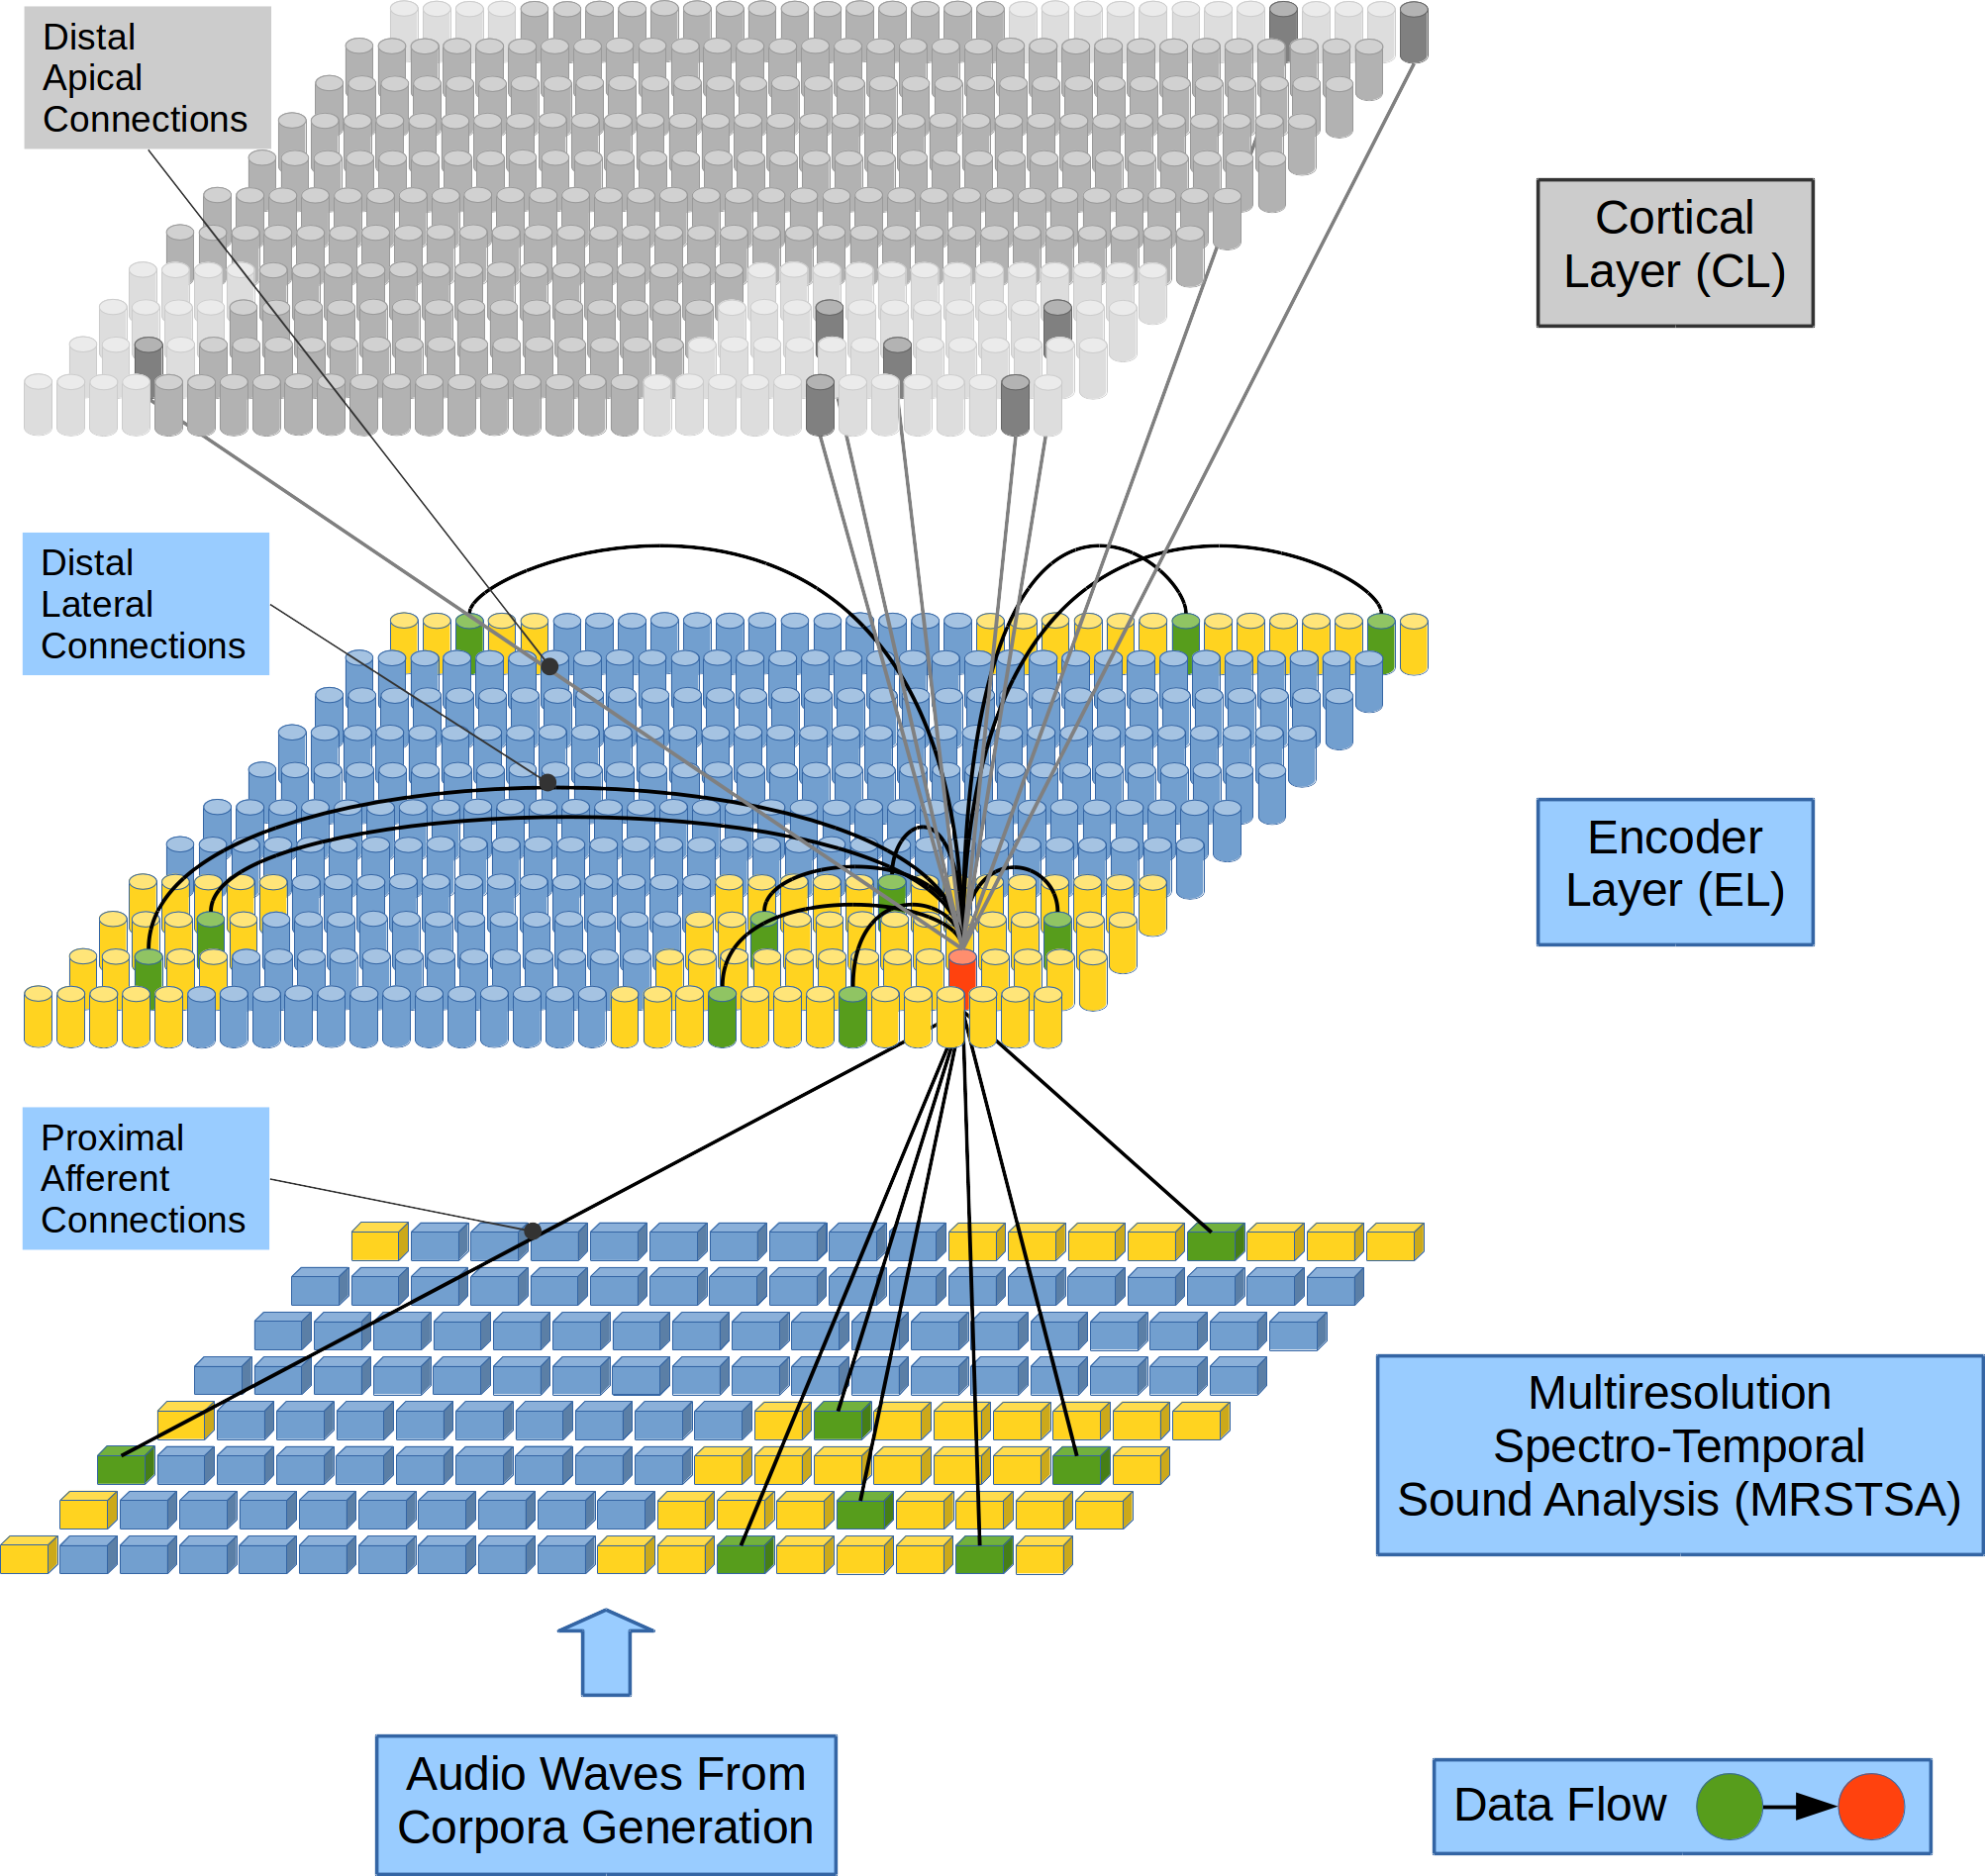
\includegraphics[width=0.5\textwidth]{EncoderColumnConnections.png}
    \caption{\gls{cstm} representation with a connection scheme for a cortical column in the Encoder Layer.
    Each cylinder in the \gls{el} and in the \gls{cl} represents a \gls{cc} in neural tissue.
    Each prism in the \gls{mrstsa} represents a real valued variable.
    This is a visualization of a \gls{cc} (in red) and its three receptive fields (in yellow).
    The receptive field of a \gls{cc} is an array that defines a set of \glspl{cc}
    with which such column could be connected.
    The receptive field of a \gls{cc} on the \gls{mrstsa} determines an array of real valued variables
    with which such column could be connected.
    A subset of \glspl{cc} in a receptive field (in green) represents the \glspl{cc} that are really
    connected with the \gls{cc} in red. A similar scenario could be described for the green prisms on
    the \gls{mrstsa}.
    The size, wrap-around property and percentage of established links (in green) inside a receptive field are tunable parameters for the model.
    In this work, only lateral connections have been implemented since in the current implementation there are no upper cortical layers from which
    to bring apical connections.}
    \label{fig:EncoderColumnConnections}
\end{figure}

The \gls{el} simulates a patch of cortical tissue using an n-dimensional array of complex structures called \glspl{csom} that simulate \glspl{cc} in the brain. The \gls{el} generates \glspl{sdr} \cite{ahmad_2016} from the inputs delivered by the \gls{mrstsa} stage and from the activation history in its own \glspl{cc}. 

Each cell unit in a \gls{cc} has two types of dendritic branches; proximal and distal. Proximal and distal dendritic branches lead to proximal and distal connections in a cell unit respectively~\cite{Dematties2018}. Neural units in the \gls{el} simulates pyramidal cells in cortical tissue in the brain (Fig \ref{fig:Pyramidal_Cell}). 

\begin{figure}[h!]
    \centering
    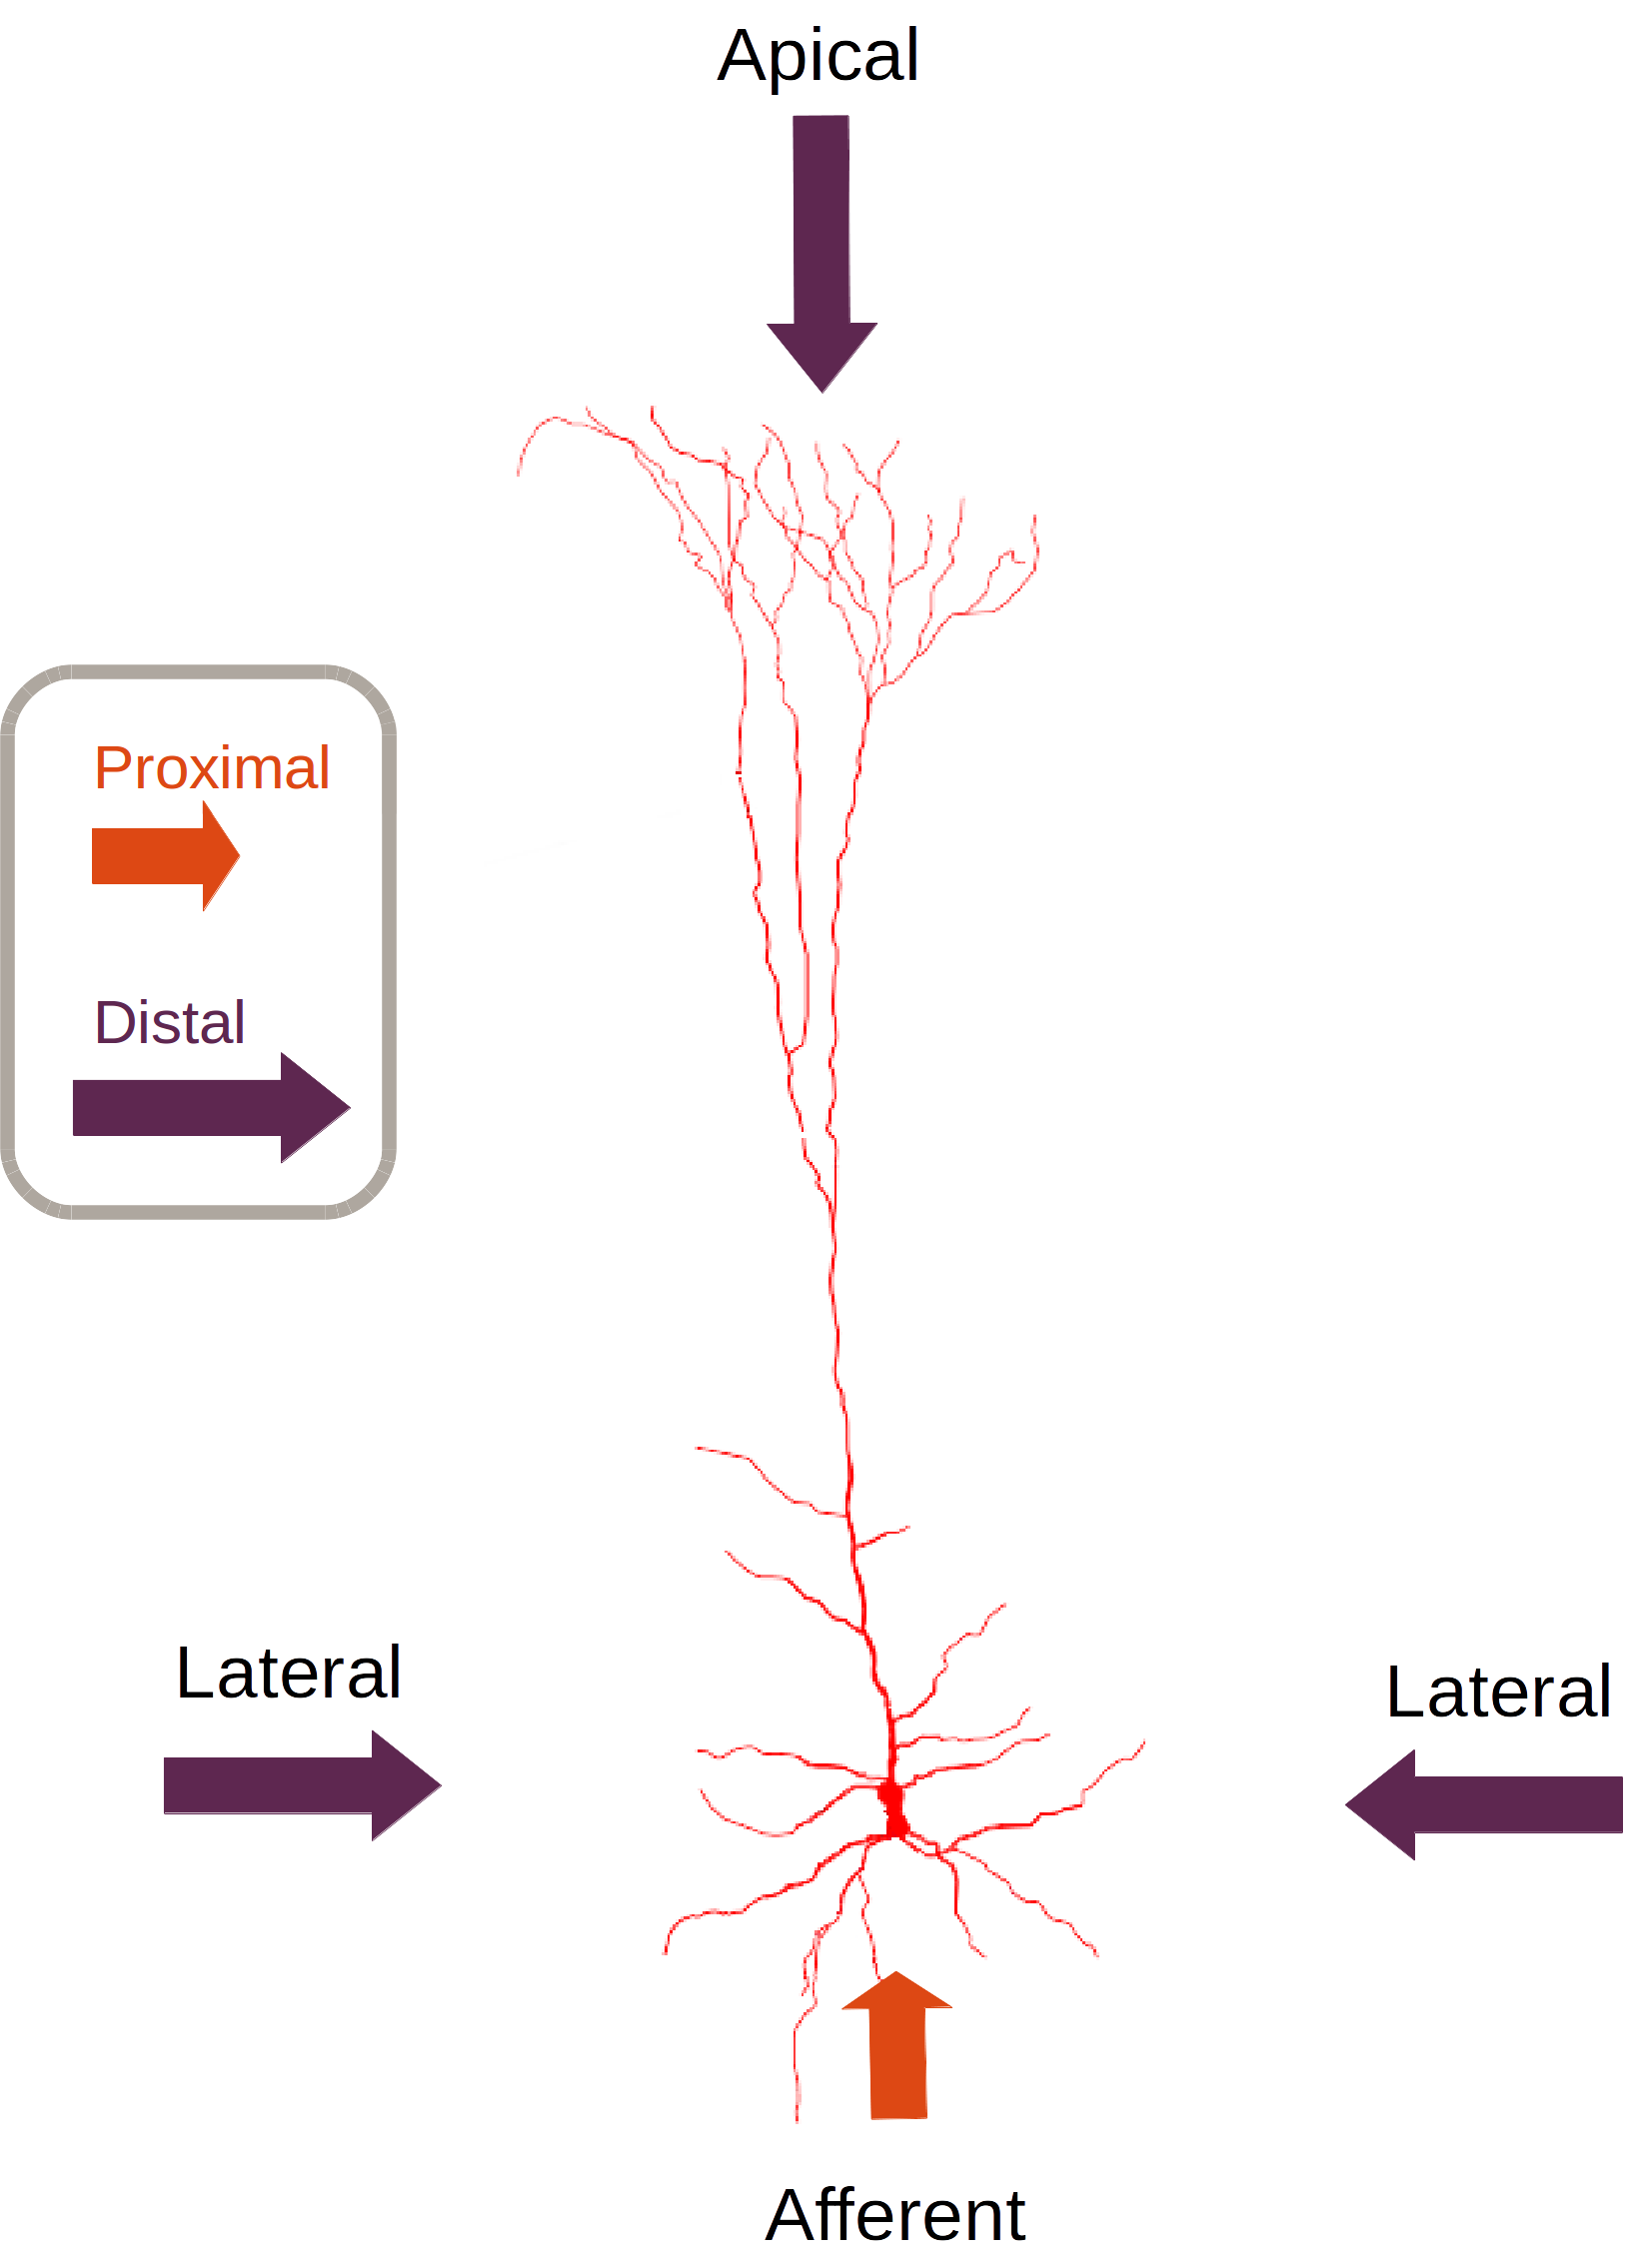
\includegraphics[width=0.3\textwidth]{Pyramidal_Cell.png}
    \caption{Connectivity profile of a pyramidal neural unit in the \gls{el}. Proximal connections are composed only by afferent connections from the \gls{mrstsa} algorithm while distal connections are composed by lateral and apical connections from neighboring columns and    from columns in another cortical layer above respectively. Adapted from (Fabuio - Own work, CC BY 4.0, \protect\url{https://commons.wikimedia.org/w/index.php?curid=60707501)}}
    \label{fig:Pyramidal_Cell}
\end{figure}













\section{Computational Implementation}

\subsection{\glsfirst{el} Implementation}







\subsubsection{\glsfirst{el} Hierarchical Inheritance and Compositional Structure}

We implemented our algorithms in the standard \CC14 using the \gls{oop} paradigm in a set of classes interrelated by inheritance and composition. We configured the~\gls{el} class as a composition of objects of class \glsfirst{csom}. The main member in the \gls{el} class is a \gls{stl} vector of \gls{csom} objects. Each \gls{csom} object in the \gls{stl} vector represents a \gls{cc} in the \gls{el}. A complete diagram of the hierarchical inheritance and compositional structure of the implementation can be seen in Fig. \ref{fig:InheritanceComposition}.

\begin{figure}[h!]
    \centering
    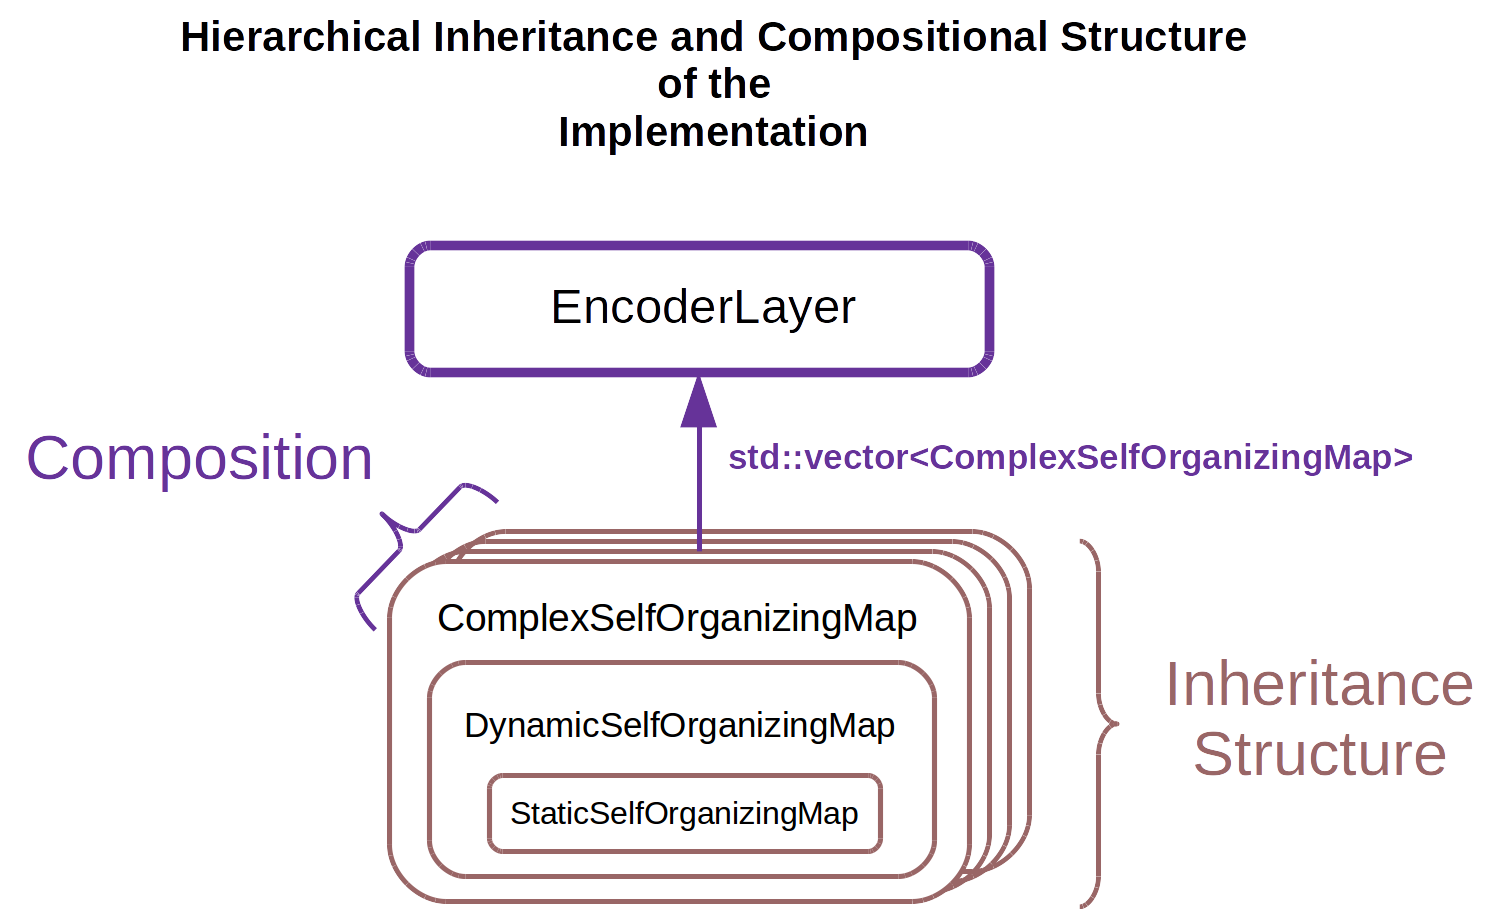
\includegraphics[width=0.5\textwidth]{InheritanceComposition.png}
    \caption{Hierarchical Inheritance and Compositional Structure of the \gls{el}. \glsfirst{csom} inherits from \glsfirst{dsom} which inherits from \glsfirst{ssom}. The \glsfirst{el} is composed by a set of \glspl{csom} gathered    in a std::vector \glsfirst{stl} container.}
    \label{fig:InheritanceComposition}
\end{figure}

The \glsfirst{ssom} class implements proximal connections, the \glsfirst{dsom} class implements distal connections and the \glsfirst{csom} class implements activation rules in a~\gls{cc} \cite{Dematties2018}. Each class uses \gls{stl} vectors to store its data and \texttt{<algorithm>} \gls{stl} library to computationally operate through iterators or pointers on those vectors.










\subsubsection{\glsfirst{el} Parallelization}
\label{EL_Parallelization}

We parallelized the \gls{el} class by means of a hybrid \gls{mpi}+\gls{omp} paradigm distributing \glspl{csom} among \gls{mpi} ranks as a deck of cards is distributed among different players. Each \gls{mpi} rank ends up with one or more \glspl{csom} and the \glspl{csom} in each rank are distributed among different \gls{omp} threads (Fig. \ref{fig:Encoder_Parallelization}).% and Alg.~\ref{ccs_distribution}).

%\begin{algorithm}
	%\caption{This algorithm distributes \glspl{cc} among \gls{mpi} processes in a distributed memory system and the \glspl{cc} in each process are distributed among \gls{omp} threads in a shared memory system. In this algorithm we run one \gls{mpi} process per compute node on Cooley.}
%\label{ccs_distribution}
%\begin{algorithmic}[1]
	%\STATE {\texttt{numberOfProcesses} = getNumberOfProcesses()}
	%\STATE {\texttt{processNumber} = getProcessNumber()}
	%\STATE {\#\textbf{pragma omp parallel for} default(none) shared(\texttt{processNumber}, \texttt{numberOfProcesses})}
	%\FOR{\texttt{column} = \texttt{processNumber} \TO \texttt{column} = number of \glspl{cc}; \texttt{column} += \texttt{numberOfProcesses}}
	%\STATE {Do \gls{csom} stuff...}
	%\ENDFOR
%\end{algorithmic}
%\end{algorithm}

\begin{figure}[h!]
    \centering
    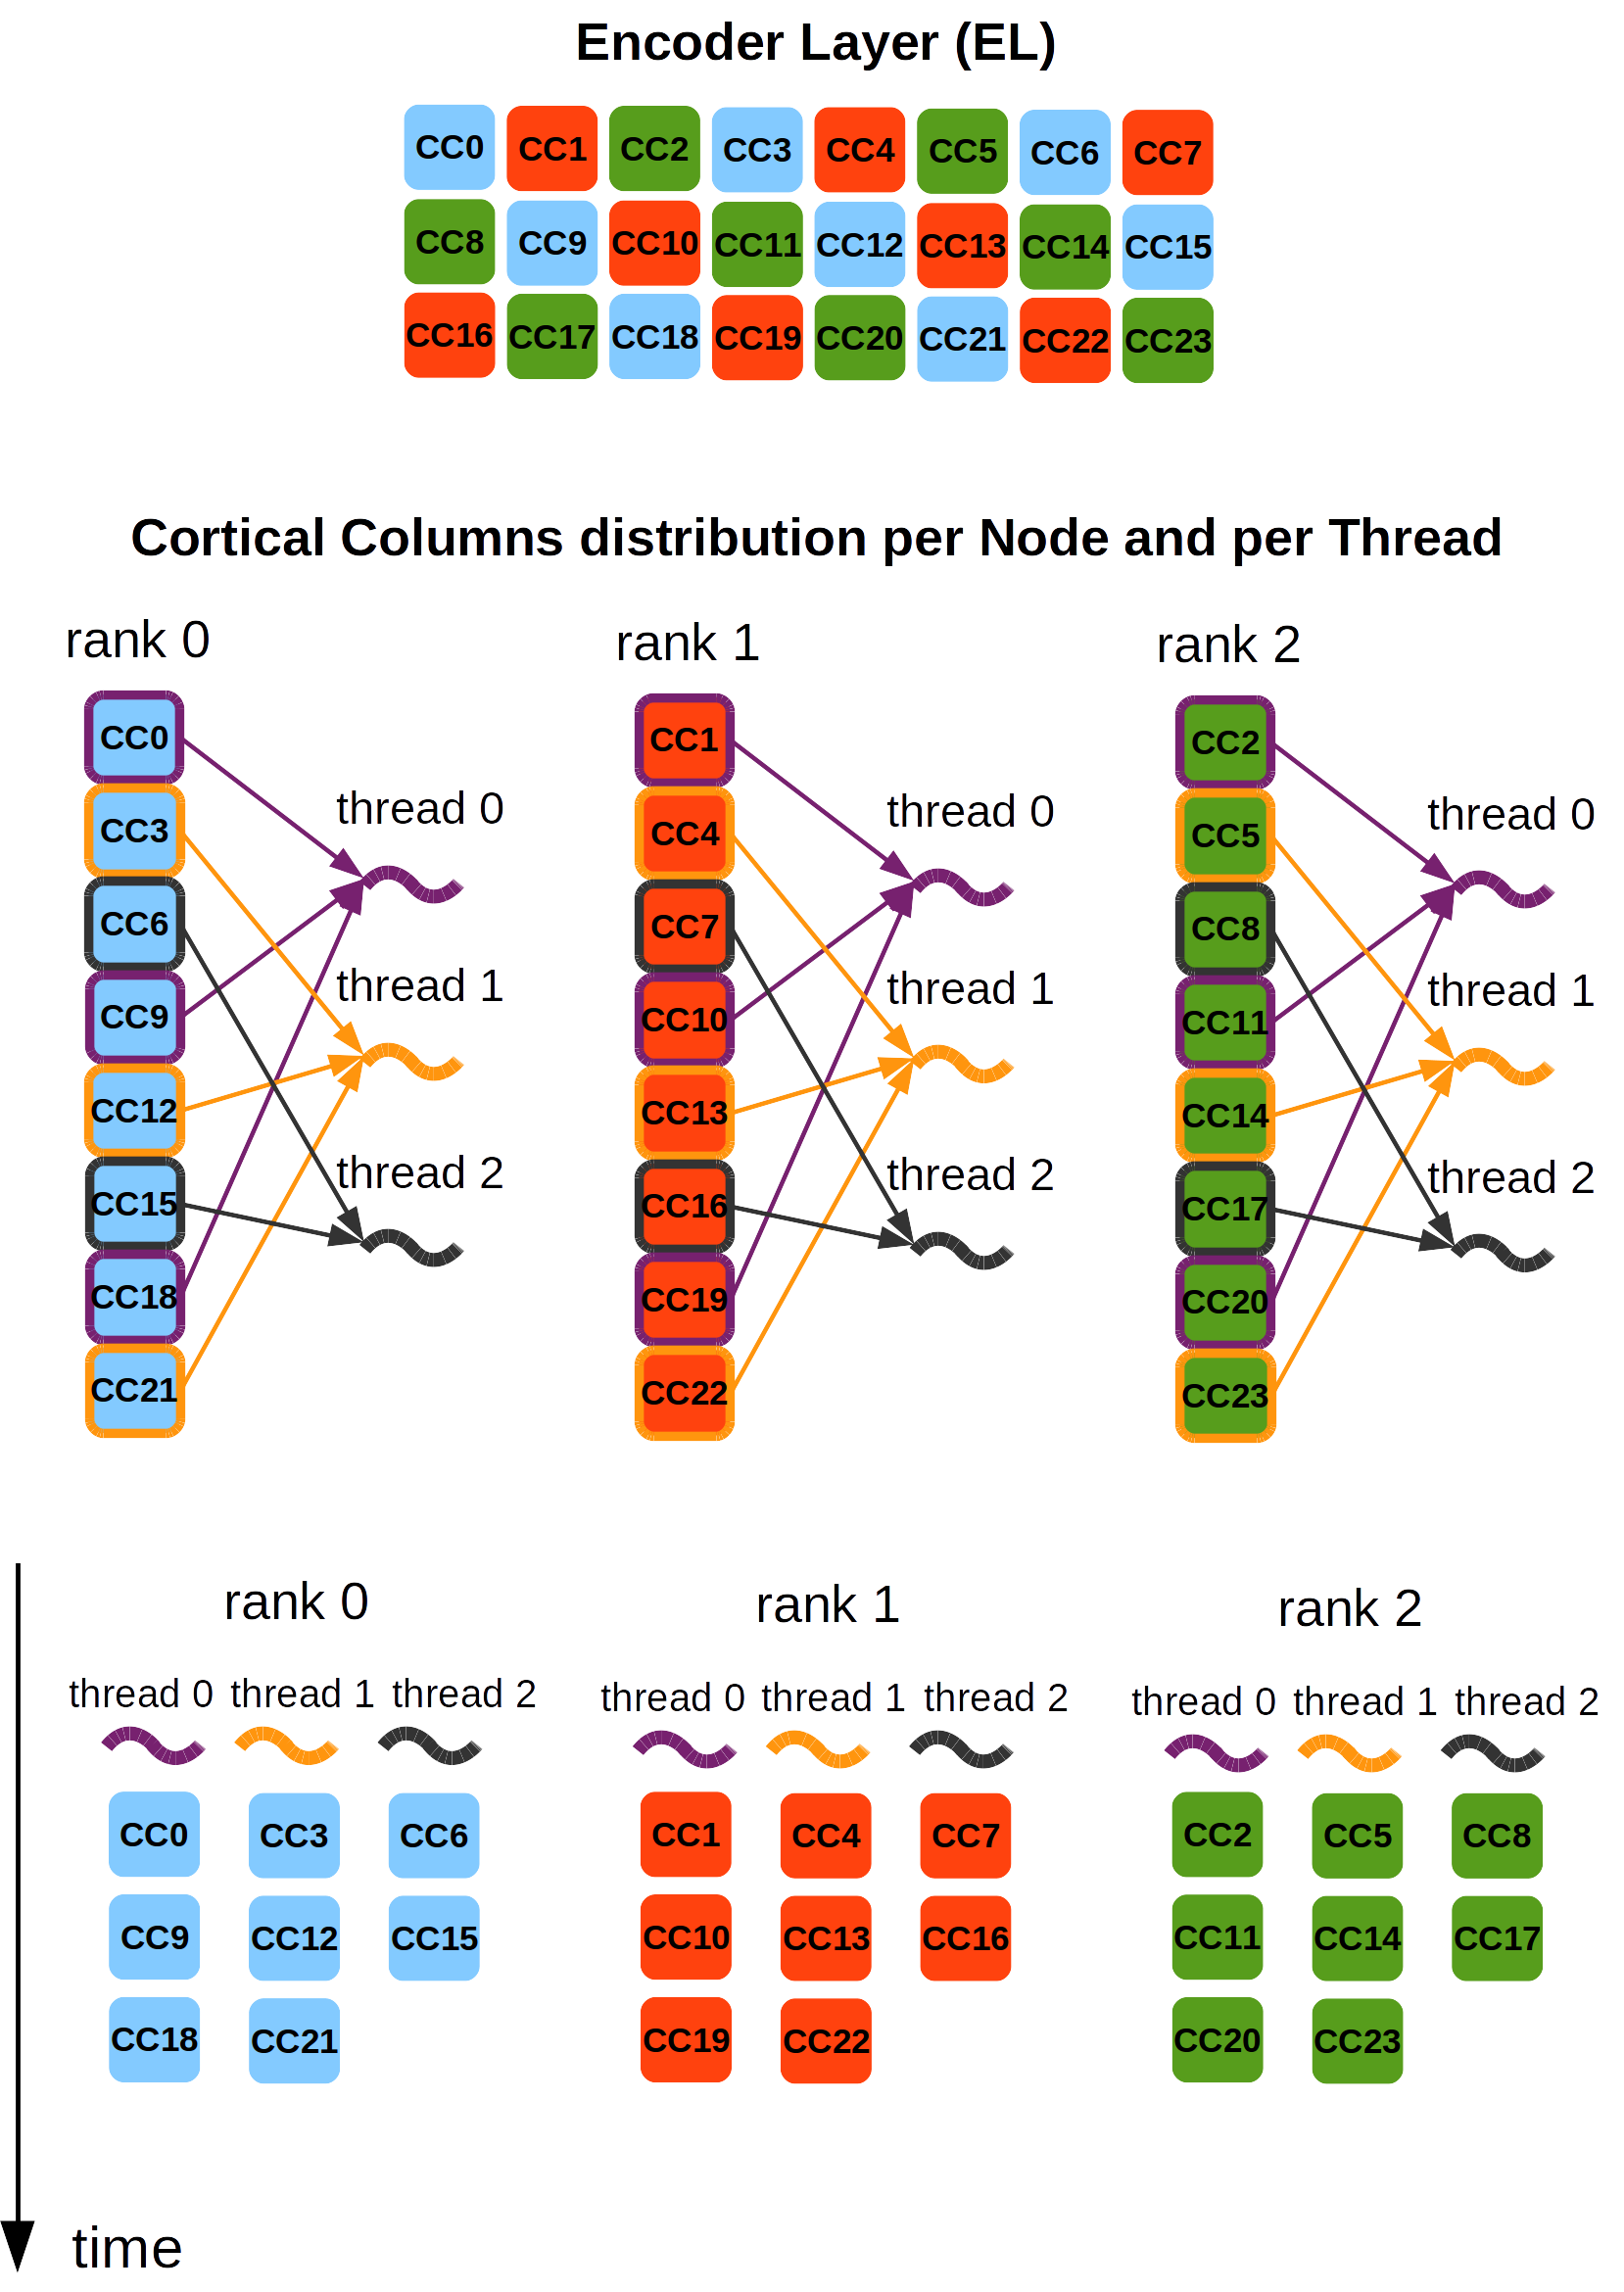
\includegraphics[width=0.45\textwidth]{Encoder_Parallelization.png}
    \caption{\glsfirst{el} \gls{mpi}+\gls{omp} parallelization. Distribution of \gls{csom} objects in an \gls{el} with 3 by 8 (24) \glspl{cc} among three \gls{mpi} ranks with three \gls{omp} threads per rank. Certain ranks could take care of a different number of \glspl{csom} depending on the number of \gls{mpi} ranks as well as the number of \glspl{cc} in the \gls{el}. Each \gls{mpi} rank distributes its \glspl{csom} among different threads in the same fashion.}
    \label{fig:Encoder_Parallelization}
\end{figure}

Information among \gls{mpi} ranks must be transferred in each time step. Basically all the information needed by each process is the identity of the active neural units in each \gls{cc} of the \gls{el}. We gather all the information corresponding to the \glspl{csom} in each rank and then use \gls{mpi} Bcast function to transmit such information using a special comunication protocol by means of which we specify the boundaries in the information corresponding to each \gls{csom}(Fig. \ref{fig:BCast}). By means of this strategy each \gls{mpi} rank has to call \gls{mpi} Bcast just once in order to transmit its data.

\begin{figure}[h!]
    \centering
    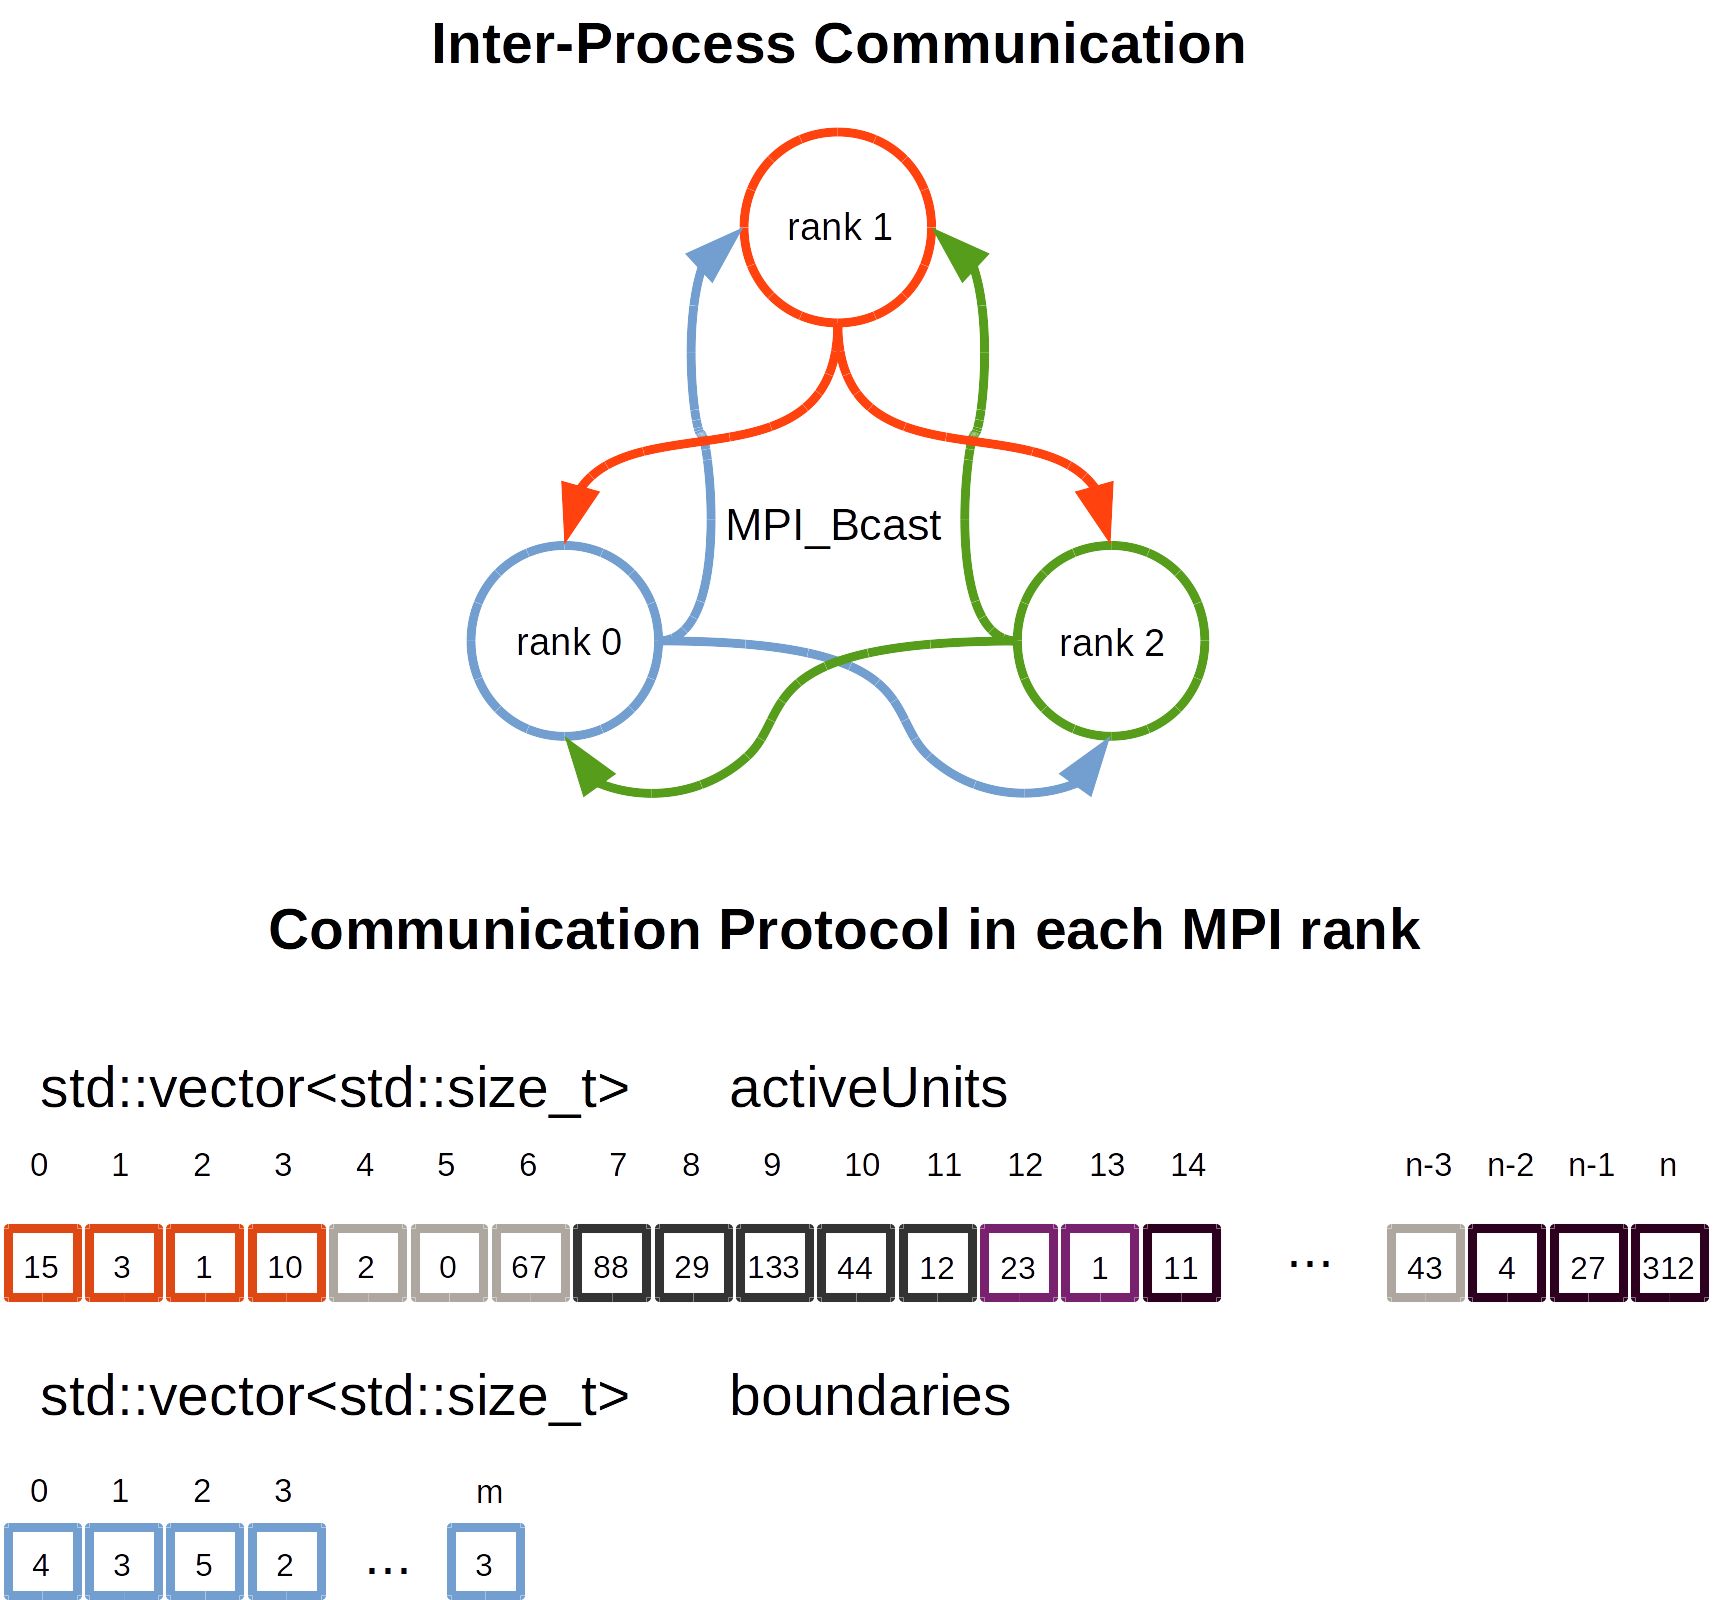
\includegraphics[width=0.45\textwidth]{BCast.png}
    \caption{ \gls{mpi} \gls{ipc} among different ranks. \gls{ipc} is carried out at each time step since each \gls{mpi} rank requires the complete \gls{el} output at each time step. Each \gls{mpi} rank broadcasts the information corresponding to its \glspl{cc} to the other ranks in the \gls{mpi} environment. In the communication protocol to transmit information among \gls{mpi} ranks in the \gls{el} all the information is transmitted in two \gls{stl} vectors--\texttt{activeUnits} and \texttt{boundaries}. The vector \texttt{activeUnits} identifies the active neural units in the \glspl{cc} inside a \gls{mpi} rank and \texttt{boundaries} identifies the number of active units that belong to different \glspl{cc}. There are $n+1$ active units in the \glspl{cc} managed by certain \gls{mpi} rank and there are $m+1$ \glspl{cc} managed by such \gls{mpi} rank.}
    \label{fig:BCast}
\end{figure}

The \gls{el} uses \gls{mpi} I/O parallel file system to save its status in Matlab/Octave format (Fig. \ref{fig:MPI_IO}). Each \gls{mpi} rank gathers all the data corresponding to its \glspl{csom} in the \gls{el} and puts such data--formated in Matlab/Octave--in a \texttt{std::stringstream} class. Then such \gls{mpi} rank communicates the part of the file it will use to the other \gls{mpi} ranks in order to store the data without interfering with the other ranks in the \gls{mpi} environment. Finally, each \gls{mpi} rank saves all its data with a unique call to \gls{mpi} Write using the complete \texttt{std::stringstream}.

\begin{figure}[h!]
    \centering
    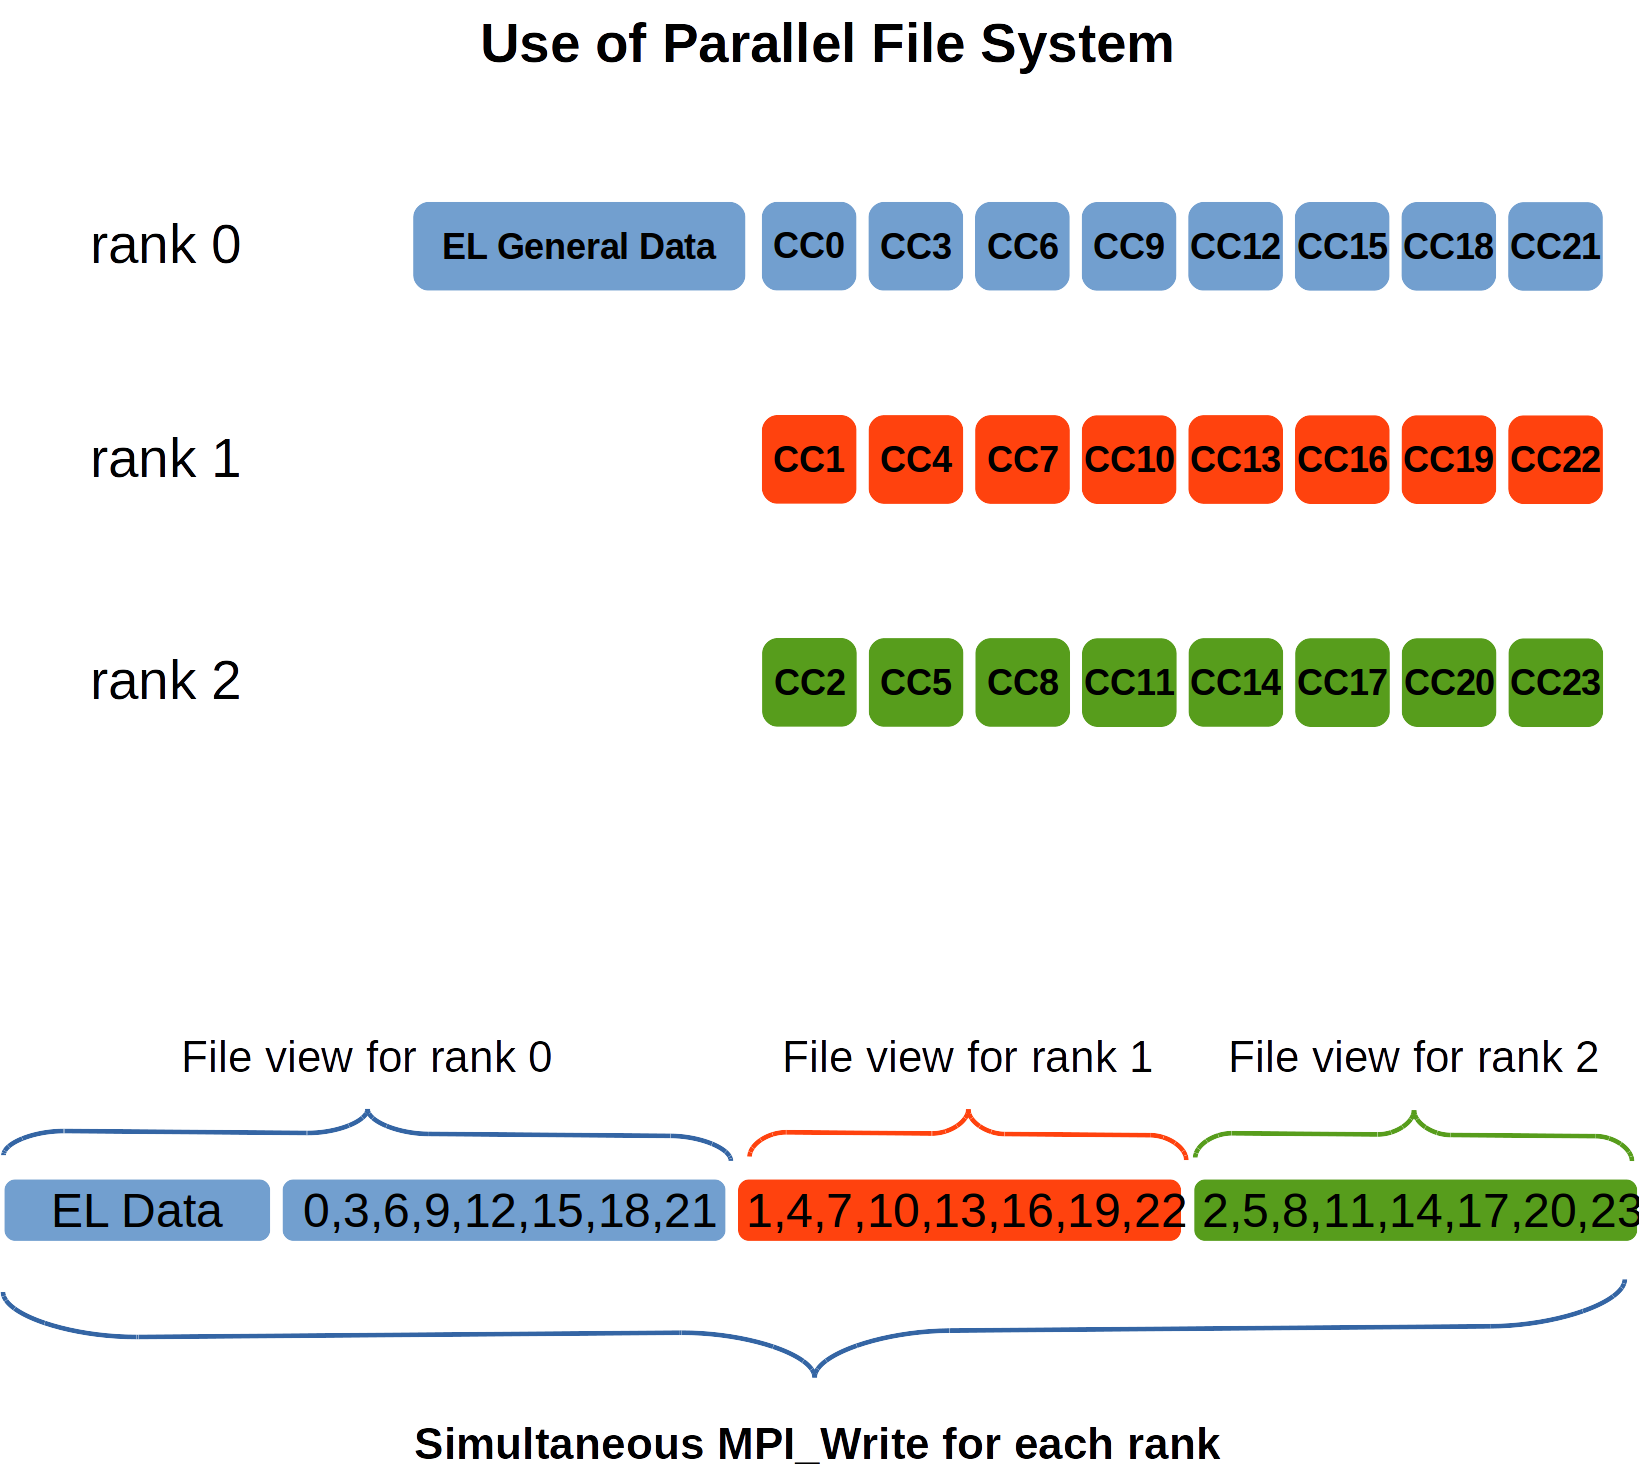
\includegraphics[width=0.5\textwidth]{MPI_IO.png}
    \caption{\gls{el} information distribution in a file to save its status. Each \gls{mpi} rank puts the formated data corresponding to its \glspl{csom} in a \gls{stl} \texttt{stringstream} class template. Rank 0 also takes care of the \gls{el} structure, connectivity and parameters. Once each rank has its \texttt{stringstream} with the formated data, it communicates its file view to the other ranks. Then each rank writes its stream of bytes in parallel without interfering with other ranks in the \gls{mpi} environment. An \gls{el} with a different number of ranks can load the same file without affecting the final results. Each rank in the new \gls{el} loads the complete file in a \gls{stl} \texttt{stringstream} class template and then takes the informations that concern it from such structure.}
    \label{fig:MPI_IO}
\end{figure}

In this work, each \gls{mpi} rank runs in a diferent Cooley node and keeps all the data that corresponds to the \gls{el} object, such as \gls{el} dimensionality, receptive fields for each \gls{cc}, percentages of real connections in each receptive field for each \gls{cc}, population dimensionalities for the \glspl{cc} as well as the complete connectivity of each \gls{cc} and all the general parameters of the model such as learning rates, learning neighborhoods, etc~\cite{Dematties2018}. Although this general \gls{el} data is replicated in each \gls{mpi} rank this is not significant compared to the data corresponding to the \glspl{csom} objects. Each \gls{mpi} rank keeps only the data for those \glspl{csom} which are under its charge. Fig. \ref{fig:EL_ALG} depicts the general layout that follows the \gls{el} algorithm.

\begin{figure*}[ht]
    \centering
    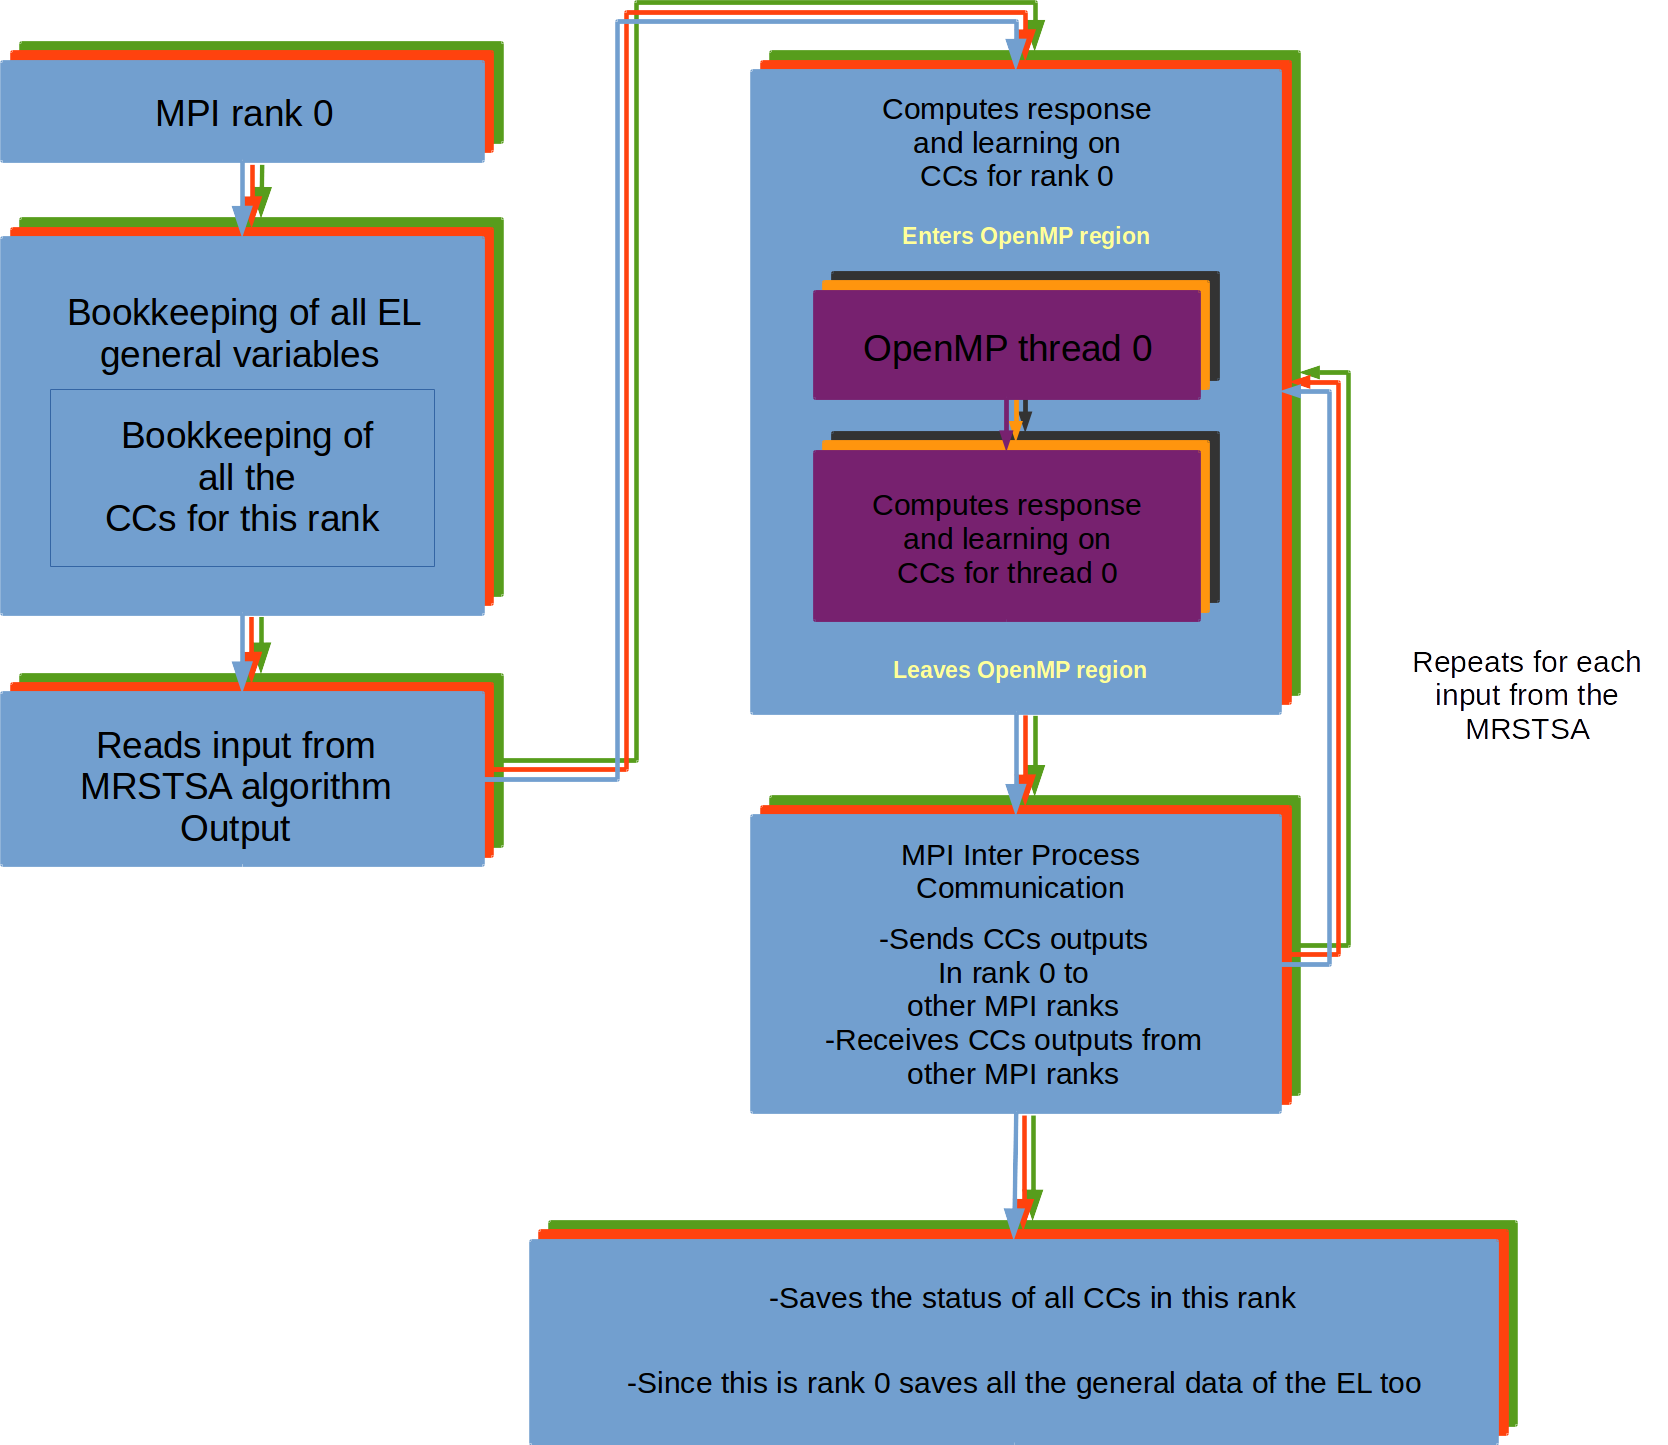
\includegraphics[width=0.7\textwidth]{EL_ALG.png}
    \caption{General layout of the \gls{el} algorithm. Each \gls{mpi} rank keeps a private copy of the entire \gls{el} structure but only keeps the data of the \glspl{csom} which correspond to it. Each \gls{mpi} rank loads a private copy of the inputs that come from the \gls{mrstsa} algorithm. Then each \gls{mpi} rank processes the input information by means of only the \glspl{cc} which are under its charge, first entering to an \gls{omp} region in order to distribute \glspl{cc} in the rank among different \gls{omp} threads and then leaving the \gls{omp} region and communicating the outputs of all \glspl{cc} in the \gls{el} using \gls{mpi} \gls{ipc} tools. Finally each \gls{mpi} rank saves the status of its \glspl{cc} using \gls{mpi} parallel I/O sentences. \gls{mpi} rank 0 also saves the general structure of the \gls{el}.} 
    \label{fig:EL_ALG}
\end{figure*}














\subsection{\gls{mrstsa} Implementation}

We implemented the \gls{mrstsa} algorithm in C using the package FFTW~\cite{fftw} which is an implementation of the \gls{fft} available on Cooley. We used \gls{mpi}+\gls{omp} hybrid parallelization approach. We parallelized the \gls{mrstsa} algorithm developed in \cite{Dematties2018} by means of \gls{omp} sections using one \gls{omp} section per spectral resolution and running until 5 \gls{omp} threads per Cooley node (Fig.~\ref{sub:MRSTSA_Parallelization}). In terms of \gls{mpi} we processed a set of corpora per \gls{mpi} rank. The algorithm generates certain number of corpora per vocabulary. Supposing that we have $n$ vocabularies and $m$ corpora per vocabulary, we end up with $n m$ corpora. Unlike the corpora generation parallelization algorithm exposed in Alg.~\ref{fig:CorporaGenerationParallelization} and explained in section~\ref{CorpGenImp} in this case we unroll the nested loop that iterates through corpora and vocabularies. The \gls{mpi} parallelization is exposed in Fig.~\ref{sub:MRSTSA_ALG}.

%\begin{algorithm}
	%\caption{This algorithm is called \gls{mrstsa} and distributes the different spectral resolutions--processing a corpus--among \gls{omp} threads running until 5 \gls{omp} threads concurrently in order to generate such corpus processing.}
%\label{MRSTSA_parallelization}
%\begin{algorithmic}[1]
	%\STATE {\#\bf{pragma omp parallel sections}}
	%\STATE {~~\#\bf{pragma omp section}}
	%\STATE {~~~~Do stuff...}
	%\STATE {~~\#\bf{pragma omp section}}
	%\STATE {~~~~Do stuff...}
	%\STATE {~~\#\bf{pragma omp section}}
	%\STATE {~~~~Do stuff...}
	%\STATE {~~\#\bf{pragma omp section}}
	%\STATE {~~~~Do stuff...}
	%\STATE {~~\#\bf{pragma omp section}}
	%\STATE {~~~~Do stuff...}
%\end{algorithmic}
%\end{algorithm}

%\begin{algorithm}
	%\caption{This algorithm distributes corpora among \gls{mpi} processes and each \gls{mpi} process run until 5 \gls{omp} threads concurrently in order to generate each corpus. In this algorithm we run one \gls{mpi} process per Cooley node.}
%\label{input_generation_parallelization}
%\begin{algorithmic}[1]
	%\STATE {\texttt{numberOfProcesses} = getNumberOfProcesses()}
	%\STATE {\texttt{processNumber} = getProcessNumber()}
	%\FOR{\texttt{task} = 0 \TO \texttt{task} = \texttt{numberOfVocabularies} * \texttt{numberOfCorpora}}
		%\STATE {\texttt{corpus} = (\texttt{int})\texttt{task}/\texttt{numberOfVocabularies}}
		%\STATE {\texttt{vocabulary} = \texttt{task}\%\texttt{numberOfVocabularies}}
		%\STATE {MRSTSA(\texttt{corpus}, \texttt{vocabulary})}
	%\ENDFOR
%\end{algorithmic}
%\end{algorithm}

The complete parallelization scheme is depicted in Fig.~\ref{fig:MRSTSA_Parallelization}. Corpora are distributed among \gls{mpi} ranks as a deck of cards is distributed among players. Each \gls{mpi} rank ends up with a set of corpora which it processes one at a time--sequentially. Each corpus processing runs 5 \gls{omp} threads concurrently in order to process the spectral resolutions of the corpus. 

\begin{figure*}[tb] 
    \centering
  \subfloat[This algorithm distributes corpora among \gls{mpi} processes and each \gls{mpi} process run until 5 \gls{omp} threads concurrently in order to generate each corpus.\label{sub:MRSTSA_ALG}]{%
       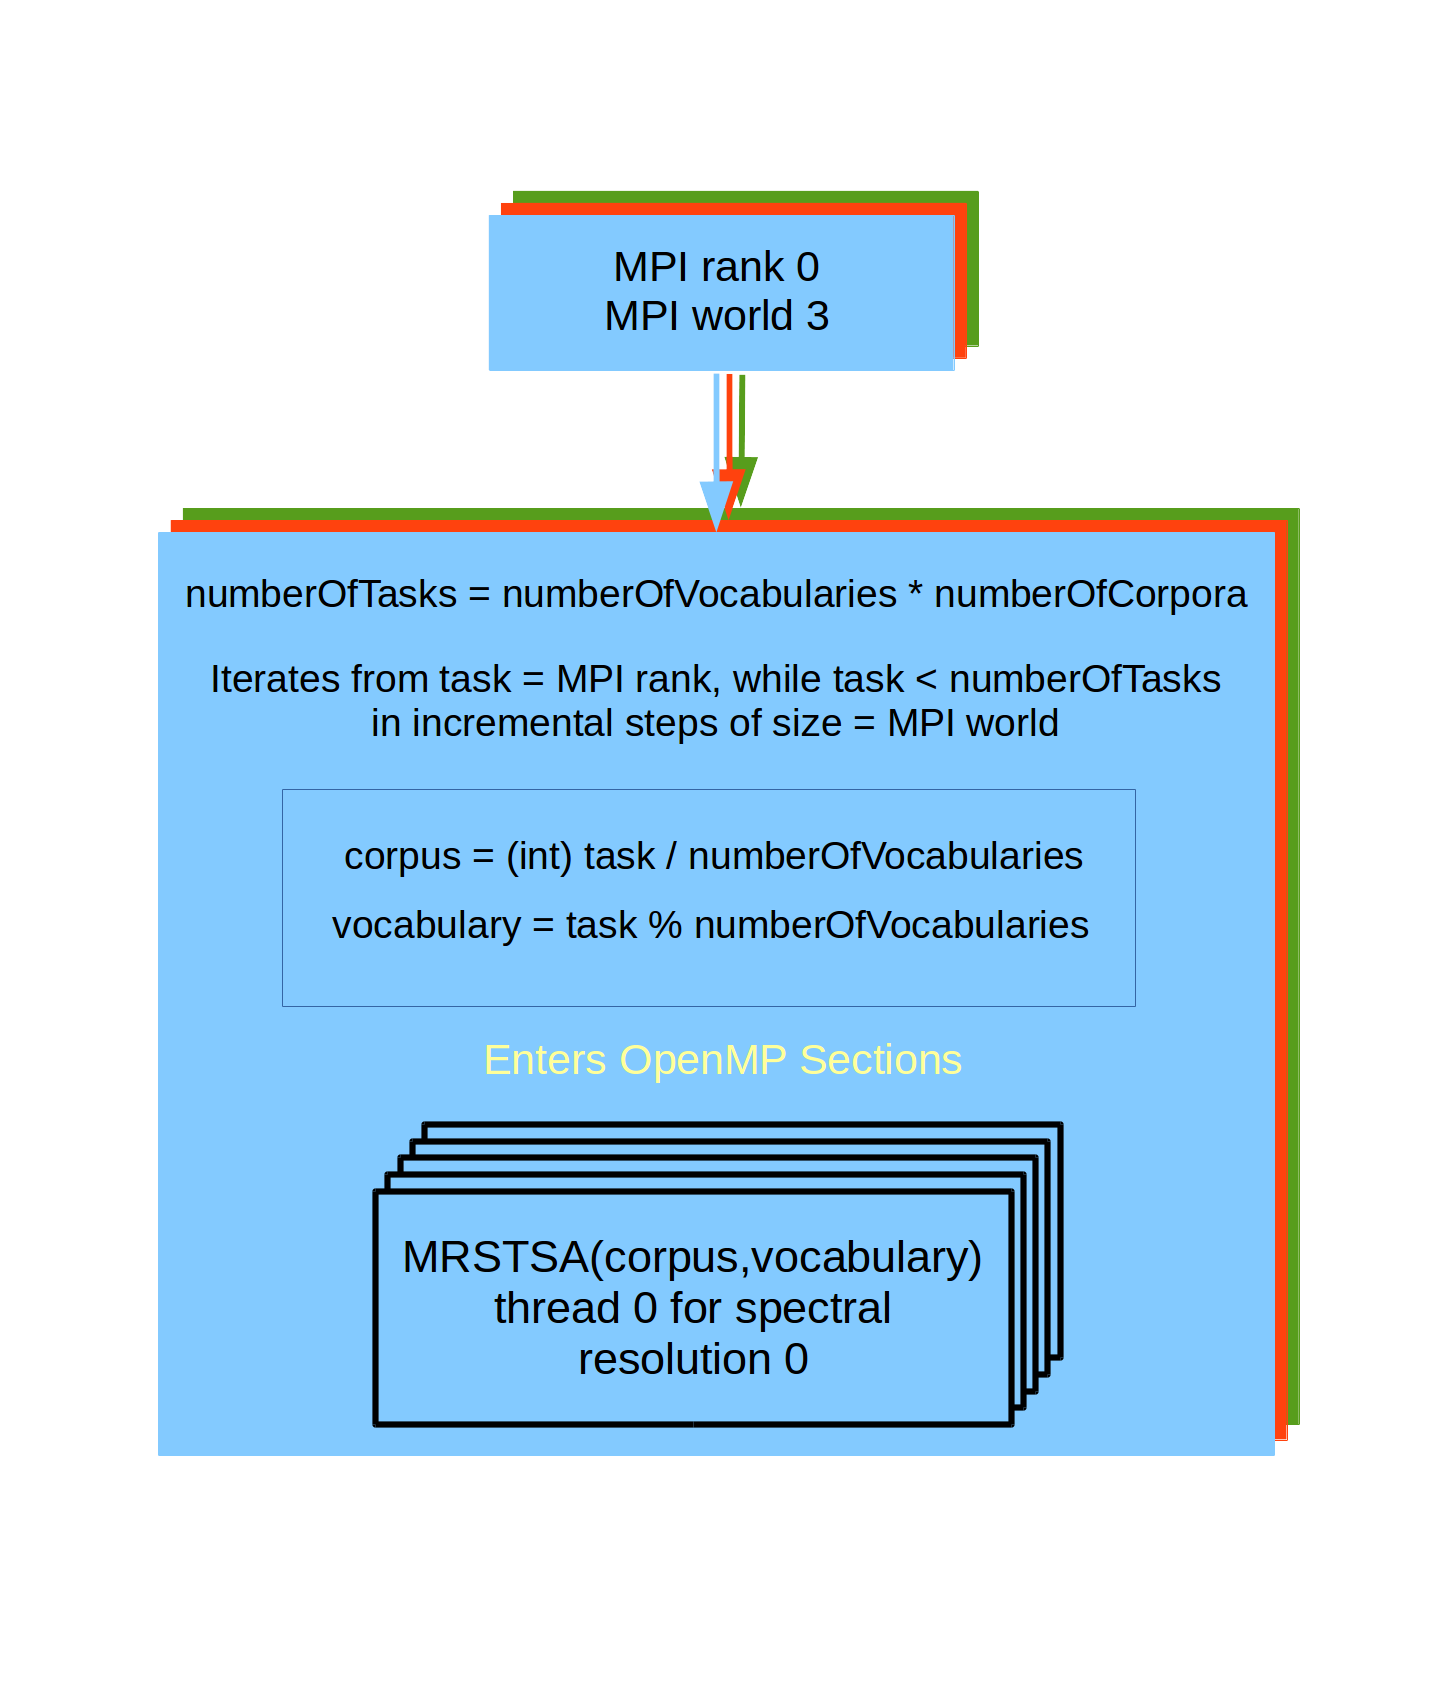
\includegraphics[width=0.49\linewidth]{MRSTSA_ALG.png}}
    \hfill
  \subfloat[Ten corpora processing are distributed among \gls{mpi} ranks. Each rank processes one corpus at a time sequentially but each corpus spectral resolution is processed concurrently by means of \gls{omp} threads.\label{sub:MRSTSA_Parallelization}]{%
        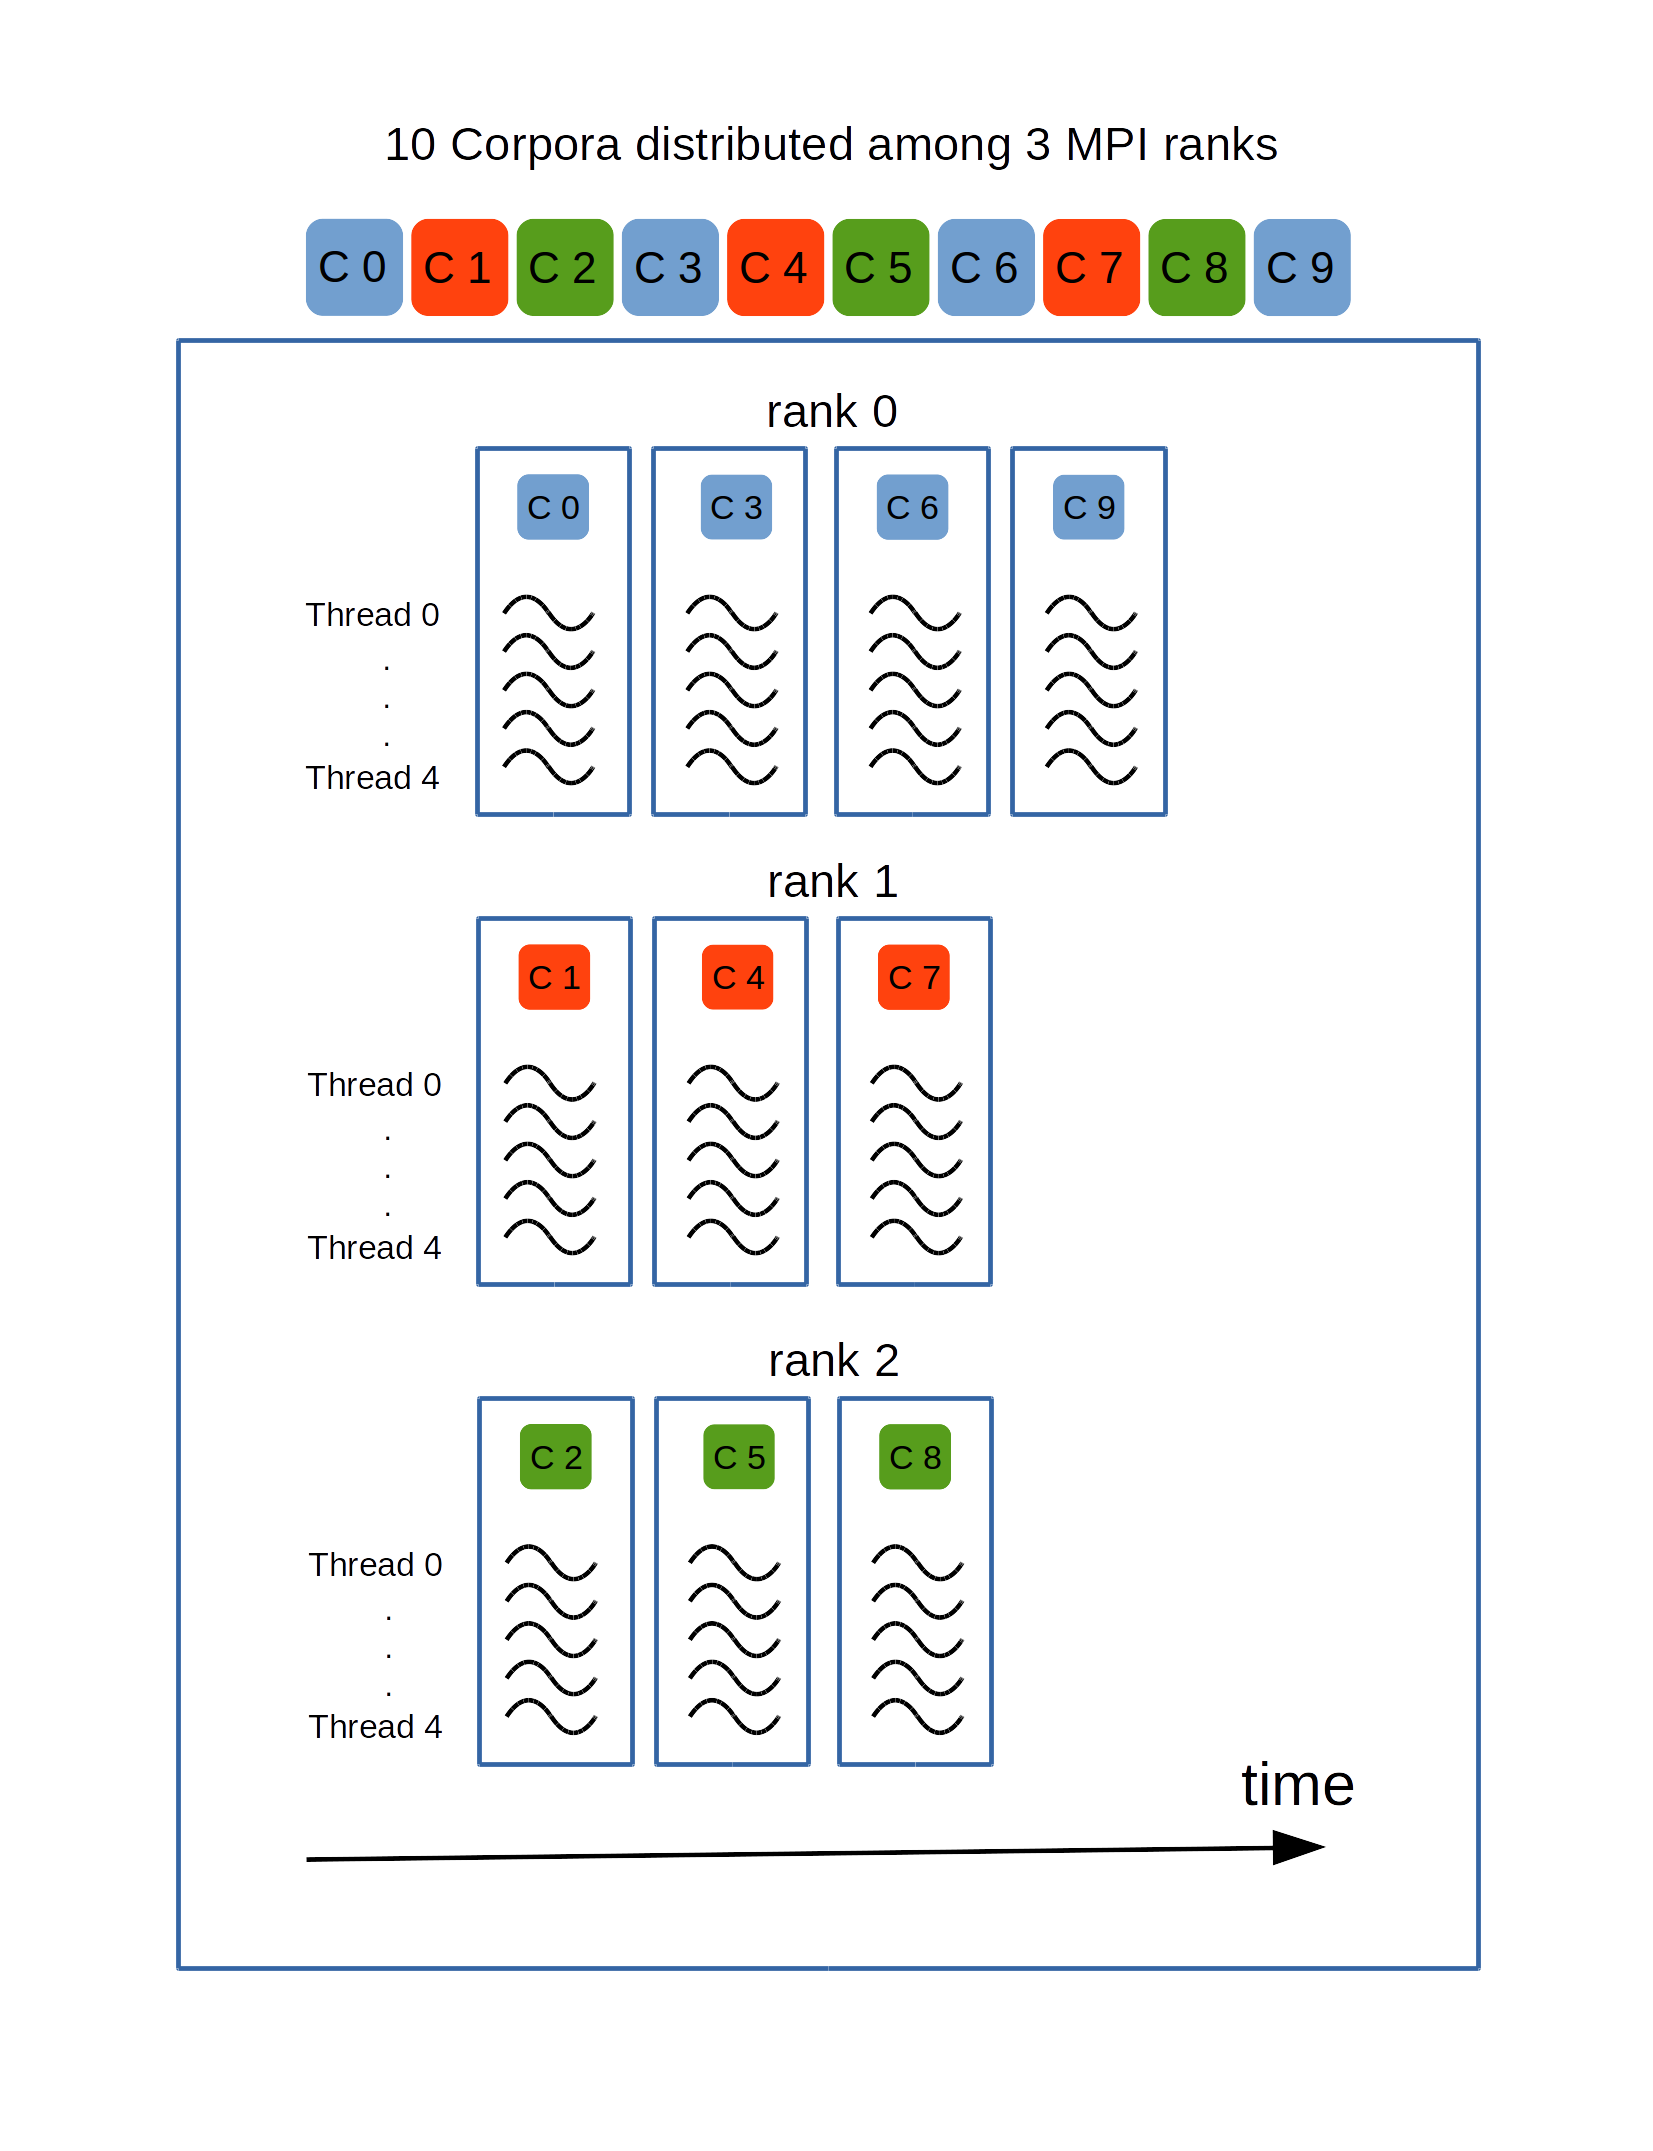
\includegraphics[width=0.49\linewidth]{MRSTSA_Parallelization.png}}
	\caption{Parallelization scheme for the \gls{mrstsa}. In this algorithm we run one \gls{mpi} process per Cooley node. The \gls{mrstsa} algorithm distributes the different spectral resolutions--processing a corpus--among \gls{omp} threads running until 5 \gls{omp} threads concurrently in order to generate such corpus processing.}
  \label{fig:MRSTSA_Parallelization} 
\end{figure*}

%\begin{figure}[h!]
    %\centering
    %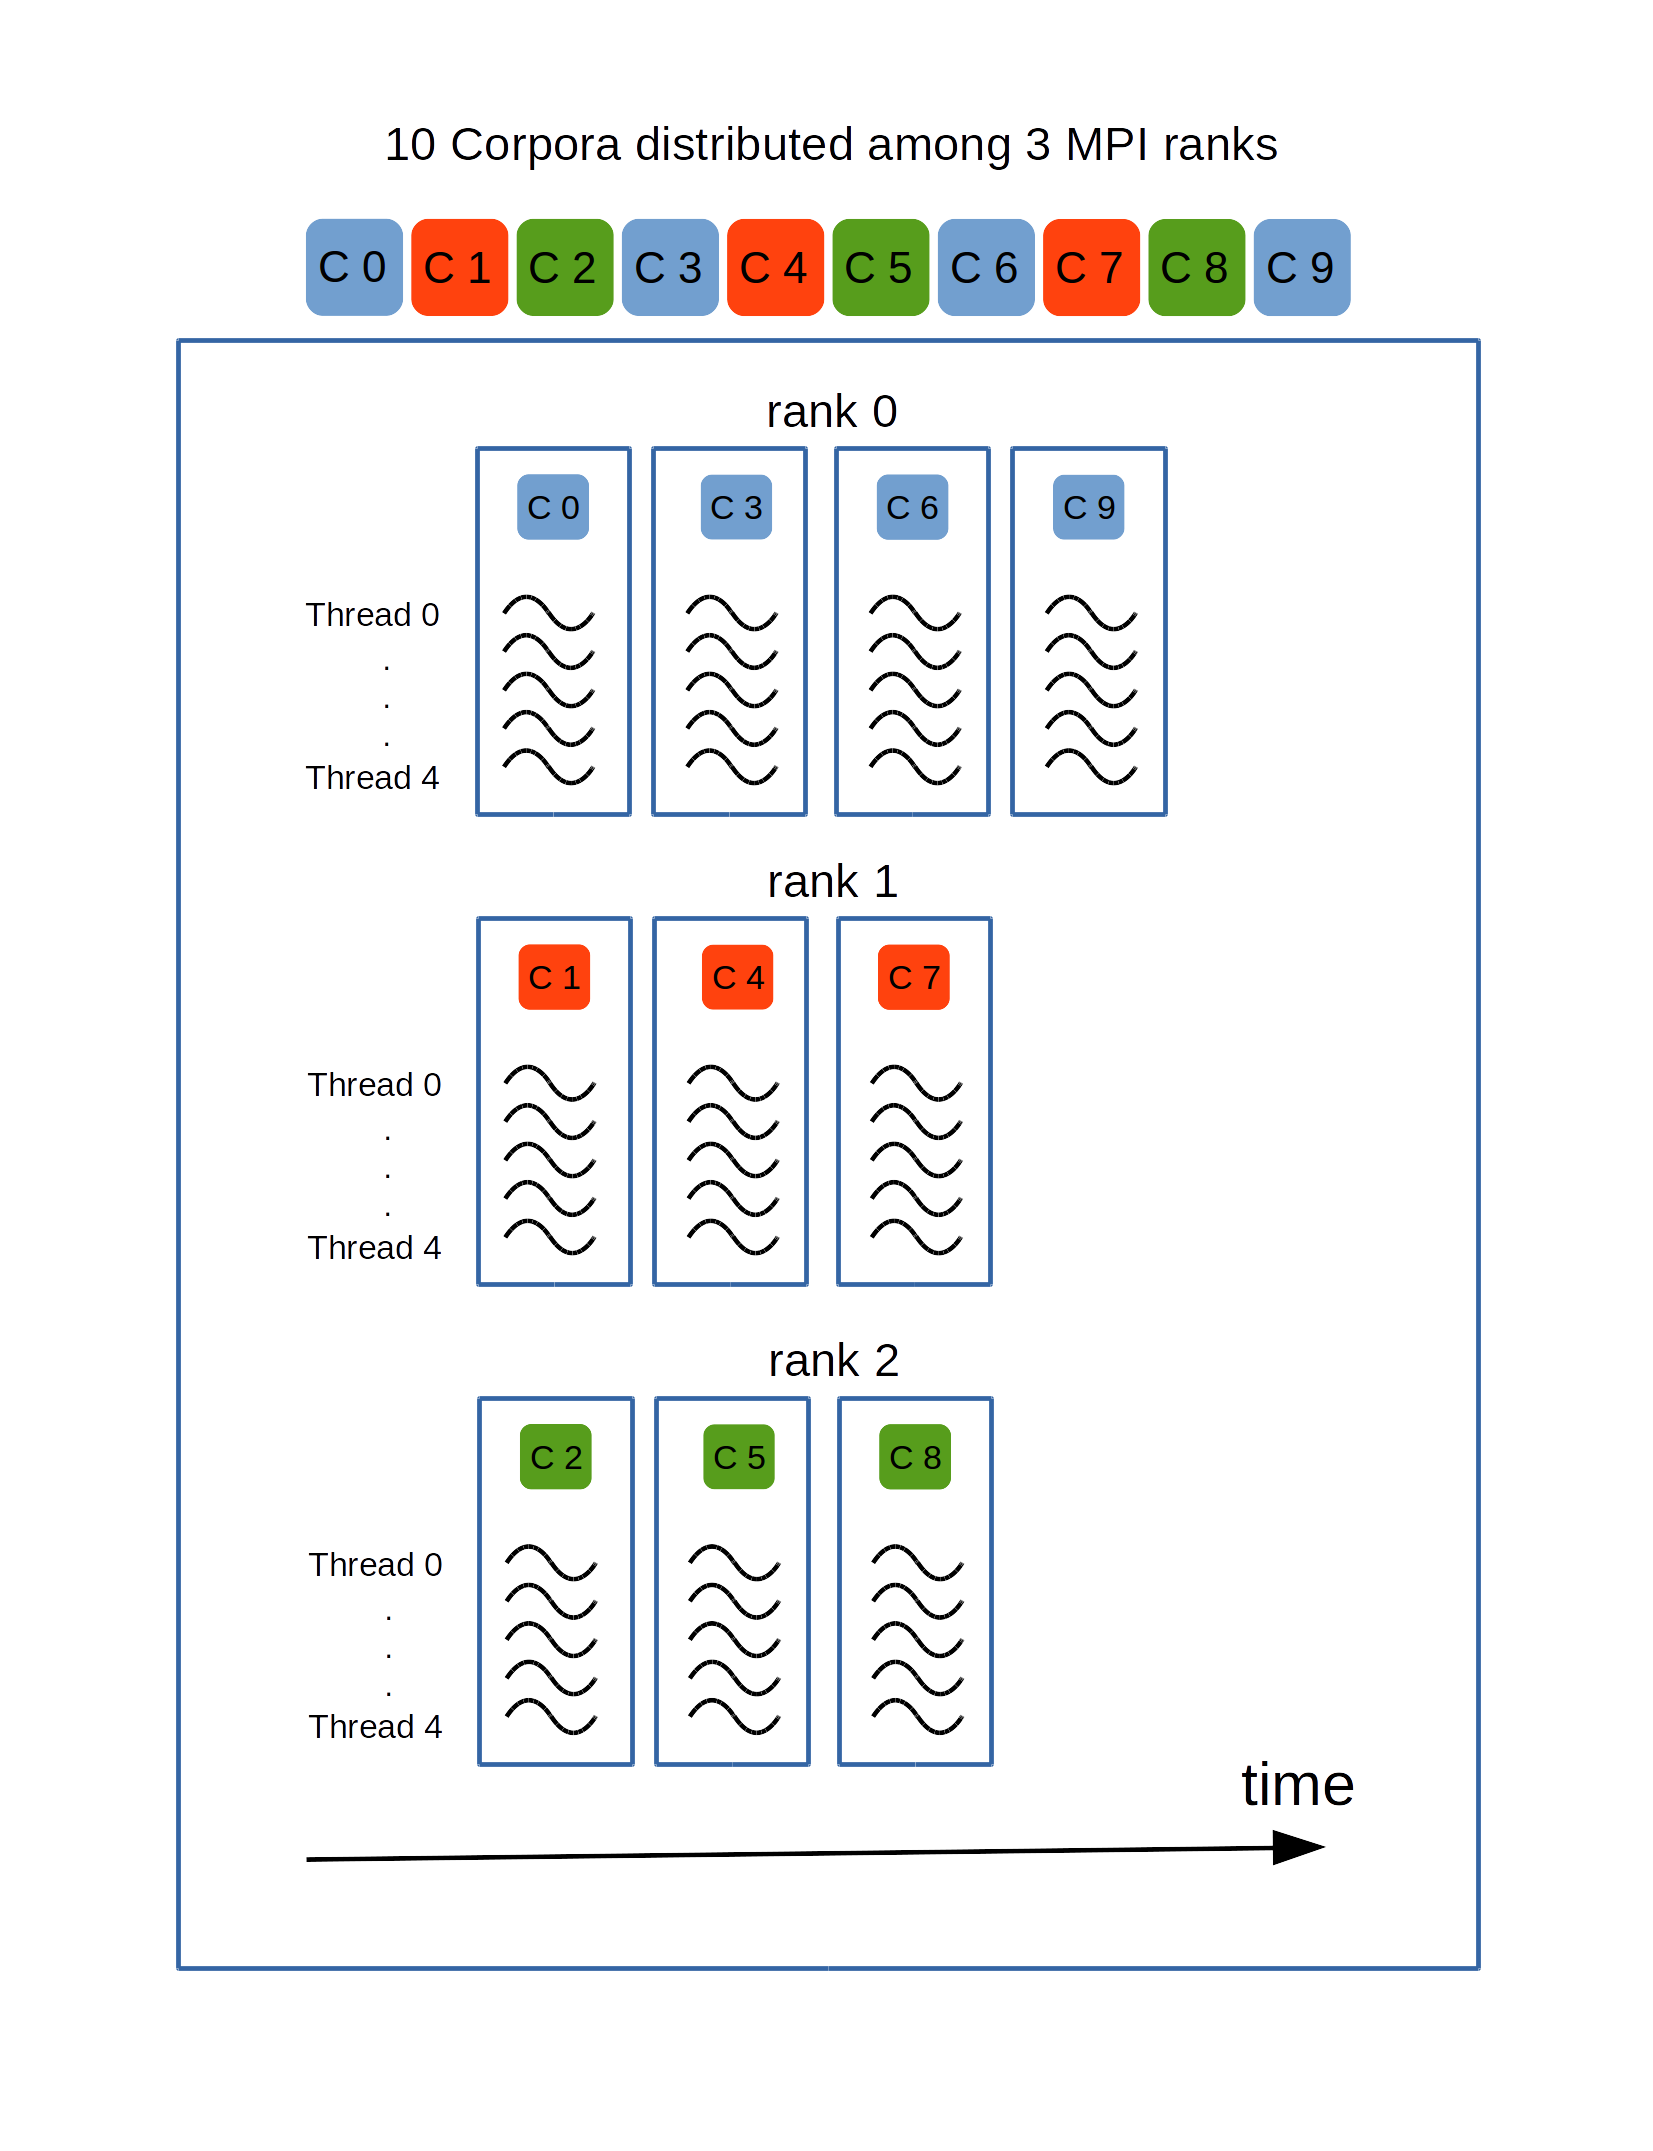
\includegraphics[width=0.4\textwidth]{MRSTSA_Parallelization.png}
    %\caption{Parallelization scheme for the \gls{mrstsa}. Ten corpora processing are distributed among \gls{mpi} ranks. Each rank processes one corpus at a time sequentially but each corpus spectral resolution is processed concurrently by means of \gls{omp} threads.}
    %\label{fig:MRSTSA_Parallelization}
%\end{figure}















\subsection{Corpora Generation Implementation}
\label{CorpGenImp}

We generated corpora with randomly chosen English mono and multisyllabic words~\cite{Dematties2018} using \gls{festival} Synthesis \cite{festival2014}. To that end, we generated cross synthesizer standard mark up language SABLE \cite{sable} files. In those files, we instructed \gls{festival} to generate audio \texttt{wav} files with the corpora uttered by different voices available from the synthesizer.

All the code that generates the corpora is implemented in Python and parallelized by means of a \gls{mpi} for Python package called \texttt{mpi4py}. The algorithmic implementation of this parallelization is shown in Fig.~\ref{fig:CorporaGenerationParallelization}.

%\begin{algorithm}
	%\caption{This algorithm distributes vocabularies among \gls{mpi} processes. In this algorithm we run one \gls{mpi} process per \gls{cpu} on Cooley.}
%\label{corpora_generation_parallelization}
%\begin{algorithmic}[1]
	%\STATE {\texttt{numberOfProcesses} = getNumberOfProcesses()}
	%\STATE {\texttt{processNumber} = getProcessNumber()}
	%\FOR{\texttt{vocabulary} = 0 \TO \texttt{vocabulary} = \texttt{numberOfVocabularies}}
		%\IF{\texttt{corpus}\%\texttt{numberOfProcesses}==\texttt{processNumber}}
			%\FOR{\texttt{corpus} = 0 \TO \texttt{corpus} = \texttt{numberOfCorpora}}
				%\STATE {Call \gls{festival} to generate an audio file from this \texttt{corpus} from this \texttt{vocabulary}...}
			%\ENDFOR
		%\ENDIF
	%\ENDFOR
%\end{algorithmic}
%\end{algorithm}

\begin{figure*}[tb] 
    \centering
  \subfloat[This algorithm distributes vocabularies among \gls{mpi} processes. In this algorithm we run one \gls{mpi} process per \gls{cpu} on Cooley.\label{sub:Corpora_Generation_ALG}]{%
       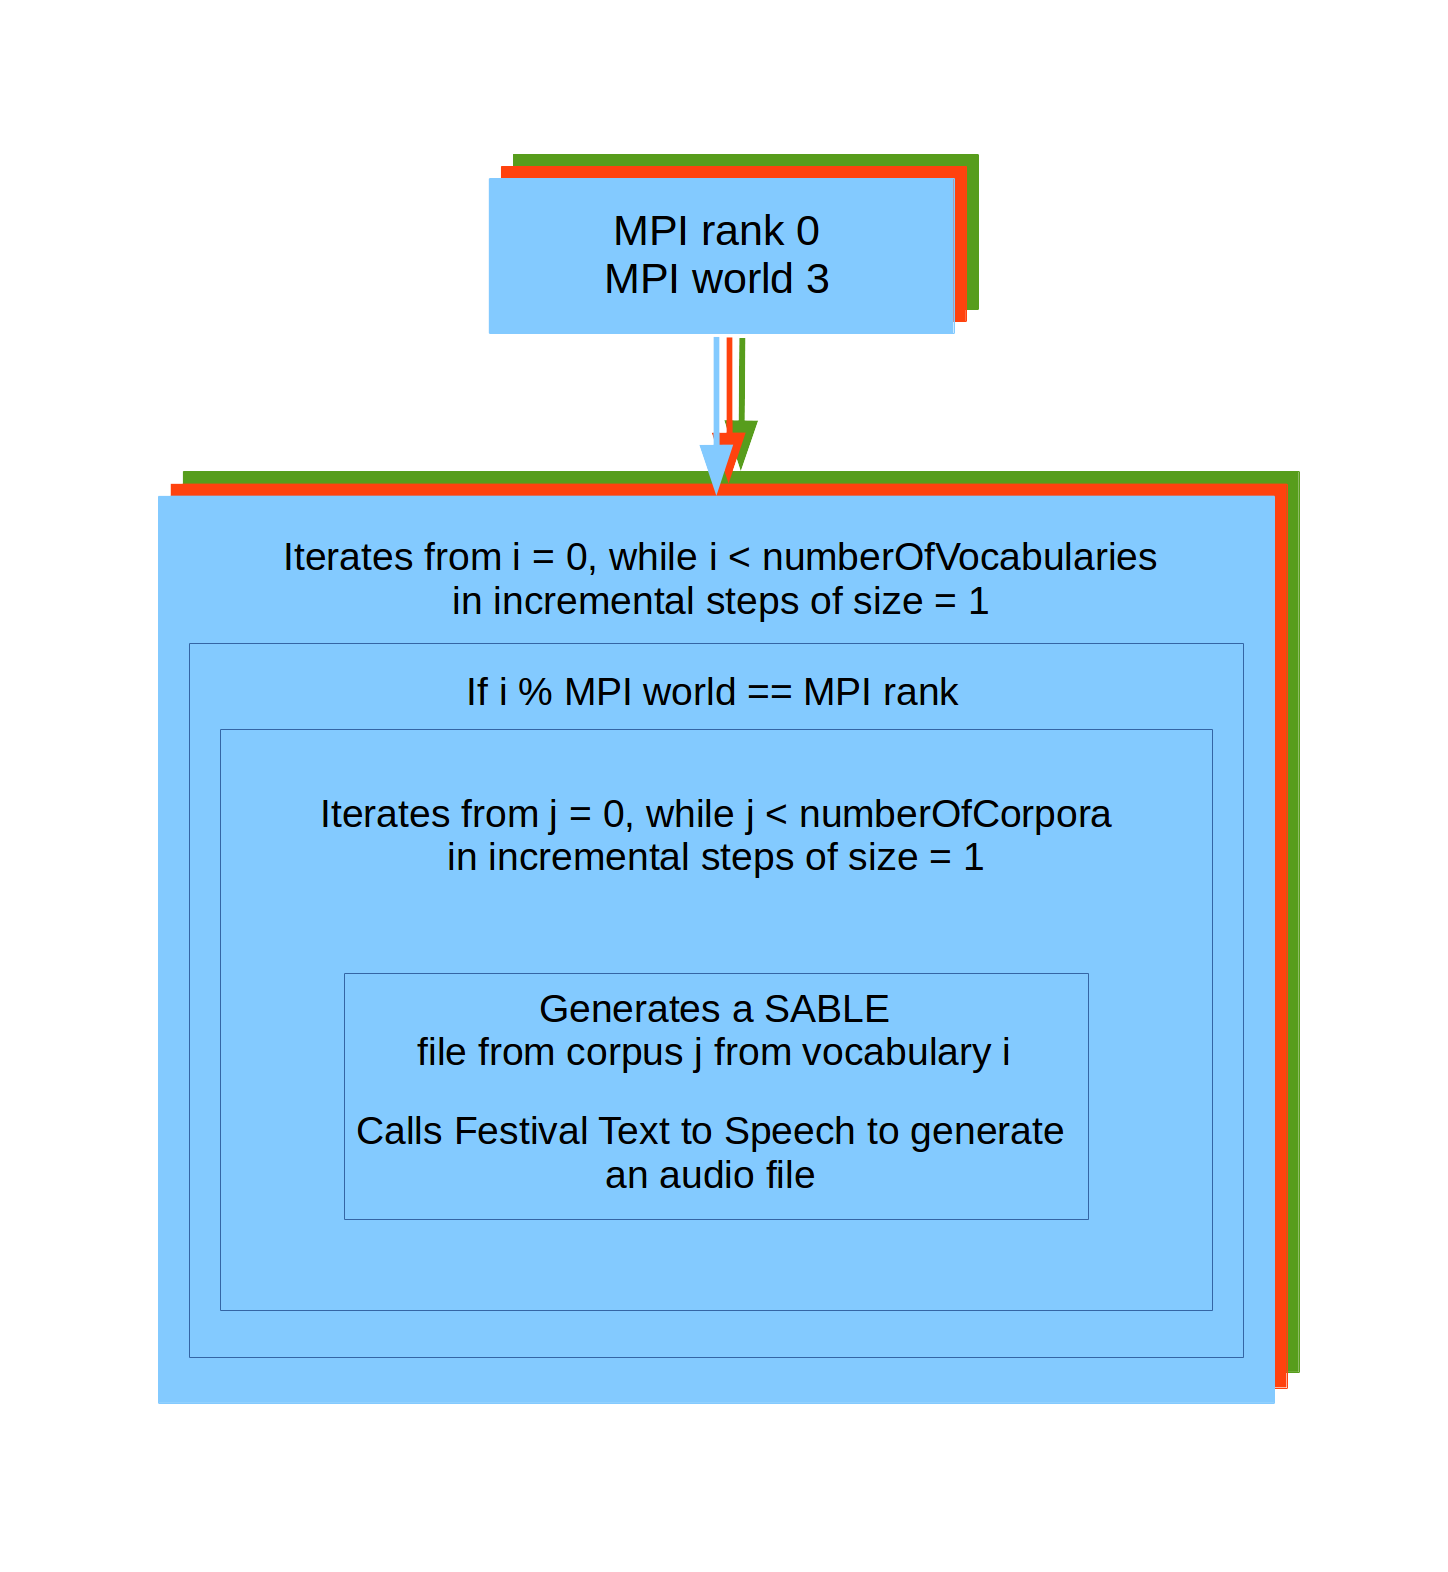
\includegraphics[width=0.49\linewidth]{Corpora_Generation_ALG.png}}
    \hfill
  \subfloat[Each \gls{mpi} rank will end up with a set of vocabularies to generate the corpora corresponding to such vocabularies (i.e. if we have 10 corpora per vocabulary, rank 0 will end up generating 40 corpora serially while ranks 1 and 2 will generate 30 corpora each serially.\label{sub:CorporaGenerationParallelization}]{%
        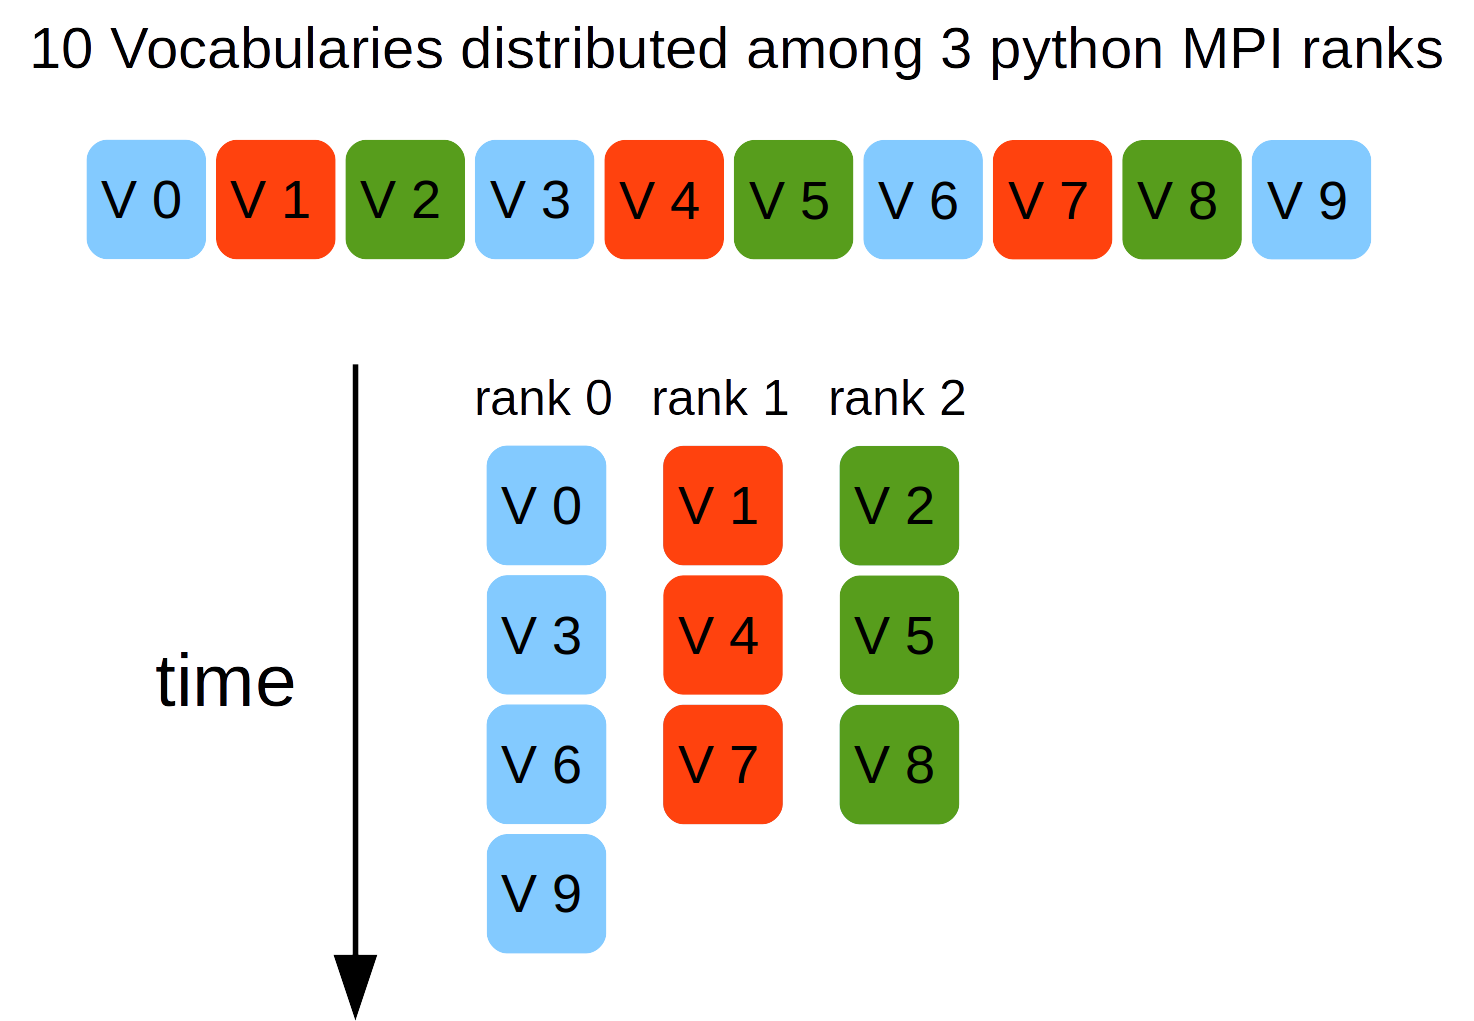
\includegraphics[width=0.49\linewidth]{CorporaGenerationParallelization.png}}
	\caption{Parallelization scheme for the Corpora Generation Process. This is a distribution of corpora generation among Python \gls{mpi} ranks. The corpora generation tasks are distributed among Python \gls{mpi} ranks as a deck of cards is distributed among players.}
  \label{fig:CorporaGenerationParallelization} 
\end{figure*}

%\begin{figure}[h!]
    %\centering
    %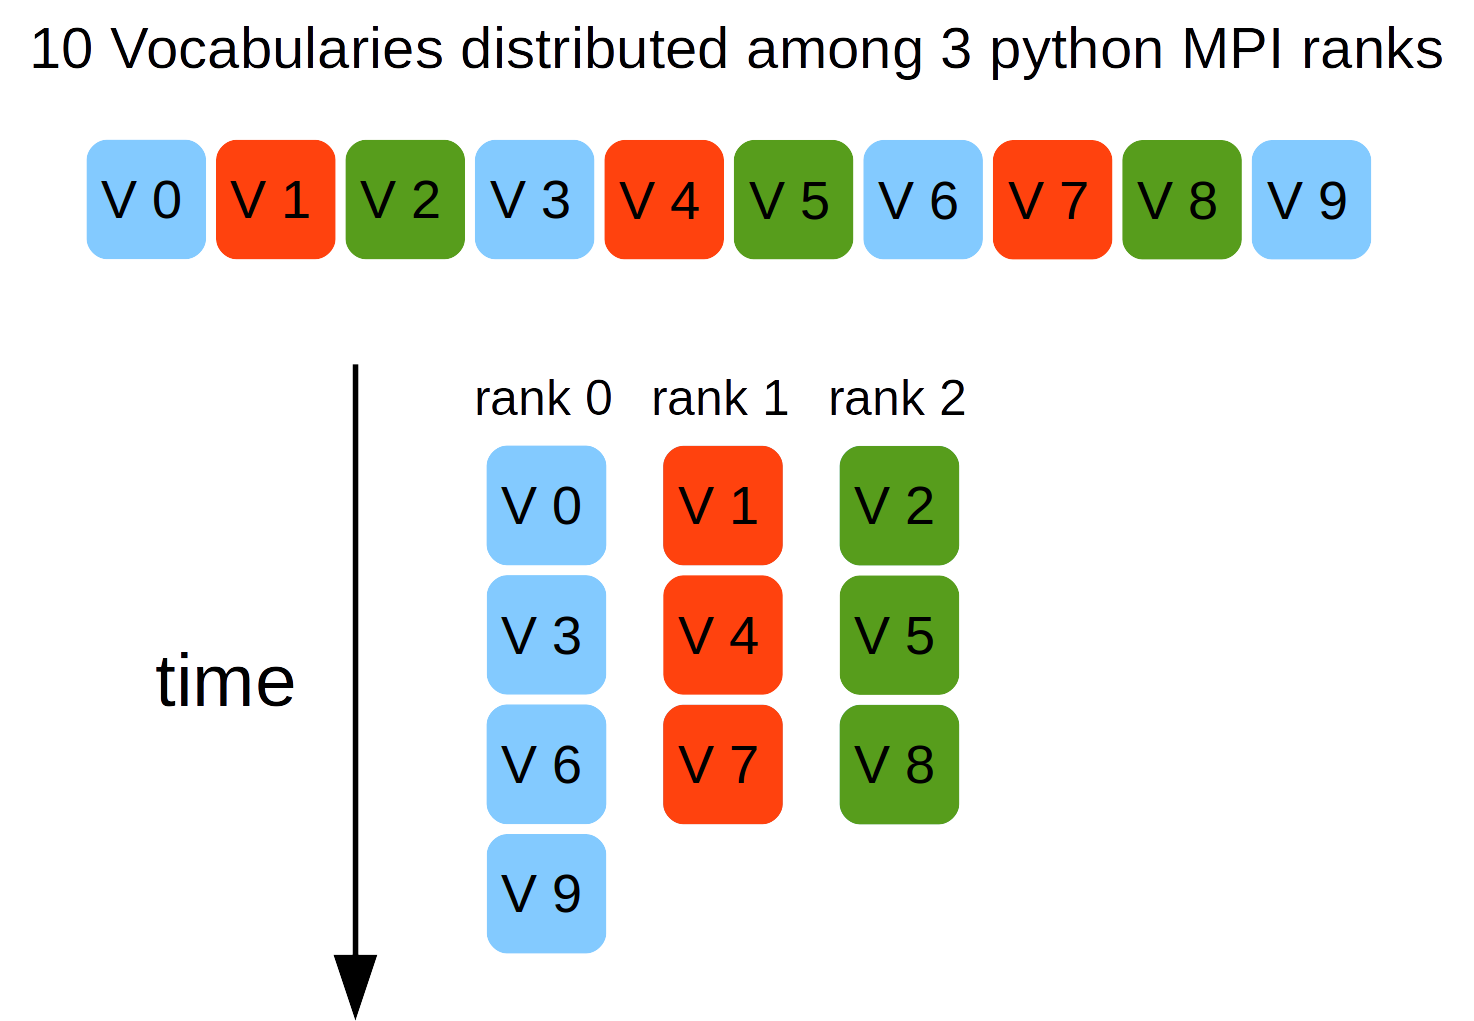
\includegraphics[width=0.4\textwidth]{CorporaGenerationParallelization.png}
    %\caption{Distribution of corpora generation among Python \gls{mpi} ranks. The corpora generation tasks are distributed among Python \gls{mpi} ranks as a deck of cards is distributed among players. Each \gls{mpi} rank will end up with a set of vocabularies to generate the corpora corresponding to such vocabularies (i.e. if we have 10 corpora per vocabulary, rank 0 will end up generating 40 corpora serially while ranks 1 and 2 will generate 30 corpora each serially.}
    %\label{fig:CorporaGenerationParallelization}
%\end{figure}



















\section{Results}

Parallel scalability is a measurement that indicates how efficient is a code when using an increasing number of parallel processing elements--Nodes or Processes and \glspl{cpu} or Threads--on a computational resource. There are two ways to measure the parallel performance of a given application. The measure to be applied will depend on whether the application is \gls{cpu}-bound or memory-bound. Such measurements are referred to as \emph{strong} and \emph{weak} scaling, respectively~\cite{noauthor_measuring_nodate}.
















\subsection{\glsfirst{el} Scaling Tests}

Fig. \ref{fig:EL_Strong_Scaling} shows the strong scaling capacity of our code in terms of run time vs. number of processing elements used for the task. In these tests we constrained the code to run one \gls{mpi} rank per Cooley node. Each \gls{mpi} rank spreads an specific number of threads through the different \glspl{cpu} in its corresponding node (Fig. \ref{fig:Encoder_Parallelization}). The problem size stays fixed but the number of processing elements are increased. Figs.~\ref{sub:EL_Strong_Scaling_Left} and~\ref{sub:EL_Strong_Scaling1_Left} show--at first--a good scaling capacity. This is supported by Figs.~\ref{sub:EL_Strong_Scaling_Right} and~\ref{sub:EL_Strong_Scaling1_Right}. Let $t_1$ be the amount of time to complete a work unit with $1$ processing element, and $t_N$ the amount of time to complete the same unit of work with $N$ processing elements, the Strong Scaling Efficiency shown in Figs.~\ref{sub:EL_Strong_Scaling_Right} and~\ref{sub:EL_Strong_Scaling1_Right} is: $t_1 / (N * t_N) * 100$.

\begin{figure*}[tb] 
    \centering
  \subfloat[Run time vs. the number of nodes for different number of threads per node.\label{sub:EL_Strong_Scaling_Left}]{%
       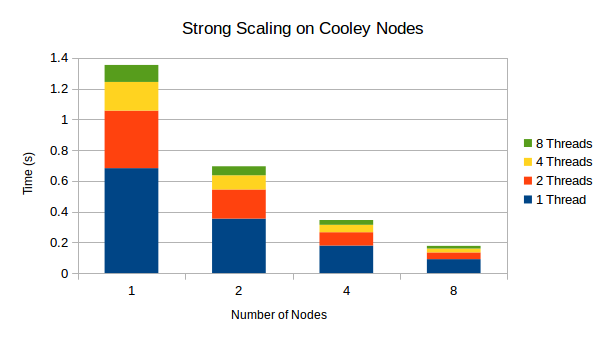
\includegraphics[width=0.49\linewidth]{EL_Strong_Scaling_Left.png}}
    \hfill
  \subfloat[Efficiency vs. the number of nodes for different numbers of threads per node.\label{sub:EL_Strong_Scaling_Right}]{%
        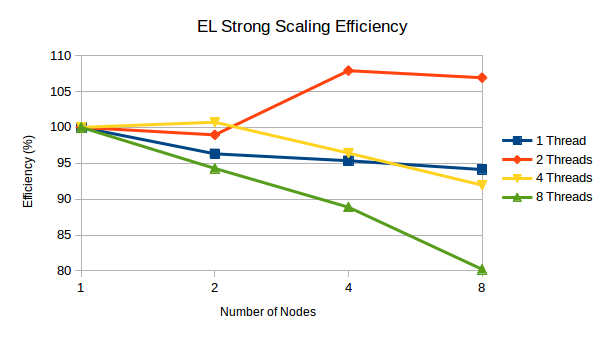
\includegraphics[width=0.49\linewidth]{EL_Strong_Scaling_Right.png}}
\\
  \subfloat[Run time vs. the number of nodes for different number of threads per node.\label{sub:EL_Strong_Scaling1_Left}]{%
       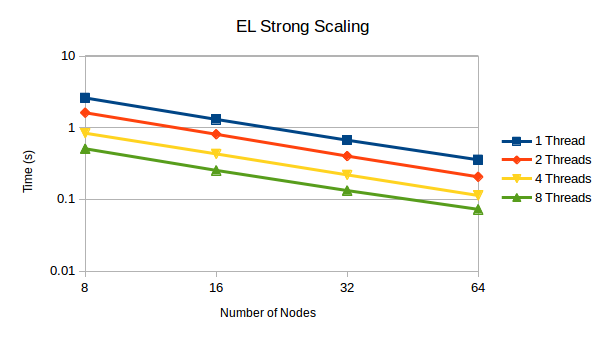
\includegraphics[width=0.49\linewidth]{EL_Strong_Scaling1_Left.png}}
    \hfill
    \subfloat[Efficiency vs. the number of nodes for different numbers of threads per node. Race line (reference) is taken at 8 computing nodes.\label{sub:EL_Strong_Scaling1_Right}]{%
        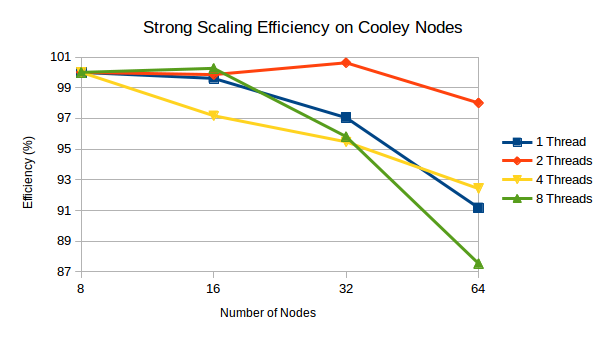
\includegraphics[width=0.49\linewidth]{EL_Strong_Scaling1_Right.png}}
	\caption{Strong scaling tests of the \gls{el} algorithm on Cooley nodes. Each \gls{mpi} rank runs in a different node with 1, 2, 4 and 8 \gls{omp} threads running in each rank.}
  \label{fig:EL_Strong_Scaling} 
\end{figure*}

%\begin{figure}[h!]
    %\centering
    %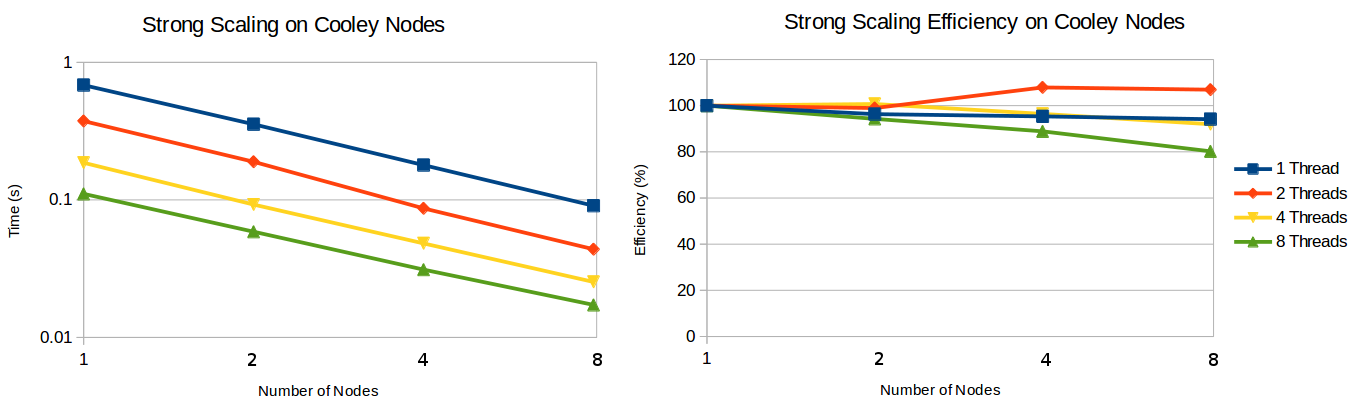
\includegraphics[width=0.5\textwidth]{Strong_Scaling.png}
    %\caption{Strong scaling tests on Cooley nodes. Left: Strong scaling. Run time vs. the number of nodes for different number of threads per node. The problem size stays fixed but the number of processing elements are increased. Straight lines in logarithmic scales indicates good scaling capacity. Right: Strong scaling efficiency vs. the number of nodes for different numbers of threads per node. Let $t_1$ be the amount of time to complete a work unit with 1 processing element, and $t_N$ the amount of time to complete the same unit of work with $N$ processing elements, the Strong Scaling Efficiency is: $t_1 / (N * t_N) * 100$.}
    %\label{fig:Strong_Scaling}
%\end{figure}

For the tests shown in Figs.~\ref{sub:EL_Strong_Scaling_Left} and~\ref{sub:EL_Strong_Scaling_Right} we generated an \gls{el} whose specifications are shown in Table~\ref{Medium_Model}, while for the tests shown in Figs.~\ref{sub:EL_Strong_Scaling1_Left} and~\ref{sub:EL_Strong_Scaling1_Right} we generated an \gls{el} whose specifications are shown in Table~\ref{Big_Model}.

\begin{table*}[tb]
\centering
\caption{\gls{el} of normal size to test strong scaling on 1, 2, 4 and 8 computing nodes. The different \glspl{rf}, percentages and dimensionalities are explained in~\cite{Dematties2018}.}
%\resizebox{\columnwidth}{!}{%
\begin{tabular}{|c|l|l|l|l|l|l|l|}
\hline
Model  & \multicolumn{1}{c|}{\begin{tabular}[c]{@{}c@{}}Number\\ of CCs\end{tabular}} & \multicolumn{1}{c|}{\begin{tabular}[c]{@{}c@{}}Afferent\\  RF\end{tabular}} & \multicolumn{1}{c|}{\begin{tabular}[c]{@{}c@{}}Afferent\\ \%\end{tabular}} & \multicolumn{1}{c|}{\begin{tabular}[c]{@{}c@{}}Lateral\\ RF\end{tabular}} & \multicolumn{1}{c|}{\begin{tabular}[c]{@{}c@{}}Lateral\\ \%\end{tabular}} & \multicolumn{1}{c|}{\begin{tabular}[c]{@{}c@{}}Population\\ Dimensionality\end{tabular}} & \multicolumn{1}{c|}{\begin{tabular}[c]{@{}c@{}}Potential\\ \%\end{tabular}} \\ \hline
Normal & 23 x 23                                                                      & 5 x 127                                                                      & 5\%                                                                        & 9 x 9                                                                     & 90\%                                                                      & 15 x 15                                                                                  & 3\%                                                                         \\ \hline
\end{tabular}%}
\label{Medium_Model}
\end{table*}

Firstly, the \gls{el} tested in Figs.~\ref{sub:EL_Strong_Scaling_Left} and~\ref{sub:EL_Strong_Scaling_Right} has 529 \glspl{cc}. In order to avoid scaling efficiency degradation, the \gls{el} has to keep certain number of \glspl{cc} per \gls{omp} thread. The worst case in Fig.~\ref{sub:EL_Strong_Scaling_Left} is for 8 nodes running 8 threads each (i.e. 64 threads). In such case we ended up having approximately 8.2 \glspl{cc} per \gls{omp} thread. As can be seen in Fig.~\ref{sub:EL_Strong_Scaling_Right} the strong scaling efficiency was never below 80\%. 

Since our computational model is intended to be run on leadership supercomputers--such as Theta at \gls{alcf}--in the future, it was necessary to test the Strong Scaling Efficiency of this on more computing nodes at Cooley. Specifically, we wanted to test the behaviour of the scaling running on up to 64 nodes with 8 \gls{omp} threads each since the more nodes you incorporate, the more \gls{ipc} load you have. In order to keep a considerable number of computing nodes per \gls{omp} thread we generated an \gls{el} with the specifications shown in Table~\ref{Big_Model}. 

\begin{table*}[tb]
\centering
\caption{\gls{el} of large size to test strong scaling on 8, 16, 32 and 64 computing nodes. The different \glspl{rf}, percentages and dimensionalities are explained in~\cite{Dematties2018}.}
%\resizebox{\columnwidth}{!}{%
\begin{tabular}{|c|l|l|l|l|l|l|l|}
\hline
Model  & \multicolumn{1}{c|}{\begin{tabular}[c]{@{}c@{}}Number\\ of CCs\end{tabular}} & \multicolumn{1}{c|}{\begin{tabular}[c]{@{}c@{}}Afferent\\  RF\end{tabular}} & \multicolumn{1}{c|}{\begin{tabular}[c]{@{}c@{}}Afferent\\ \%\end{tabular}} & \multicolumn{1}{c|}{\begin{tabular}[c]{@{}c@{}}Lateral\\ RF\end{tabular}} & \multicolumn{1}{c|}{\begin{tabular}[c]{@{}c@{}}Lateral\\ \%\end{tabular}} & \multicolumn{1}{c|}{\begin{tabular}[c]{@{}c@{}}Population\\ Dimensionality\end{tabular}} & \multicolumn{1}{c|}{\begin{tabular}[c]{@{}c@{}}Potential\\ \%\end{tabular}} \\ \hline
Big & 128 x 128                                                                      & 5 x 127                                                                      & 5\%                                                                        & 9 x 9                                                                     & 90\%                                                                      & 15 x 15                                                                                  & 3\%                                                                         \\ \hline
\end{tabular}%}
\label{Big_Model}
\end{table*}

This model has 16384 \glspl{cc} and for the worst case in which there are 64 computing nodes with 8 \gls{omp} threads each (512 threads) the model ended up distributing 32 \glspl{cc} per \gls{omp} thread. Each \gls{cc} in this model has 225 neural units to reach a total of 3686400 neural units. Each neural unit has 31 proximal (afferent) synapses and 432 distal (lateral) synapses to reach a total of 1706803200 synapses in the \gls{el}. Given the size of this model we could not run experiments from 1, 2 nor 4 computing nodes since the amount of time a simulation of such characteristics could take far exceeded the time provided by \texttt{qsub} command on Cooley. So we started the tests from 8 computing nodes for 1, 2, 4 and 8 \gls{omp} threads as shown in Fig.~\ref{sub:EL_Strong_Scaling1_Left}.

%\begin{figure*}[tb] 
    %\centering
  %\subfloat[Run time vs. the number of nodes for different number of threads per node.\label{sub:EL_Strong_Scaling1_Left}]{%
       %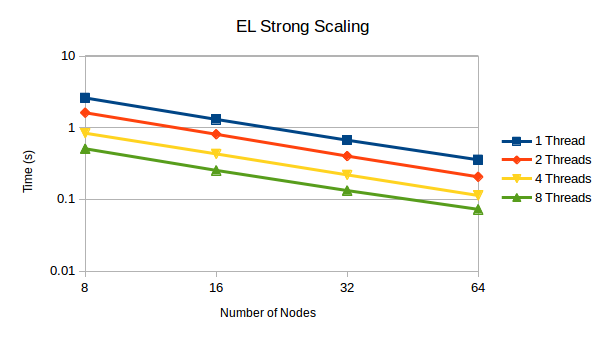
\includegraphics[width=0.49\linewidth]{EL_Strong_Scaling1_Left.png}}
    %\hfill
  %\subfloat[Efficiency vs. the number of nodes for different numbers of threads per node.\label{sub:EL_Strong_Scaling1_Right}]{%
        %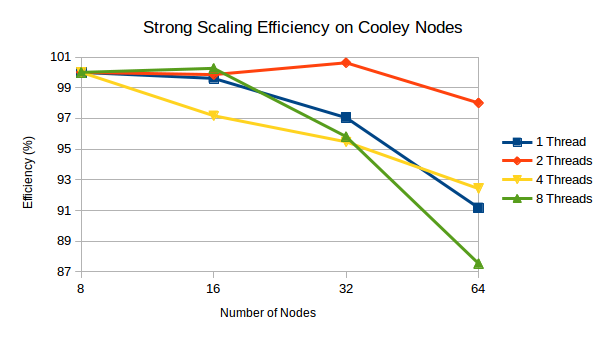
\includegraphics[width=0.49\linewidth]{EL_Strong_Scaling1_Right.png}}

  %\caption{Strong scaling tests on Cooley nodes. Reference is taken from 8 computing nodes ahead.}
  %\label{fig:EL_Strong_Scaling1} 
%\end{figure*}


%\begin{figure}[h!]
    %\centering
    %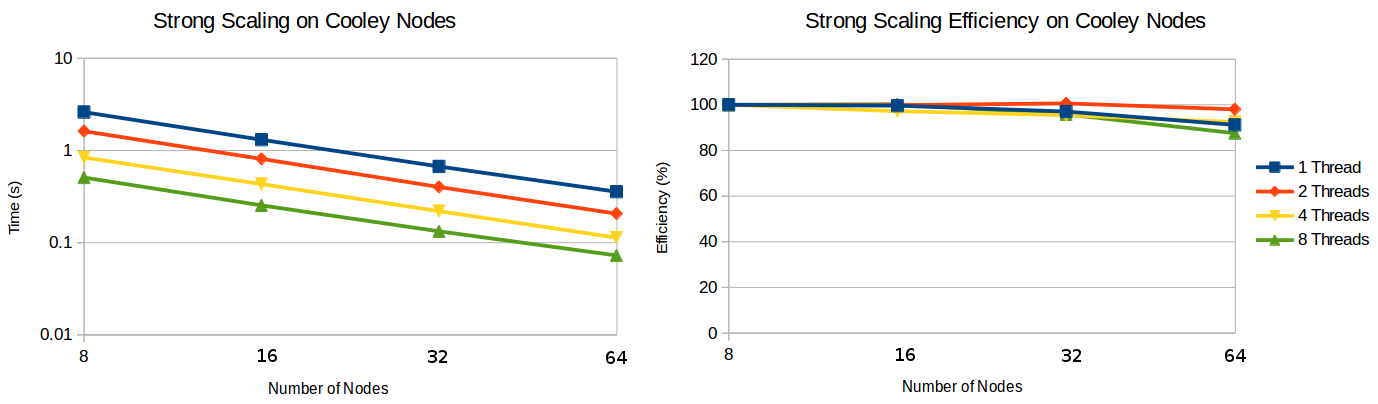
\includegraphics[width=0.5\textwidth]{Strong_Scaling1.png}
    %\caption{Strong scaling tests on Cooley nodes. Left: Strong scaling. Run time vs. the number of nodes for different number of threads per node. The problem size stays fixed but the number of processing elements are increased. Straight lines in logarithmic scales indicates good scaling capacity. Right: Strong scaling efficiency vs. the number of nodes for different numbers of threads per node. Let $t_1$ be the amount of time to complete a work unit with 1 processing element, and $t_N$ the amount of time to complete the same unit of work with $N$ processing elements, the Strong Scaling Efficiency is: $t_1 / (N * t_N) * 100$.}
    %\label{fig:Strong_Scaling1}
%\end{figure}

As can be seen in Fig.~\ref{sub:EL_Strong_Scaling1_Right}, the larger amount of compute nodes (\gls{mpi} ranks) with the consequent growth of \gls{mpi} \gls{ipc} load did not affect the strong scaling efficiency of the model which was well above the 85\%.

In reference to Weak Scaling, in order to keep the number of \glspl{cc} per \gls{omp} thread ratio constant we used the \glspl{el} detailed in the Table~\ref{Weak_Scaling_Models}. For all the cases detailed in the table, the ratio of \glspl{cc} per \gls{omp} thread was 32.

\begin{table*}[tb]
\centering
\caption{\glspl{el} of different sizes to test weak scaling on 1, 2, 4, 8, 16, 32 and 64 computing nodes. The different \glspl{rf}, percentages and dimensionalities are explained in~\cite{Dematties2018}.}
%\resizebox{\columnwidth}{!}{%
\begin{tabular}{|c|c|c|c|c|c|c|c|}
\hline
\begin{tabular}[c]{@{}c@{}}Number of\\ Nodes\end{tabular} & \begin{tabular}[c]{@{}c@{}}Number\\ of CCs\end{tabular} & \begin{tabular}[c]{@{}c@{}}Afferent\\  RF\end{tabular} & \begin{tabular}[c]{@{}c@{}}Afferent\\ \%\end{tabular} & \begin{tabular}[c]{@{}c@{}}Lateral\\ RF\end{tabular} & \begin{tabular}[c]{@{}c@{}}Lateral\\ \%\end{tabular} & \begin{tabular}[c]{@{}c@{}}Population\\ Dimensionality\end{tabular} & \begin{tabular}[c]{@{}c@{}}Potential\\ \%\end{tabular} \\ \hline
1 Node                                                    & 16 x 16                                                 & 5 x 127                                                 & 5\%                                                   & 9 x 9                                                & 90\%                                                 & 15 x 15                                                             & 3\%                                                    \\ \hline
2 Nodes                                                   & 16 x 32                                                 & 5 x 127                                                 & 5\%                                                   & 9 x 9                                                & 90\%                                                 & 15 x 15                                                             & 3\%                                                    \\ \hline
4 Nodes                                                   & 32 x 32                                                 & 5 x 127                                                 & 5\%                                                   & 9 x 9                                                & 90\%                                                 & 15 x 15                                                             & 3\%                                                    \\ \hline
8 Nodes                                                   & 32 x 64                                                 & 5 x 127                                                 & 5\%                                                   & 9 x 9                                                & 90\%                                                 & 15 x 15                                                             & 3\%                                                    \\ \hline
16 Nodes                                                  & 64 x 64                                                 & 5 x 127                                                 & 5\%                                                   & 9 x 9                                                & 90\%                                                 & 15 x 15                                                             & 3\%                                                    \\ \hline
32 Nodes                                                  & 64 x 128                                                & 5 x 127                                                 & 5\%                                                   & 9 x 9                                                & 90\%                                                 & 15 x 15                                                             & 3\%                                                    \\ \hline
64 Nodes                                                  & 128 x 128                                               & 5 x 127                                                 & 5\%                                                   & 9 x 9                                                & 90\%                                                 & 15 x 15                                                             & 3\%                                                    \\ \hline
\end{tabular}%}
\label{Weak_Scaling_Models}
\end{table*}

Fig.~\ref{fig:EL_Weak_Scaling} shows the weak scaling performance of the model. In this case the problem workload assigned to each processing element stays constant and additional elements are used to solve a larger total problem (i.e. a problem that would not fit in the available RAM on a single node). The bars in Fig.~\ref{sub:EL_Weak_Scaling_Left} shows--at first--a good scenario. As can be seen in Fig.~\ref{sub:EL_Weak_Scaling_Right}, the scaling efficiency was always above the 75\%. Let $t_1$ be the amount of time to complete a work unit with $1$ processing element, and $t_N$ the amount of time to complete $N$ times the same unit of work with $N$ processing elements, the Weak Scaling Efficiency is: $t_1 / t_N * 100$. This measures show that the model parallel execution is not affected by \gls{mpi} \gls{ipc} load as the number of computing nodes increases. This scenario is specially evident for the case of one \gls{omp} thread in whose case the worst efficiency is over the 95\%.

\begin{figure*}[tb] 
    \centering
  \subfloat[Run time vs. the number of nodes for different number of threads per node.\label{sub:EL_Weak_Scaling_Left}]{%
       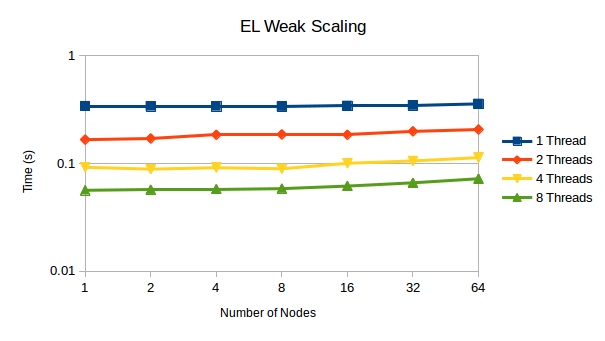
\includegraphics[width=0.49\linewidth]{EL_Weak_Scaling_Left.png}}
    \hfill
  \subfloat[Efficiency vs. the number of nodes for different numbers of threads per node.\label{sub:EL_Weak_Scaling_Right}]{%
        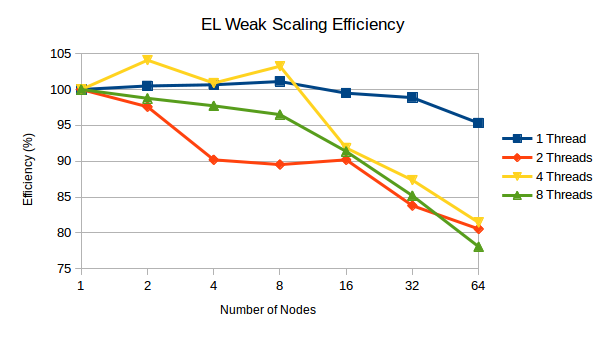
\includegraphics[width=0.49\linewidth]{EL_Weak_Scaling_Right.png}}

	\caption{Weak scaling tests of the \gls{el} algorithm on Cooley nodes. Each \gls{mpi} rank runs in a different node with 1, 2, 4 and 8 \gls{omp} threads running in each rank.}
  \label{fig:EL_Weak_Scaling} 
\end{figure*}


%\begin{figure}[h!]
    %\centering
    %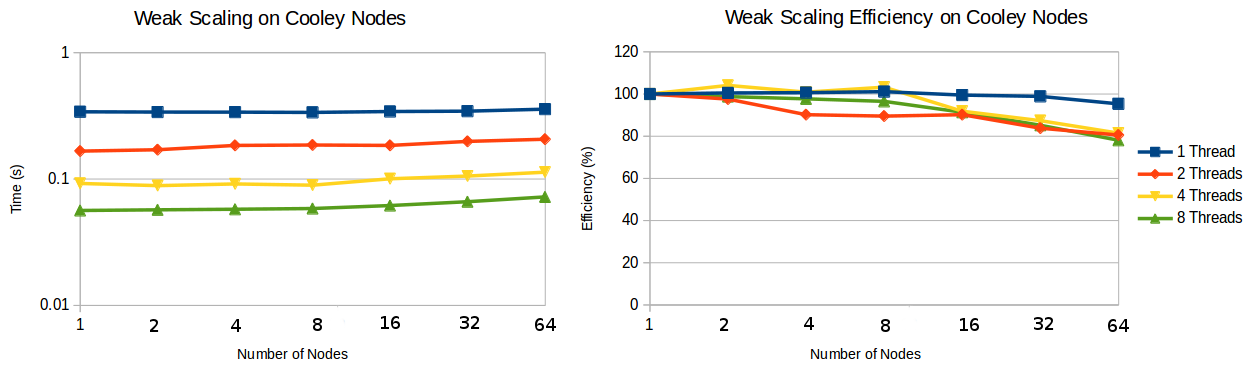
\includegraphics[width=0.5\textwidth]{Weak_Scaling.png}
    %\caption{Weak scaling tests on Cooley nodes. Left: Weak scaling. Run time vs. the number of nodes for different number of threads per node. In this case the problem workload assigned to each processing element stays constant and additional elements are used to solve a larger total problem (i.e. a problem that would not fit in the available RAM on a single node). Right: Weak scaling efficiency vs. the number of nodes for different numbers of threads per node. Let $t_1$ be the amount of time to complete a work unit with 1 processing element, and $t_N$ the amount of time to complete $N$ times the same unit of work with $N$ processing elements, the Weak Scaling Efficiency is: $t_1 / t_N * 100$.}
    %\label{fig:Weak_Scaling}
%\end{figure}

Figs.~\ref{sub:EL_Strong_Scaling_Left} and~\ref{sub:EL_Strong_Scaling1_Left} show an initially good strong scalability of our code while Fig. \ref{sub:EL_Weak_Scaling_Left} allows us to foresee a good weak scaling performance in high end leadership supercomputers too. All those visual results are supported by good measures of efficiency.






















\subsection{\glsfirst{mrstsa} Scaling Tests}
\label{MRSTSA_Scaling_Tests}

We tested the scaling capacity of this code on Cooley nodes. In terms of Strong scaling, we run the algorithm in order to process 64 corpora--one corpus per vocabulary. Fig.~\ref{sub:MRSTSA_Strong_Scaling} shows a really good scaling of this code. The problem size stays fixed--64 corpora processing by means of \gls{mrstsa} algorithm--but the number of processing elements are increased.

\begin{figure*}[tb] 
    \centering
  \subfloat[Run time vs. the number of nodes for different number of threads per node.\label{sub:MRSTSA_Strong_Scaling}]{%
       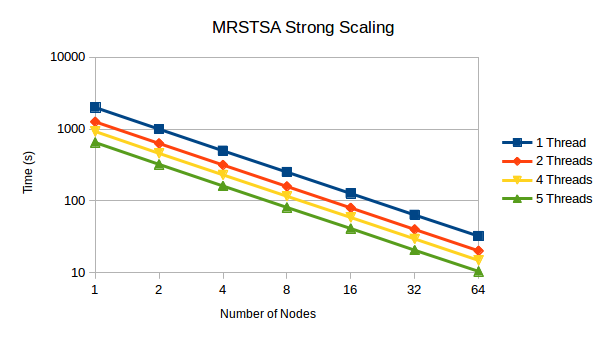
\includegraphics[width=0.49\linewidth]{MRSTSA_Strong_Scaling.png}}
    \hfill
  \subfloat[Run time vs. the number of nodes for 5 threads per node.\label{sub:MRSTSA_Weak_Scaling}]{%
        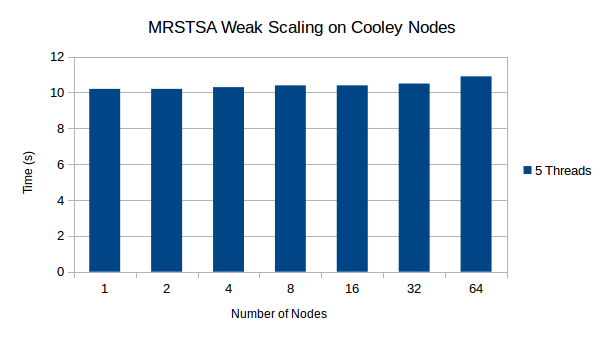
\includegraphics[width=0.49\linewidth]{MRSTSA_Weak_Scaling.png}}
\\
  \subfloat[Efficiency vs. the number of nodes for different number of threads per node.\label{sub:MRSTSA_Strong_Scaling_Efficiency}]{%
       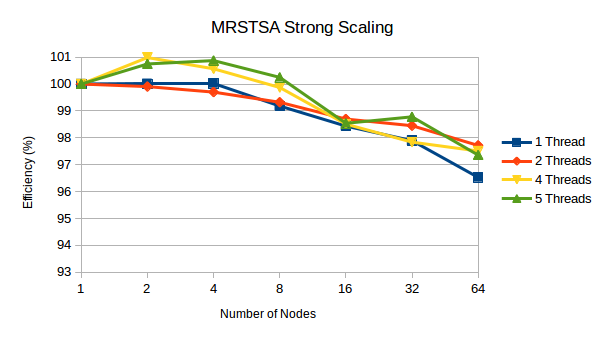
\includegraphics[width=0.49\linewidth]{MRSTSA_Strong_Scaling_Efficiency.png}}
    \hfill
  \subfloat[Efficiency vs. the number of nodes for 5 threads per node.\label{sub:MRSTSA_Weak_Scaling_Efficiency}]{%
        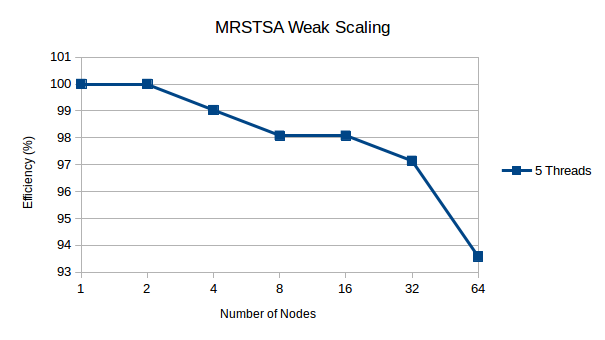
\includegraphics[width=0.49\linewidth]{MRSTSA_Weak_Scaling_Efficiency.png}}
	\caption{Strong and Weak scaling tests of the \gls{mrstsa} algorithm on Cooley nodes. Each \gls{mpi} rank runs in a different node with 1, 2, 4 and 5 \gls{omp} threads running in each rank.}
  \label{fig:MRSTSA_Scaling} 
\end{figure*}

%\begin{figure}[h!]
    %\centering
    %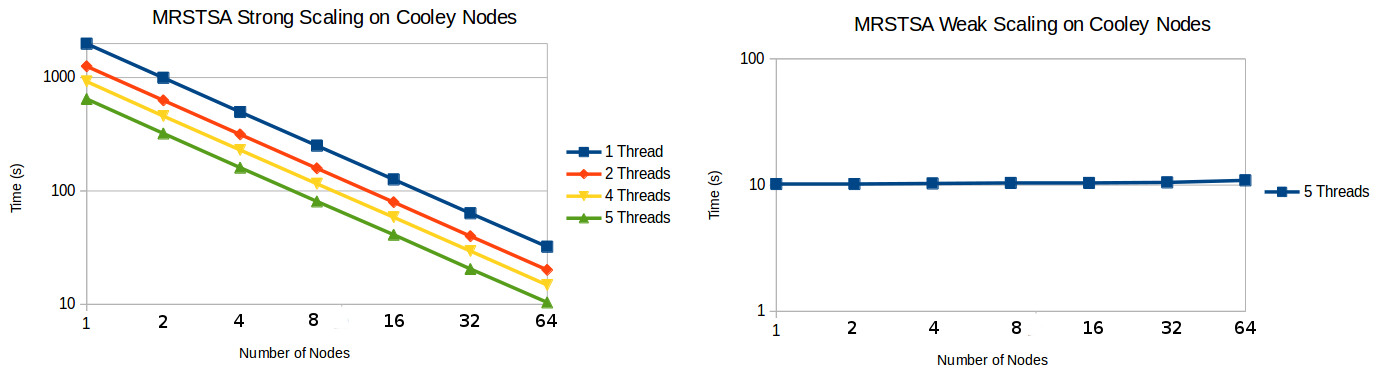
\includegraphics[width=0.5\textwidth]{MRSTSA_Scaling.png}
    %\caption{Strong and Weak scaling tests on Cooley nodes. Left: Strong scaling. Run time vs. the number of nodes for different number of threads per node. The problem size stays fixed--64 corpora processing by means of \gls{mrstsa} algorithm--but the number of processing elements are increased. Right: Weak scaling. Run time vs. the number of nodes for 5 threads per node. In this case the problem workload assigned to each processing element stays constant and additional elements are used to solve a larger total problem (i.e. we add more corpora for process as the number of nodes increases in such a way that each node has to process only one corpora).}
    %\label{fig:MRSTSA_Scaling}
%\end{figure}

Each process run in a different node. We use a number of \gls{omp} threads which ranges from 1 to 5. Five is the number of spectral components in the \gls{mrstsa} algorithm~\cite{Dematties2018}. Another issue to take into account is that in order to make this code scale in the way showed by the chart, all the corpora have to have the same size, otherwise--and since the code distributes corporas on different processes in static way--some processes which take over smaller corpora would finish before other processes that take over larger corpora producing considerable load imbalance in the \gls{mpi} environment. We have to think in a way to make the distribution of corpora on processes dynamic--such as \gls{omp} dynamic schedule. Nevertheless, trying to balance the load among the different \gls{mpi} ranks could produce a severe degradation of Efficiency originated in the increased load of \gls{ipc} that such techniques require~\cite{hu2012biophysically}.

In reference to Weak scaling, we processed one corpus per \gls{mpi} rank by means of the obvious strategy of processing one corpus for one \gls{mpi} rank, two corpora for two \gls{mpi} rank, four corpora for four \gls{mpi} rank and so on. In Fig.~\ref{sub:MRSTSA_Weak_Scaling} the problem workload assigned to each processing element stays constant and additional elements are used to solve a larger total problem. We added more corpora per process as the number of nodes increases in such a way that each node has to process only one corpora. Fig.~\ref{sub:MRSTSA_Weak_Scaling} shows that this code scales very well in terms of weak scaling too.

Finally, Figs.~\ref{sub:MRSTSA_Strong_Scaling_Efficiency} and~\ref{sub:MRSTSA_Weak_Scaling_Efficiency} sustains the behavior of the charts with Strong Scaling Efficiencies well above the 96\% and Weak Scaling Efficiencies above the 93\%.

%\begin{figure*}[tb] 
    %\centering
  %\subfloat[Efficiency vs. the number of nodes for different number of threads per node.\label{sub:MRSTSA_Strong_Scaling_Efficiency}]{%
       %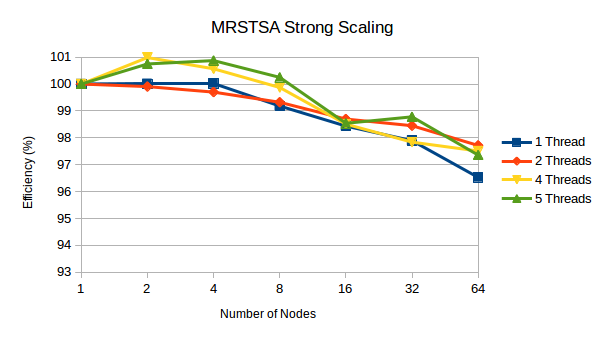
\includegraphics[width=0.49\linewidth]{MRSTSA_Strong_Scaling_Efficiency.png}}
    %\hfill
  %\subfloat[Efficiency vs. the number of nodes for 5 threads per node.\label{sub:MRSTSA_Weak_Scaling_Efficiency}]{%
        %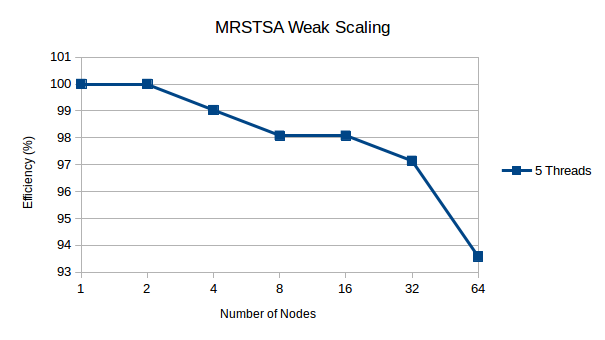
\includegraphics[width=0.49\linewidth]{MRSTSA_Weak_Scaling_Efficiency.png}}

  %\caption{Strong and Weak scaling efficiency on Cooley nodes.}
  %\label{fig:MRSTSA_Scaling_Efficiency} 
%\end{figure*}

%\begin{figure}[h!]
    %\centering
    %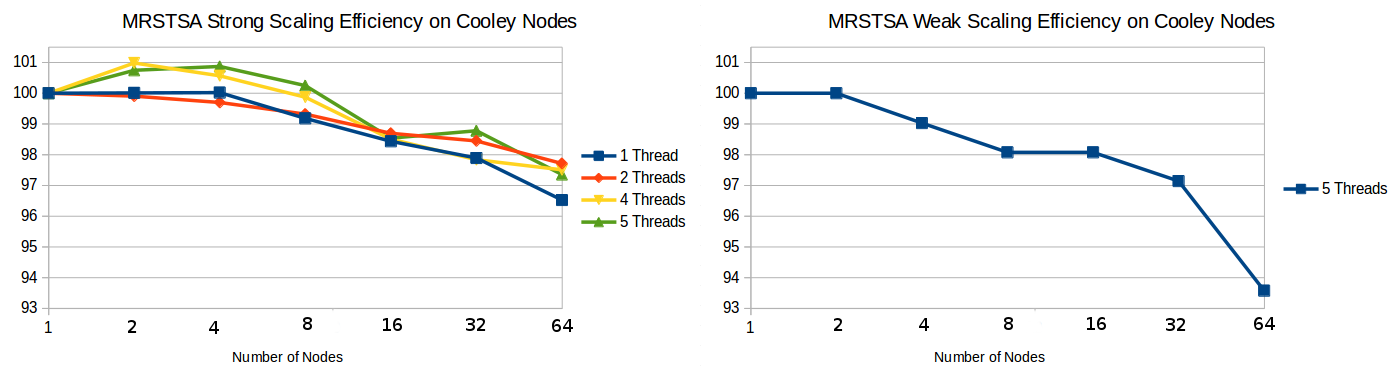
\includegraphics[width=0.5\textwidth]{MRSTSA_Scaling_Efficiency.png}
    %\caption{Strong and Weak scaling efficiency on Cooley nodes. Left: Strong scaling efficiency. Efficiency vs. the number of nodes for different number of threads per node. Let $t_1$ be the amount of time to complete a work unit with 1 processing element, and $t_N$ the amount of time to complete the same unit of work with $N$ processing elements, the Strong Scaling Efficiency is: $t_1 / (N * t_N) * 100$. Right: Weak scaling efficiency. Efficiency vs. the number of nodes for 5 threads per node. Let $t_1$ be the amount of time to complete a work unit with 1 processing element, and $t_N$ the amount of time to complete $N$ times the same unit of work with $N$ processing elements, the Weak Scaling Efficiency is: $t_1 / t_N * 100$.}
    %\label{fig:MRSTSA_Scaling_Efficiency}
%\end{figure}
















\subsection{Corpora Generation Scaling Tests}

In terms of Strong and Weak scaling (Fig.~\ref{fig:Corpora_Scaling}), we ran the algorithm in order to create 64 corpora from 64 vocabularies--one corpus per vocabulary. The code generated 64 cross synthesizer SABLE text files and then called to Festival using \texttt{text2wav} script in order to generate the audio \texttt{wav} files which uttered the text in the SABLE files.

\begin{figure*}[tb] 
    \centering
  \subfloat[Run time vs. the number of \glspl{cpu}.\label{sub:Corpora_Strong_Scaling}]{%
       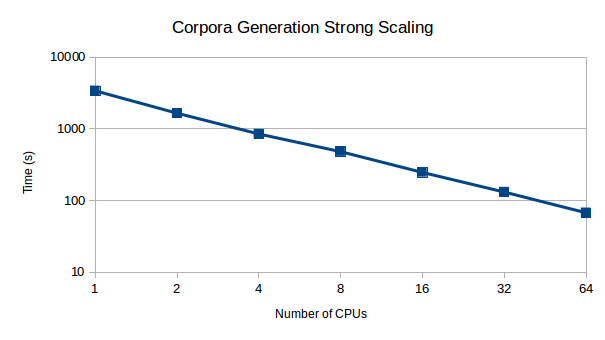
\includegraphics[width=0.49\linewidth]{Corpora_Strong_Scaling.png}}
    \hfill
  \subfloat[Run time vs. the number of \glspl{cpu}.\label{sub:Corpora_Weak_Scaling}]{%
	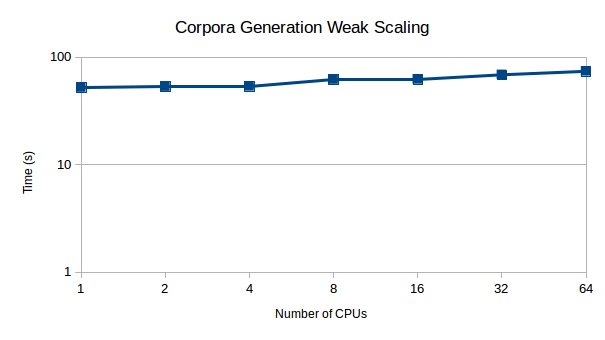
\includegraphics[width=0.49\linewidth]{Corpora_Weak_Scaling.png}}
\\
  \subfloat[Efficiency vs. the number of \glspl{cpu}.\label{sub:Corpora_Strong_Scaling_Efficiency}]{%
       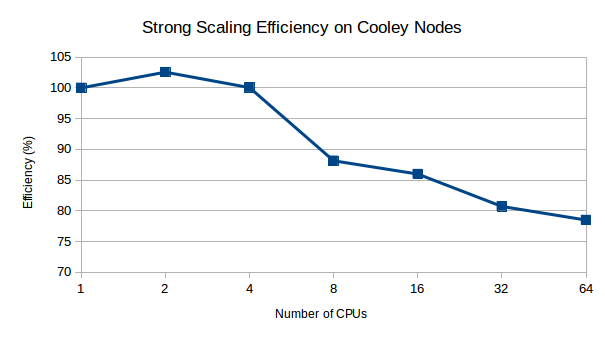
\includegraphics[width=0.49\linewidth]{Corpora_Strong_Scaling_Efficiency.png}}
    \hfill
  \subfloat[Efficiency vs. the number of \glspl{cpu}.\label{sub:Corpora_Weak_Scaling_Efficiency}]{%
	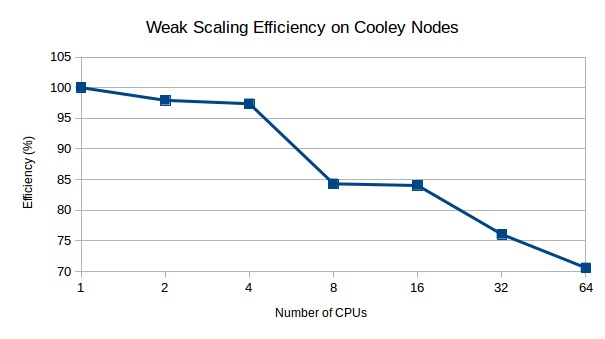
\includegraphics[width=0.49\linewidth]{Corpora_Weak_Scaling_Efficiency.png}}
	\caption{Strong and Weak scaling test of Corpora Generation on Cooley nodes. Each Python \gls{mpi} rank runs in a different \gls{cpu}. Since Cooley nodes have 12 \glspl{cpu} we had to ask for 2 nodes in order to run on 16 \glspl{cpu}, 3 nodes in order to run on 32 \glspl{cpu} and 6 nodes in order to run on 64 \glspl{cpu}.}
  \label{fig:Corpora_Scaling} 
\end{figure*}

%\begin{figure}[h!]
    %\centering
    %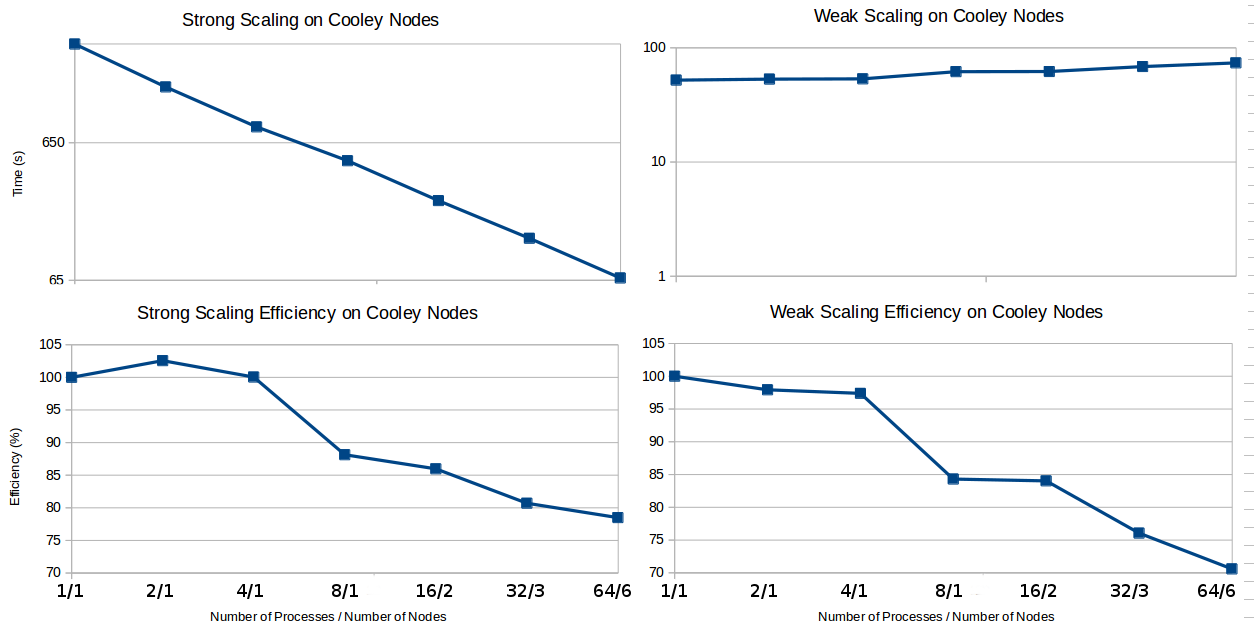
\includegraphics[width=0.5\textwidth]{CorporaGenerationScaling.png}
    %\caption{Strong and Weak scaling test on Cooley nodes. Left: Strong Scaling. Run time and Efficiency vs. the number of \glspl{cpu}. The problem size stays fixed, that is, the run has to generate 64 corpora. On the other hand the number of processing elements is increased from 1 to 64 \glspl{cpu} in powers of two. Right: Weak scaling. Run time and Efficiency vs. the number of \glspl{cpu}. In this case the problem workload assigned to each processing element stays constant and additional elements are used to solve a larger total problem (i.e. as we add more \glspl{cpu} we add more corpora in a way that one corpus is generated by \gls{cpu}). Since Cooley nodes have 12 \glspl{cpu} we had to ask for 2 nodes in order to run on 16 \glspl{cpu}, 3 nodes in order to run on 32 \glspl{cpu} and 6 nodes in order to run on 64 \glspl{cpu}.}
    %\label{fig:CorporaGenerationScaling}
%\end{figure}

Fig.~\ref{sub:Corpora_Strong_Scaling} shows a good strong scaling capacity of our code. As before, for strong scaling performance tests the problem size stays fixed, that is, the run has to generate 64 corpora. On the other hand the number of processing elements is increased from 1 to 64 \glspl{cpu} in powers of two. In this case we ran one \gls{mpi} rank per \gls{cpu}. Since one Cooley Node has 12 \glspl{cpu} we just needed 1 node in order to run 1, 2, 4 or 8 processes, 2 nodes (24 \glspl{cpu}) in order to run 16 processes, 3 nodes (36 \glspl{cpu}) in order to run 32 processes and finally 6 nodes (72 \glspl{cpu}) in order to run 64 processes.

%Nevertheless, we have to take into account that each process produces an independent set of corpora and does not need to transmit any data to other processes in the \gls{mpi} session. Then, we did not have \gls{ipc} issues in this code (this is pure parallelization, also called \emph{Embarrassingly parallel}~\cite{noauthor_embarrassingly_2018}).

Something to take into account is that to make this code scale in the way showed by the chart, all the corpora have to have the same size, otherwise--and since the code distributes corporas on different processes in static way--some processes which took over smaller corpora would have finished before other processes that took over larger corpora and would have wasted processing power waiting idly for other processes to finish. We have to think in a way to make the distribution of vocabularies on processes dynamic--such as \gls{omp} dynamic schedule. Nevertheless, trying to balance the load among the different \gls{mpi} ranks could produce a severe degradation of Efficiency originated in the increased \gls{ipc} load that such techniques require~\cite{hu2012biophysically}.

In Fig.~\ref{sub:Corpora_Strong_Scaling_Efficiency} we can see that the minimum Strong Scaling Efficiency is well above the 75\%.

In reference to Weak scaling (Fig.~\ref{sub:Corpora_Weak_Scaling})--as before--the problem workload assigned to each processing element stays constant and additional elements are used to solve a larger total problem (i.e. as we add more \glspl{cpu} we add more corpora in a way that one corpus is generated by \gls{cpu}). We generated one corpus per process using one corpus for one \gls{mpi} rank, two corpora for two \gls{mpi} ranks and so on. The bars shown in Fig.~\ref{sub:Corpora_Weak_Scaling} depict that this code scales well in terms of weak scaling too and--as Fig.~\ref{sub:Corpora_Weak_Scaling_Efficiency} shows--the Weak Scaling Efficiency of the code was never below the 70\%.










\section{Discussion}

In this paper we show how parallelization strategies with great independence on data coalescence scale efficiently on distributed memory systems while running biologically inspired computational models with highly sparse and random connectivity profiles.

Algorithmic implementations strongly based on \gls{simd} parallel computing architectures, impose important restrictions on memory data alignment. \gls{omp} threads in shared memory systems are instead highly independent and powerful processing abstractions which can perform complex task with eventual vectorization optimizations when possible.

Our findings show that the parallelization strategies used in this work present good and robust scaling efficiency even in front of intensive \gls{ipc} loads. Such behavior can be kept in a sustained manner as long as a minimum of balance in the computational load among different threads remains. In section~\ref{MRSTSA_Scaling_Tests} we showed very high scaling efficiencies. Yet, we warned about difficulties in front of a context with uneven corpus sizes. Achieving load balance in distributed memory systems is extremely expensive given the amount of \gls{ipc} overload needed. In this manner, we claim that the best way to balance computational load among computing elements is to try to confine as much computational load as possible in a shared memory unit without far exceeding the concurrent threading or hyperthreading capacity provided by a node. Once such conditions are satisfied it is relatively straightforward to spawn a bunch of threads in which the work could be distributed. Once in a shared memory system, \gls{omp} threads are much lighter that \gls{mpi} processes since threads do not duplicate heap nor program and they do not need complex communication methos to share data. Furthermore, \gls{omp} threads can manage load balancing efficiently and automatically since \gls{omp} manages dynamic parallel schedule for you. This is highly desirable specially in a simulation environment in which individual modules--such as \glspl{cc} in our cortical model--are not uniformly analogous in terms of size and or connectivity. In \gls{mpi} instead, the programmer has to deal with load balancing using intensive \gls{ipc} which is highly expensive especially when the communication is carried out among processes in different nodes. On the other side \gls{omp} threads suffer from false shearing in the \glspl{cpu} caches, but with a highly flexible parallelization scheme as the one used in section \ref{EL_Parallelization} the user can flexibly vary the parallelization granularity as to achieve the best performance avoiding that each thread exceeds the quota of cache memory available in each \gls{cpu}.

In Figs.~\ref{fig:EL_Strong_Scaling}, \ref{fig:EL_Weak_Scaling}, \ref{fig:MRSTSA_Scaling} and \ref{fig:Corpora_Scaling}, the phenomenon of \emph{superlinear-speedup} is present for several cases. In \cite{7733347} the authors pointed out that: \say{Mainly the superlinear speedup performance in persistent algorithms occurs due to the increased cache resources in the parallel computer architectures, the prefetching of shared variables in shared memory organization, or better scheduling in heterogeneous environments. The effects of the shared memory architectures also impact the performance behavior of the granular and scalable algorithms}. We absolutely endorse such statement and consider it sustainable as a general explanation for our case. Nevertheless, we also consider that more in depth analysis of memory utilization using profiling tools will be needed in the future.  

In section~\ref{EL_Parallelization} some problems could arise when a single \gls{cc} is too large to share a computing node with many others. If just 2 \glspl{cc} could fit in a node, the parallelization granularity would be very poor, but \gls{omp} is highly versatile and can easily manage nested threading. In such case we could vary the parallelization granularity in an extremely accessible manner with all the advantages of \gls{omp} in terms of dynamic load balancing. This nested parallelization strategy could be applied in section~\ref{MRSTSA_Scaling_Tests} in front of an eventual unbalanced computational load from an uneven corpora size distribution. 

This scenario in which the computational burden assigned to each shared memory system is distributed among a set of highly lightweight, flexible and dynamic \gls{omp} threads is really favorable in a context in which the number of \glspl{cpu} shearing memory increases specially in high-end supercomputers. In such respect and in front of the good results returned by our experiments we evaluate as viable the implementation of these parallelization strategies in high end supercomputers in the future.

We claim thus that this work introduces parallelization strategies whose flexibility and robustness are particularly useful in overly variable and biologically inspired computational scientific scenarios whose modelization approaches can vary dramatically in different biologically accurate implementations strategies in which there are erratic network structures with highly sparse and random connectivity profiles.













% An example of a floating figure using the graphicx package.
% Note that \label must occur AFTER (or within) \caption.
% For figures, \caption should occur after the \includegraphics.
% Note that IEEEtran v1.7 and later has special internal code that
% is designed to preserve the operation of \label within \caption
% even when the captionsoff option is in effect. However, because
% of issues like this, it may be the safest practice to put all your
% \label just after \caption rather than within \caption{}.
%
% Reminder: the "draftcls" or "draftclsnofoot", not "draft", class
% option should be used if it is desired that the figures are to be
% displayed while in draft mode.
%
%\begin{figure}[!t]
%\centering
%\includegraphics[width=2.5in]{myfigure}
% where an .eps filename suffix will be assumed under latex, 
% and a .pdf suffix will be assumed for pdflatex; or what has been declared
% via \DeclareGraphicsExtensions.
%\caption{Simulation results for the network.}
%\label{fig_sim}
%\end{figure}

% Note that the IEEE typically puts floats only at the top, even when this
% results in a large percentage of a column being occupied by floats.
% However, the Computer Society has been known to put floats at the bottom.


% An example of a double column floating figure using two subfigures.
% (The subfig.sty package must be loaded for this to work.)
% The subfigure \label commands are set within each subfloat command,
% and the \label for the overall figure must come after \caption.
% \hfil is used as a separator to get equal spacing.
% Watch out that the combined width of all the subfigures on a 
% line do not exceed the text width or a line break will occur.
%
%\begin{figure*}[!t]
%\centering
%\subfloat[Case I]{\includegraphics[width=2.5in]{box}%
%\label{fig_first_case}}
%\hfil
%\subfloat[Case II]{\includegraphics[width=2.5in]{box}%
%\label{fig_second_case}}
%\caption{Simulation results for the network.}
%\label{fig_sim}
%\end{figure*}
%
% Note that often IEEE papers with subfigures do not employ subfigure
% captions (using the optional argument to \subfloat[]), but instead will
% reference/describe all of them (a), (b), etc., within the main caption.
% Be aware that for subfig.sty to generate the (a), (b), etc., subfigure
% labels, the optional argument to \subfloat must be present. If a
% subcaption is not desired, just leave its contents blank,
% e.g., \subfloat[].


% An example of a floating table. Note that, for IEEE style tables, the
% \caption command should come BEFORE the table and, given that table
% captions serve much like titles, are usually capitalized except for words
% such as a, an, and, as, at, but, by, for, in, nor, of, on, or, the, to
% and up, which are usually not capitalized unless they are the first or
% last word of the caption. Table text will default to \footnotesize as
% the IEEE normally uses this smaller font for tables.
% The \label must come after \caption as always.
%
%\begin{table}[!t]
%% increase table row spacing, adjust to taste
%\renewcommand{\arraystretch}{1.3}
% if using array.sty, it might be a good idea to tweak the value of
% \extrarowheight as needed to properly center the text within the cells
%\caption{An Example of a Table}
%\label{table_example}
%\centering
%% Some packages, such as MDW tools, offer better commands for making tables
%% than the plain LaTeX2e tabular which is used here.
%\begin{tabular}{|c||c|}
%\hline
%One & Two\\
%\hline
%Three & Four\\
%\hline
%\end{tabular}
%\end{table}


% Note that the IEEE does not put floats in the very first column
% - or typically anywhere on the first page for that matter. Also,
% in-text middle ("here") positioning is typically not used, but it
% is allowed and encouraged for Computer Society conferences (but
% not Computer Society journals). Most IEEE journals/conferences use
% top floats exclusively. 
% Note that, LaTeX2e, unlike IEEE journals/conferences, places
% footnotes above bottom floats. This can be corrected via the
% \fnbelowfloat command of the stfloats package.




\section{Conclusion}

In this paper we showed a hybrid \gls{mpi}+\gls{omp} parallelization strategy which scales efficiently in a distributed memory system while running a computational approach inspired in the biology of mammalian cortex with a highly sparse and irregular connectivity profile. We showed this efficiency by means of strong and weak scaling tests at Cooley nodes.

Independence of data coalescence, flexible granularity reconfiguration, dynamically scheduled load balancing and lightweight parallel processing at shared memory parcels, configured salient features in our parallelization approach.

We consider such features of fundamental importance for the usage of this parallelization procedure in highly variable computational scientific scenarios with irregularly structured datasets typically found in biologically inspired research approaches.

By means of the results returned by this round of tests, we esteem this parallelization policy as viable to be used in high-end leadership supercomputers in the future.





% if have a single appendix:
%\appendix[Proof of the Zonklar Equations]
% or
%\appendix  % for no appendix heading
% do not use \section anymore after \appendix, only \section*
% is possibly needed

% use appendices with more than one appendix
% then use \section to start each appendix
% you must declare a \section before using any
% \subsection or using \label (\appendices by itself
% starts a section numbered zero.)
%


%\appendices
%\section{Proof of the First Zonklar Equation}
%Appendix one text goes here.

%% you can choose not to have a title for an appendix
%% if you want by leaving the argument blank
%\section{}
%Appendix two text goes here.


% use section* for acknowledgment
\ifCLASSOPTIONcompsoc
  % The Computer Society usually uses the plural form
  \section*{Acknowledgments}
\else
  % regular IEEE prefers the singular form
  \section*{Acknowledgment}
\fi


The authors would like to thank...


% Can use something like this to put references on a page
% by themselves when using endfloat and the captionsoff option.
\ifCLASSOPTIONcaptionsoff
  \newpage
\fi



% trigger a \newpage just before the given reference
% number - used to balance the columns on the last page
% adjust value as needed - may need to be readjusted if
% the document is modified later
%\IEEEtriggeratref{8}
% The "triggered" command can be changed if desired:
%\IEEEtriggercmd{\enlargethispage{-5in}}

% references section

% can use a bibliography generated by BibTeX as a .bbl file
% BibTeX documentation can be easily obtained at:
% http://mirror.ctan.org/biblio/bibtex/contrib/doc/
% The IEEEtran BibTeX style support page is at:
% http://www.michaelshell.org/tex/ieeetran/bibtex/
\bibliographystyle{IEEEtran}
% argument is your BibTeX string definitions and bibliography database(s)
\bibliography{IEEEabrv,bare_jrnl_compsoc}
%
% <OR> manually copy in the resultant .bbl file
% set second argument of \begin to the number of references
% (used to reserve space for the reference number labels box)
%\begin{thebibliography}{1}

%\bibitem{IEEEhowto:kopka}
%H.~Kopka and P.~W. Daly, \emph{A Guide to \LaTeX}, 3rd~ed.\hskip 1em plus
  %0.5em minus 0.4em\relax Harlow, England: Addison-Wesley, 1999.

%\end{thebibliography}

% biography section
% 
% If you have an EPS/PDF photo (graphicx package needed) extra braces are
% needed around the contents of the optional argument to biography to prevent
% the LaTeX parser from getting confused when it sees the complicated
% \includegraphics command within an optional argument. (You could create
% your own custom macro containing the \includegraphics command to make things
% simpler here.)
%\begin{IEEEbiography}[{\includegraphics[width=1in,height=1.25in,clip,keepaspectratio]{mshell}}]{Michael Shell}
% or if you just want to reserve a space for a photo:

\begin{IEEEbiography}[{\includegraphics[width=1in,height=1.25in,clip,keepaspectratio]{DarioDematties}}]{Dario Dematties}
is currently working toward a PhD degree in the Instituto de Ingenier\'ia Biom\'edica, Facultad de Ingenier\'ia, Universidad de Buenos Aires. His research interests include brain inspired algorithms and artificial neural networks, specifically computational models of cortical tissue based on early language learning phenomena. He is interacting with High Performance Computing (HPC) Staff at Argonne National Laboratory from which he has been provided with an Argonne Leadership Computing Facility (ALCF) allocation in order to carry out his experiments. He is running parallel computational tests on Cooley cluster at Argonne. For such purpose he is using MPI+OpenMP hybrid programming.
\end{IEEEbiography}

% if you will not have a photo at all:
\begin{IEEEbiographynophoto}{George K. Thiruvathukal}
is professor of computer science at Loyola University Chicago and visiting faculty at Argonne National Laboratory in the Argonne Leadership Computing Facility. He holds a PhD from the Illinois Institute of Technology.
\end{IEEEbiographynophoto}

% insert where needed to balance the two columns on the last page with
% biographies
%\newpage

\begin{IEEEbiographynophoto}{Silvio Rizzi}
Biography text here.
\end{IEEEbiographynophoto}

\begin{IEEEbiographynophoto}{Alejandro Wainselboim}
Biography text here.
\end{IEEEbiographynophoto}

\begin{IEEEbiographynophoto}{B. Silvano Zanutto}
Biography text here.
\end{IEEEbiographynophoto}

% You can push biographies down or up by placing
% a \vfill before or after them. The appropriate
% use of \vfill depends on what kind of text is
% on the last page and whether or not the columns
% are being equalized.

%\vfill

% Can be used to pull up biographies so that the bottom of the last one
% is flush with the other column.
%\enlargethispage{-5in}



% that's all folks
\end{document}


